%%%%%%%%%%%%%%%%%%%%%%%%%%%%%%%%%%%%%%%%%%%%%%%%%%%%%%%%%%%%%%%%%%%%%%%%%%%%
%%                                                                        %%
%%                 Support de cours Programmation orientée objet                  %%
%%                                                                        %%
%%%%%%%%%%%%%%%%%%%%%%%%%%%%%%%%%%%%%%%%%%%%%%%%%%%%%%%%%%%%%%%%%%%%%%%%%%%%
%% Guillaume Moreau (EC Nantes)
%% création : 21/06/2004
%% dernière modification : 23/06/2004
%% historique :

%% il faut fixer l'URL base pour que les liens relatifs fonctionnent...
%% bizaremment fichu mais c'est comme ça.

\documentclass[allowframebreaks,xcolor=dvipsnames]{beamer}

\mode<presentation>
{
\usetheme{Antibes}
  % or ...

  %\setbeamercovered{transparent}
  % or whatever (possibly just delete it)
}
\useoutertheme{infolines}
\usecolortheme[named=RoyalBlue]{structure}

\uselanguage{french}
\languagepath{french}
\deftranslation[to=french]{definition}{définition}
\deftranslation[to=french]{Definition}{D\'efinition}

\setbeamertemplate{blocks}[rounded][shadow=true]
\setbeamertemplate{navigation symbols}{}
\setbeamertemplate{itemize item}[square]
\setbeamertemplate{itemize subitem}[triangle]

\usepackage[T1]{fontenc}
\usepackage[utf8]{inputenc}
% or whatever

\usepackage[french]{babel}
% or whatever

%% pour afficher le plan à chaque début de section
%\AtBeginSection[]{
%  \begin{frame}{Plan}
%  \tiny \tableofcontents[currentsection, hideothersubsections]
%  \end{frame}
%}


%% tout ce qui est relatifs aux extraits de code
\usepackage{listings}
\usepackage{lstautogobble}
\lstloadlanguages{C++}
\lstset{% paramètres généraux des listings
	language=C++,
	basicstyle=\ttfamily\tiny, %% style général : chasse fixe, taille minimale
	keywordstyle=\color{webgreen}\bfseries, % les mots clés en vert et gras
	stringstyle=\color{blue}, % les chaines de caractères en bleu
	commentstyle=\color{webbrown},
	autogobble
}


\usepackage{myslides}

%\usepackage{times}
\usepackage[T1]{fontenc}
% Or whatever. Note that the encoding and the font should match. If T1
% does not look nice, try deleting the line with the fontenc.


\title[Option RV / CPLUS] % (optional, use only with long paper titles)
{Programmation C++}

\author[G. Moreau]{Guillaume Moreau\\
\texttt{guillaume.moreau@ec-nantes.fr}}
% - Use the \inst{?} command only if the authors have different
%   affiliation.

\institute[Ecole Centrale de Nantes] % (optional, but mostly needed)
{
  Ecole Centrale de Nantes
}

\date % (optional)
{Septembre 2020}

\subject{Cours Programmation C++}


\definecolor{webgreen}{rgb}{0,.5,0}
\definecolor{webbrown}{rgb}{.6,0,0}
\definecolor{* }{rgb}{0,.5,0}
\definecolor{. }{rgb}{.6,0,0}

% option d'affiche de table des matières : http://mirror.unl.edu/ctan/macros/latex/contrib/beamer/doc/beameruserguide.pdf
% section 10.5

% Delete this, if you do not want the table of contents to pop up at
% the beginning of each subsection:
\AtBeginSection[]
{
   \begin{frame}
       \frametitle{Plan}
       \tableofcontents[sectionstyle=show/hide,subsectionstyle=show/show/hide,subsubsectionstyle=hide/hide]
   \end{frame}
}

\AtBeginSubsection[]
{
	\begin{frame}
		\frametitle{Plan}
		\tableofcontents[sectionstyle=show/hide,subsectionstyle=show/shaded/hide,subsubsectionstyle=show/show/hide]
	\end{frame}
}

\begin{document}

\begin{frame}
  \titlepage
\end{frame}

\begin{frame}[allowframebreaks]{Plan du cours}
  \tableofcontents[hideallsubsections]
  % You might wish to add the option [pausesections]
\end{frame}


\section{Introduction}

% introduction au cours de C++

\subsection{Pourquoi C++ dans l'option RV ?}

\begin{frame}{Qu'est-ce que C++ ?}
\begin{figure}[htbp]
\begin{center}
   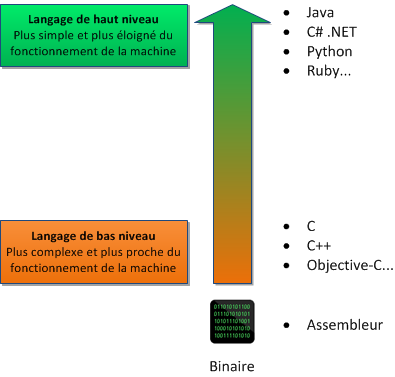
\includegraphics[scale=0.6]{fig/langages.png}
   \caption{(c) OpenClassrooms}
\end{center}
\end{figure}
\end{frame}

\subsection{Historique}

\begin{frame}{Histoire}
\begin{itemize}
\item 1958 : Algol
\item années 60 : CPL, puis BPCL puis B
\item 1970 : langage C (Dennis Ritchie 1969-1973)
\item 1979 : \textit{C with classes}
\item 1983 : C++ (amélioration du C ) : Bjarne Stroustrup
\item 1989 : C++ 2.0 (héritage multiple, classes abstraites)
\item 1995 : java
\item 1998 : début de la normalisation de C++ (inclusion de la \textit{SL})
\item 2011 : \textbf{C++11 devient un standard ISO}
\item 2014 : nouvelle norme C++14
\item 2017 : c++17 : définition figée en avril 2017, acceptation ISO/ANSI
\item 2020 : c++20 : en retard
\end{itemize}
\end{frame}

\begin{frame}[fragile]
   \frametitle{C à l'ancienne}
   \begin{itemize}
      \item Pour mémoire, C est un langage qui permet des choses un peu \emph{roots}
   \end{itemize}
   \pause 
   \begin{lstlisting}
      int a;
      a = a+++++a; // forbidden since C89
   \end{lstlisting}
   \pause
   \begin{lstlisting}
      switch(0)
      i++;
   \end{lstlisting}
   \pause 
   \begin{lstlisting}
      #define boo() 123
      #define foo(y) boo y )
      #define open (
      foo(open)
   \end{lstlisting}
   \pause
   \begin{lstlisting}
      #include<stdio.h>
      int main(){int a=0,b=a;long long c[178819],d=8,e=257,f,g,
      h,i=d-9;for(;a<178819;){c[a++]=i;}for(a*=53;a;a>>=8)putc\
      har(a);if((f=getchar())<0)return 0;for(;(g=getchar())>=0;
      ){h=i=g<<8^f;g+=f<<8;a=e<(512<<a%8|(a<7))||f>256?a:a>6?15
      :a+1;for(;c[i]>-1&&c[i]>>16!=g;)i+=i+h<69000?h+1:h-69000;
      h=c[i]<0;b|=h*f<<d;for(d+=h*(a%8+9);d>15;d-=8)putchar(b=b
      >>8);f=h?g-f*256:c[i]%65536L;if(a<8*h){c[i]=g*65536L|e++;
      }}b|=f<<d;for(d+=a%8;d>-1;d-=8)putchar(b>>=8);return!53;}
   \end{lstlisting}
\end{frame}

\subsection{Organisation du cours}

\begin{frame}{Organisation}
\begin{itemize}
\item Peu de cours, beaucoup de pratique
\item un DS sur table à la fin (évaluation individuelle)
\item Base de travail
\begin{itemize}
\item Norme "C++11-14"
\item Utilisation de la machine virtuelle Linux installée en B114
\item outils : make, gcc
\item IDE ou éditeurs de texte : à votre convenance
\begin{alertblock}{Avertissement}
Vous pouvez utiliser d'autres outils (compilateurs), mais à vos risques et périls !
\end{alertblock}
\end{itemize}
\end{itemize}
\end{frame}

\begin{frame}{A propos des TP}
   \begin{itemize}
      \item Tous les TP rendus sont corrigés 
      \item Aucun TP n'est noté 
      \item En clair
      \begin{itemize}
         \item Chacun travaille à son rythme
         \item Cela ne sert à rien de rendre le TP du voisin parce qu'on est en retard
         \item Lire le C++ $\neq$ écrire le C++ 
         \item On ne peut pas rendre les TP, mais cela consiste à aller au DS sans filet
      \end{itemize}
   \end{itemize}
\end{frame}

\section{Rappels rapides}

% % rappels sur ce qui a été vu en ALGPR
\subsection{Vos (anciens) premiers pas en C++}

\begin{frame}[fragile]
\frametitle{Premier programme C++}
\begin{lstlisting}[language=C++]
#include <iostream>
using namespace std;

/* fonction principale du programme

	Elle affiche un message
*/
int main() {
  cout << "hello world" << endl;

  return 0;
}
\end{lstlisting}
\end{frame}

\begin{frame}{Ligne par ligne}
\begin{itemize}
\item \texttt{\#include <iostream>} : inclure des fichiers de \textbf{déclaration} d'autres fonctions
\item \texttt{using namespace std;}: utiliser un espace de nommage, plus tard !
\item \texttt{/* ... */} définit une zone de commentaires (pas interprétée par le compilateur)
\item \texttt{int main() $\{$ ... $\}$} : fonction principale, appelée au lancement du programme
\item \texttt{cout << "hello world" << endl;} : façon \textit{moderne} d'afficher du texte
\item \texttt{return 0;} : la fonction \textit{main()} est supposée retourner un entier
\end{itemize}
\end{frame}

\begin{frame}[fragile]
\frametitle{Compilation et édition des liens (v1)}
\begin{itemize}
\item Compilation : transformation d'un fichier source en code \textit{objet}
\item Edition des liens : assemblage de plusieurs fichiers objet pour en faire un exécutable (\texttt{.exe} sous Windows, pas d'extension obligatoire sur les autres systèmes)
\end{itemize}
\pause \begin{block}{En ligne de commande}
\begin{verbatim}
g++ -c premierprog.cxx
g++ -o premierprog.out premierprog.o
\end{verbatim}
\end{block}

\pause \begin{exampleblock}{Exécution}
\begin{verbatim}
./premierprog.out
hello world
\end{verbatim}
\end{exampleblock}
\end{frame}

% tous sur les makefiles
\subsection{Makefiles}

\begin{frame}{Motivations}
  \begin{itemize}
  \item Gérer plusieurs fichiers source et l'ensemble du processus de compilation / éditions des liens en une seule opération
  \begin{itemize}
  \item Faire plus ou moins l'équivalent des IDE comme Visual Studio
	\begin{itemize}
		\item Note : il y a moins bien (\texttt{make}), mais il y a aussi beaucoup mieux...
		\item VS ne sait pas gérer le multi-plateformes (et pour cause)
		\item VS ne sait pas trouver vos bibliothèques tout seul
	\end{itemize}
  \item Pour un gros projet : ne recompiler que le strict minimum nécessaire
  \end{itemize}
  \item Rappels : différentes phases
  \begin{itemize}
  \item Compilation des fichiers source (on a encouragé leur multiplication !)
  \item Edition des liens
  \end{itemize}

  \end{itemize}
\end{frame}

\begin{frame}{Principe}
  \begin{itemize}
  \item 2 étapes
  \begin{itemize}
  \item Ecriture d'un fichier \texttt{Makefile} (modifé à chaque fois qu'on ajoute un nouveau fichier source
  \item Compilation/Edition des liens : appel de la commande \texttt{make}
  \end{itemize}
  \begin{exampleblock}{Exemple}
  	Soit un programme exécutable \texttt{machin.out} construit à partir de 3 fichiers source \texttt{main.cxx}, \texttt{f1.cxx} et \texttt{f2.cxx}. Construction :
  	\begin{itemize}
  		\item \texttt{g++ -c main.cxx}
  		\item \texttt{g++ -c f1.cxx}
  		\item \texttt{g++ -c f2.cxx}
  		\item \texttt{g++ -o machin.out main.o f1.o f2.o}
  	\end{itemize}
  \end{exampleblock}
  \end{itemize}
\end{frame}

\begin{frame}{Graphe de dépendances}
  \begin{itemize}
  \item Ecrire quel fichier dépend de quel autre
  \begin{itemize}
  \item \texttt{machin.out} dépend de \texttt{main.o}, \texttt{f1.o} et \texttt{f2.o}
  \item \texttt{main.o} dépend de \texttt{main.cxx}
  \item \texttt{f1.o} dépend de \texttt{f1.cxx}
  \item \texttt{f2.o} dépend de \texttt{f2.cxx}
  \end{itemize}
  \item Les règles permettant de reconstruire les fichiers .out et .o sont connues
  \end{itemize}
      \begin{center}
      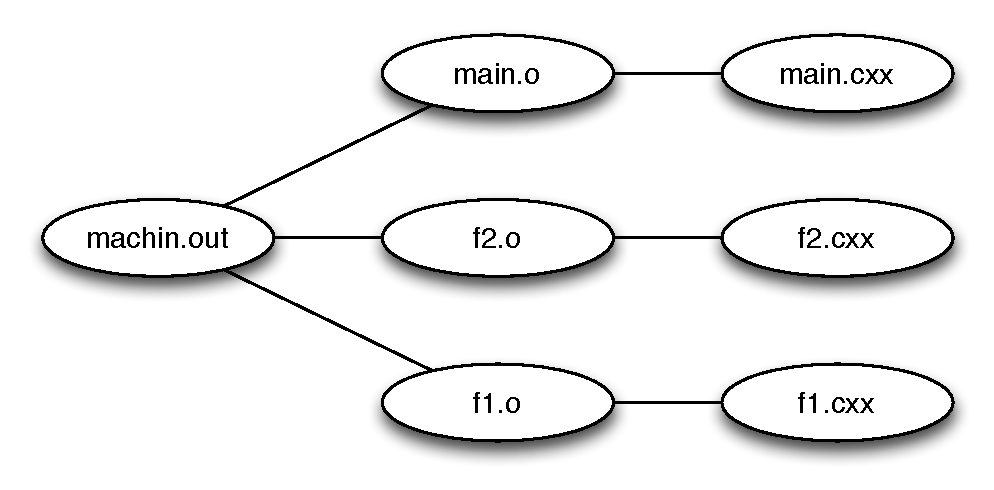
\includegraphics[scale=.43]{fig/base-dependance.pdf}
    \end{center}

\end{frame}

\begin{frame}{Dépendance temporelle}
  \begin{itemize}
  \item La date et l'heure du fichier sont utilisées : un fichier doit toujours être plus récent que les fichiers à sa droite dont il dépend
  \item Si ce n'est pas le cas, l'opération de production du fichier de gauche est lancée
  \item Le processus est itéré jusqu'à ce que toutes les règles soient respectées
  \end{itemize}
\end{frame}

\begin{frame}{Exemple (1/3)}
        \begin{center}
      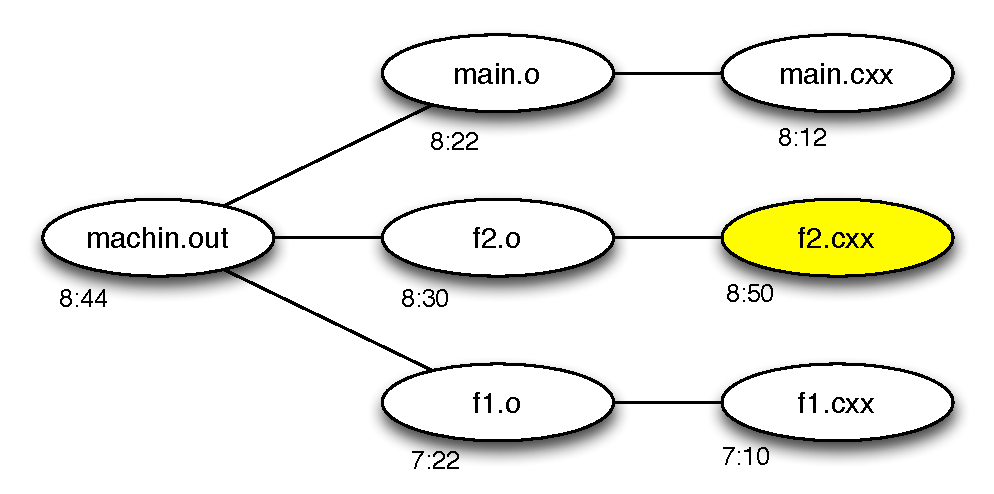
\includegraphics[scale=.6]{fig/base-dependance1.pdf}
    \end{center}
\end{frame}

\begin{frame}{Exemple (2/3)}
        \begin{center}
      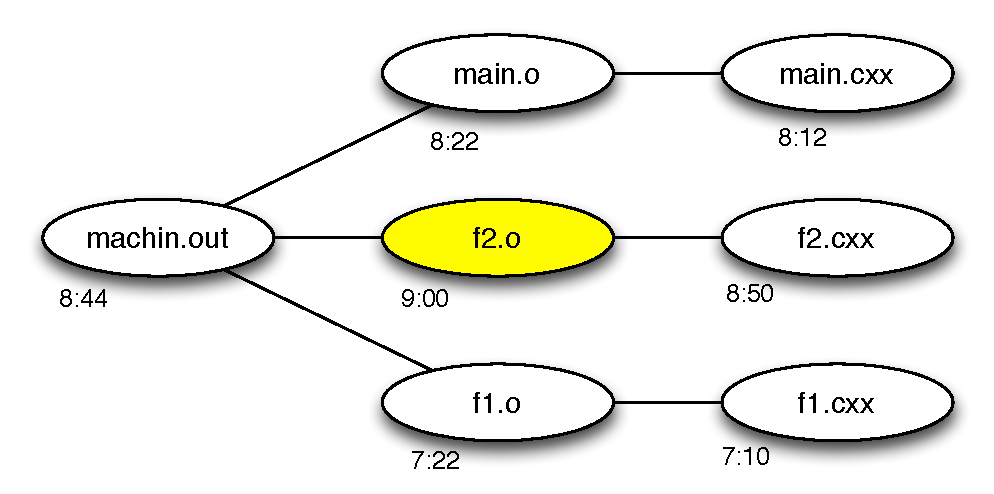
\includegraphics[scale=.6]{fig/base-dependance2.pdf}
    \end{center}
\end{frame}

\begin{frame}{Exemple (3/3)}
        \begin{center}
      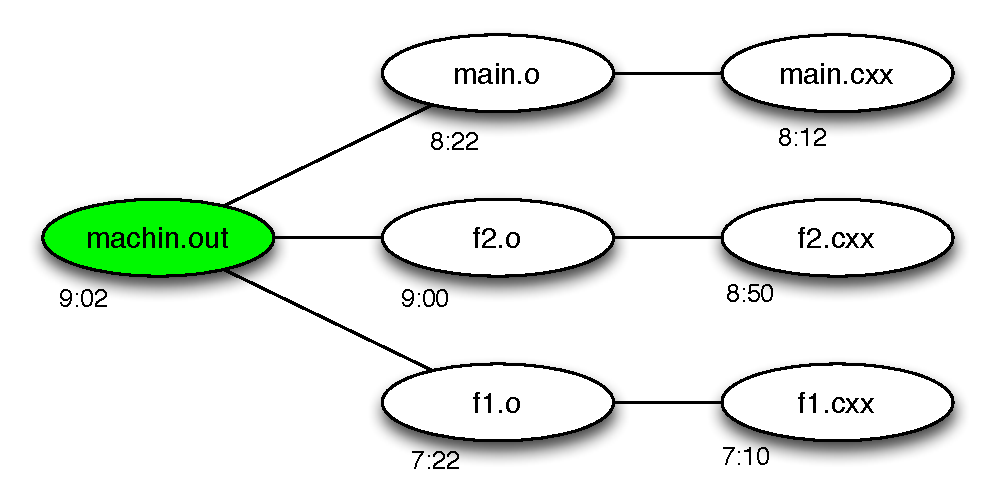
\includegraphics[scale=.6]{fig/base-dependance3.pdf}
    \end{center}
\end{frame}

\begin{frame}{Syntaxe du \texttt{Makefile}}
\begin{block}{Ensemble de règles de la forme}
\texttt{  fichier: fichier1 fichier2 fichier3 ... \\
  	<TAB>régle de production de fichier \\
}\end{block}
\begin{itemize}
\item Note : le fichier s'appelle obligatoirement \texttt{Makefile}
\begin{itemize}
\item Sauf parfois sous Windows, qui n'aime pas les fichiers sans extensions...
\end{itemize}
\item La première règle est toujours celle qui produit l'exécutable
\begin{itemize}
	\item en fait non, c'est juste celle qui sera vérifiée en premier par \texttt{make}
\end{itemize}
\item Ensuite il suffit d'appeler la commande \texttt{make}
\end{itemize}
\end{frame}

\begin{frame}[fragile]
  \frametitle{Makefile de l'exemple}
        \begin{center}
      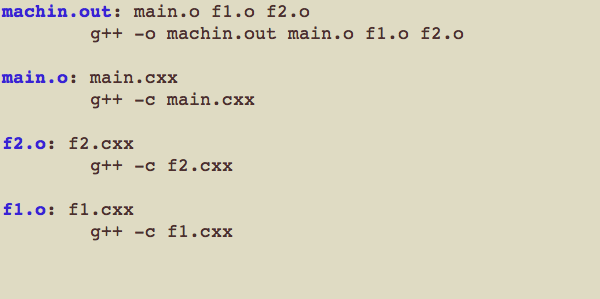
\includegraphics[scale=.4]{fig/makefile.png}
    \end{center}
\end{frame}


\subsection{Syntaxe générale du langage C(++)}

\begin{frame}[fragile]
\frametitle{Commentaires}
\begin{lstlisting}[language=C++]
/* Ceci est un commentaire qui peut etre long */

// Ceci est un commentaire d'une ligne
\end{lstlisting}
\begin{itemize}
\item nécessaires (mais pas suffisants) à se remettre dans le code 6 mois plus tard
\item nécessaires (mais pas suffisants) pour donner son code à quelqu'un d'autre
\item Éléments de qualité du code (métriques)
\end{itemize}

\end{frame}


\begin{frame}[fragile]
\frametitle{Types de base en C(++)}
\begin{itemize}
\item Entiers
\begin{itemize}
\item caractères : \verb|char| (entiers sur 8 (?) bits)
\item entiers classiques : \verb|int|, \verb|short| (16 bits), \verb|long| (32 bits), \verb|long long| (64 bits)
\item utilisation possible des préfixes \verb|signed| et \verb|unsigned|
\item il existe aussi des types de taille fixe : \verb|int8_t|, \verb|uint8_t|,... définis dans \verb|stdint.h|
\end{itemize}
\item types flottants
\begin{itemize}
\item simple précision : \verb|float|
\item double précision : \verb|double|
\end{itemize}
\item Les constantes sont préfixées par \verb|const|
\end{itemize}
\end{frame}

\begin{frame}[fragile]
\frametitle{Enregistrements}
\begin{itemize}
\item Définition d'un enregistrement
\begin{lstlisting}
struct nomtype {
	type1 attribut1;
	...
	typeN attributN;
};
\end{lstlisting}
\begin{codeblock}{Exemple}
\begin{lstlisting}
struct complexe {
	float re,im;
};
\end{lstlisting}
\end{codeblock}
\item Déclaration d'une variable de type enregistrement : \verb|nomtype nomvar;|
\item Accès aux attributs : \verb|nomvar.attributI|
\item La comparaison directe \verb|==| n'est pas possible, mais la copie (superficielle) est possible avec \verb|=|
\end{itemize}
\end{frame}

\begin{frame}[fragile]
\frametitle{Blocs d'instructions}
\begin{itemize}
\item instruction simple \verb|<I> : I;|
\item Bloc d'instructions \verb|<B> : { I1; ... IN; }|
\item En C, les déclarations de variables doivent se faire en \textbf{début de bloc}. En C++, on peut les faire n'importe où, mais ce n'est pas recommandé pour autant
\item Portée des variables : bloc d'instructions dans lequel elles sont déclarées
\end{itemize}
\end{frame}

\begin{frame}[fragile]
\frametitle{Opérateurs}
\begin{itemize}
\item Affectation : \verb|=|
\item Arithmétique :
\begin{itemize}
\item addition : \verb|+|
\item soustraction : \verb|-|
\item multiplication : \verb|*|
\item division : \verb|/|
\item modulo : \verb| %|
\end{itemize}
\item Opérateurs raccourcis : \verb|+=,-=,*=,/=|...
\item Incrémentation, décrémentation : \verb|++| et \verb|--| sous forme préfixe ou suffixe
\item Opérations sur les bits :
\begin{itemize}
\item \verb#&,|,^# : et, ou, ou exclusif
\item décalages bit à bit : \verb|<<| et \verb|>>|
\end{itemize}
\item Opérateur ternaire \verb|(| \textit{condition} \verb|?| \textit{action1} \verb|:| \textit{action2} \verb|)|
\end{itemize}
\end{frame}

\begin{frame}[fragile]
\frametitle{Structures de contrôle}
\begin{itemize}
\item Syntaxe 1 : \verb|if (|\textit{condition}\verb|)| \textit{bloc1}
\item Syntaxe 2 : \verb|if (|\textit{condition}\verb|)| \textit{bloc1} \verb|else| \textit{bloc2}
\item \alert{Attention} : les parenthèses autour de la condition sont obligatoires
\item \textit{condition} est une expression de type booléen (\verb|int| en C à l'ancienne qui n'a pas de type de booléen)
\begin{itemize}
\item 0 pour faux, n'importe quelle autre valeur est vraie
\end{itemize}
\item Opérateurs pour les expressions booléennes
\begin{itemize}
\item \verb|&&|, \verb#||#, \verb|!|, \verb|==|, \verb|!=|
\item ainsi évidemment que \verb|<|, \verb|<=|, \verb|>=|, \verb|>|
\end{itemize}
\item Opérateur de sélection : \verb|switch(|\textit{var-num}\verb|) {| \textit{liste de cas} \verb|}|
\begin{itemize}
\item cas : \verb|case |\textit{nombre}\verb|:| \textit{liste d'instructions} \verb|break;|
\item cas par défaut (en dernier) : \verb|default:|  \textit{liste d'instructions}
\end{itemize}
\end{itemize}
\end{frame}

\begin{frame}[fragile]
\frametitle{Structures itératives}
\begin{itemize}
\item \verb|while (|\textit{condition}\verb|) {| \textit{liste d'instructions} \verb|}| : répète la liste d'instructions tant que la condition \textit{condition} est vraie
\begin{itemize}
\item La condition est évaluée \structure{avant} chaque exécution de la liste d'instructions
\end{itemize}
\item \verb|for (|\textit{initialisation} \verb|;| \textit{invariant} \verb|;| \textit{incrément} \verb|) {| \textit{liste d'instructions} \verb|}|
\begin{itemize}
\item La liste d'instructions est exécutée tant que l'invariant est vrai (vérifié avant chaque entrée dans la boucle
\item L'incrément est effectué juste avant de vérifier la condition
\end{itemize}
\item \verb|do {| \textit{liste d'instructions} \verb|} while (| \textit{condition} \verb|);|  : répète la liste d'instructions tant que la condition \textit{condition} est vraie
\begin{itemize}
\item La condition est évaluée \structure{après} chaque exécution de la liste d'instructions
\end{itemize}
\item \verb|break| sort de la structure de répétition correspondante
\item \verb|continue| passe immédiatement à l'itération suivante
\end{itemize}
\end{frame}

\begin{frame}[fragile]
\frametitle{Fonctions}
\begin{itemize}
\item Définition d'une fonction : \textit{typeretour} \verb|nom_fonction(| \textit{liste de paramètres} \verb|) {|  \textit{liste d'instructions }\verb|}|
\begin{itemize}
\item liste de paramètres : \textit{type1} \textit{nom1}, ..., \textit{typeN} \textit{nomN}
\item retour de la fonction : \verb|return| \textit{val}\verb|;|
\item \textit{val} doit être de type \textit{typeretour} ou omis si \textit{typeretour} \verb|void|
\item \textit{typeretour} possibles : types simples, structures, pointeurs, \verb|void|
\item Les paramètres sont des variables locales des fonctions (copie des valeurs passées à l'appel)
\end{itemize}
\item Déclaration (prototype, signature)
\begin{itemize}
\item \textit{typeretour} \verb|nom_fonction(| \textit{liste de paramètres} \verb|);|
\end{itemize}
\end{itemize}
\end{frame}

\subsection{La gestion de la mémoire en C}

%% tout sur les pointeurs

\subsubsection{Pointeurs}

\begin{frame}{Retour sur les pointeurs}
\begin{center}
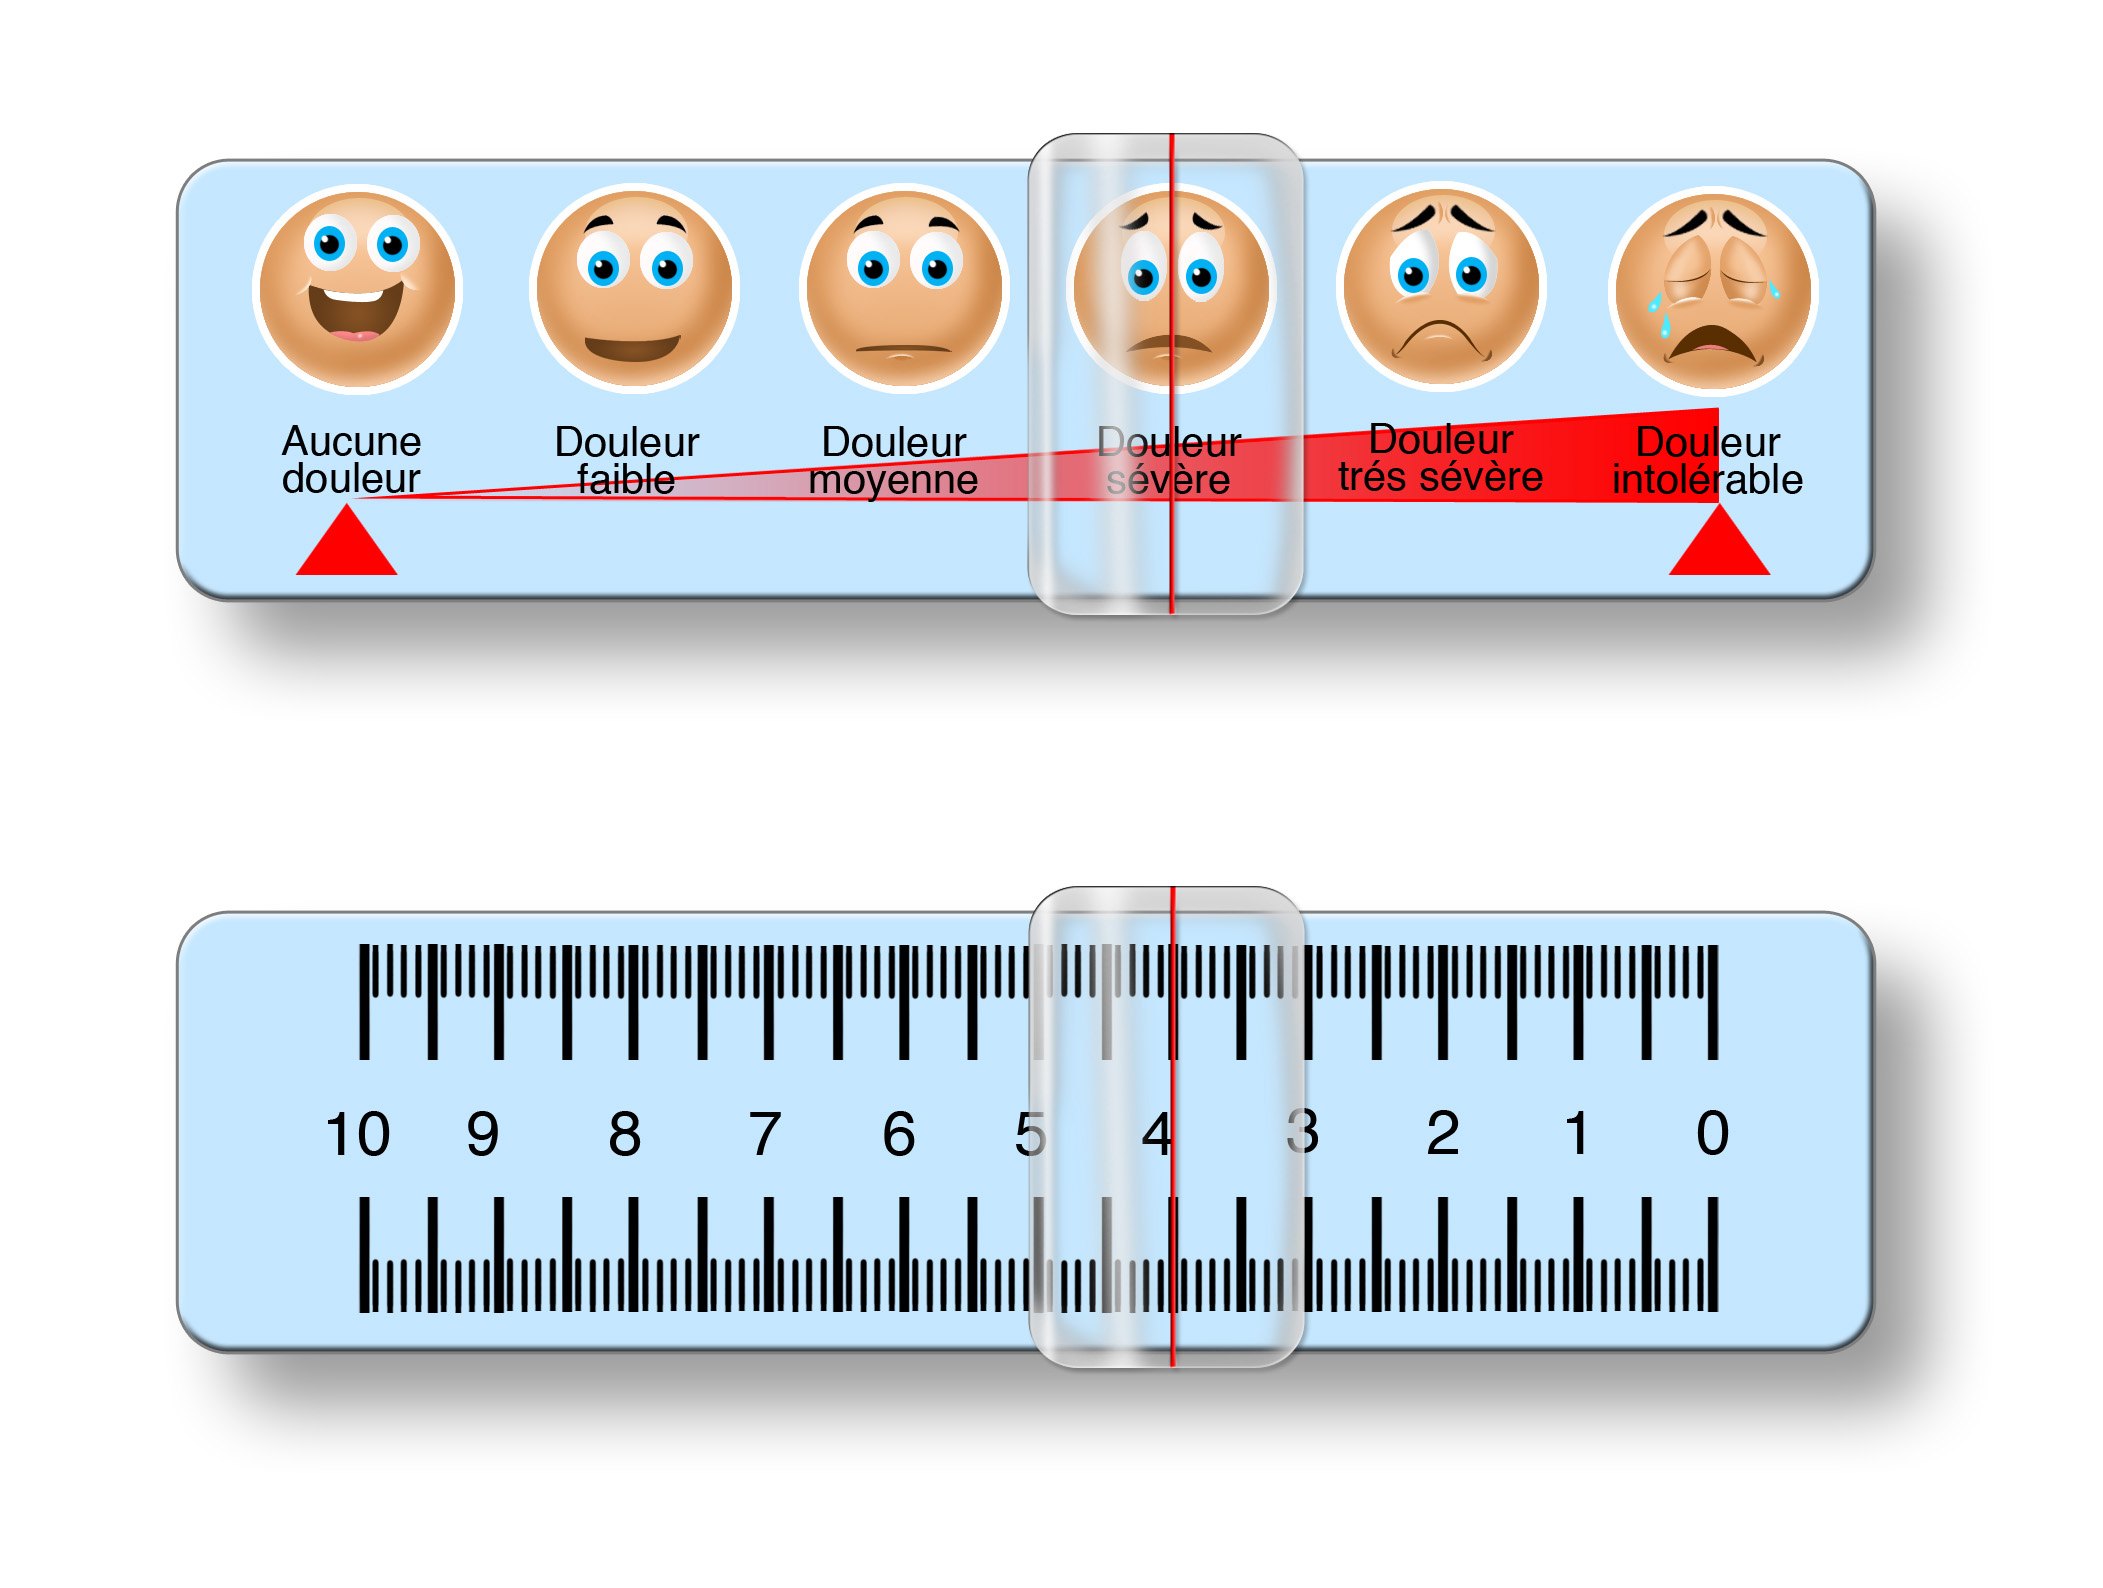
\includegraphics[height=.8\textheight]{fig/echelle-douleur.jpg}
\end{center}
\end{frame}

\begin{frame}{Organisation de la mémoire d'un ordinateur}
\begin{itemize}
\item Elle peut être vue comme un tableau d'octets avec :
\begin{itemize}
\item en \textit{indice} : le numéro de la case mémoire (commençant à 0) appelée l'\textbf{adresse}
\item en \textit{valeur} : la valeur de l'octet de la case mémoire référencée par l'indice
\end{itemize}
\end{itemize}
\begin{center}
\begin{tabular}{|l|l|}
\hline \textbf{adresse} & \textbf{valeur} \\
\hline 0 & ? \\
1 & ? \\
... & \\
234532 & 244 \\
... & \\
$n-1$ & \\
\hline
\end{tabular}
\end{center}
\end{frame}

\begin{frame}[fragile]
\frametitle{Déclaration d'une variable locale}
\begin{itemize}
\item Que se passe-t-il lorsqu'on déclare une variable ?
\begin{lstlisting}
char x = 'a';
\end{lstlisting}
\item Le système réserve une place en mémoire qui contient la valeur de \texttt{x}
\begin{itemize}
\item Il trouve une place libre (par exemple 22222)
\item dans la case associée, il stocke la valeur de la variable (ici \texttt{'a'})
\end{itemize}
\end{itemize}
\begin{center}
\begin{tabular}{|l|l|}
\hline \textbf{adresse} & \textbf{valeur} \\
\hline 0 & ? \\
1 & ? \\
... & \\
22222 & \texttt{'a'} \\
... & \\
$n-1$ & \\
\hline
\end{tabular}
\end{center}
\end{frame}

\begin{frame}[fragile]
\frametitle{Adresse d'une variable}
\begin{itemize}
\item En C(++), on peut demander l'adresse d'une variable : il suffit de préfixer son nom avec \&
%\begin{lstlisting}
%&x
%\end{lstlisting}
\item \texttt{\&x} représente l'adresse de \texttt{x}, c'est-à-dire 22222
\item Les adresses sont de simples entiers, mais C(++) permet de les typer par sécurité
\item Pointeur sur le type \textit{t} = adresse d'une variable de type \textit{t}
\item Exemples
\begin{itemize}
\item pointeur sur un entier : \texttt{int *}
\item pointeur sur un caractère : \texttt{char *}
\end{itemize}
\end{itemize}
\begin{lstlisting}
char *ptrX;
ptrX = &x;
\end{lstlisting}
\end{frame}

\begin{frame}[fragile]
\frametitle{Déréférencement}
\begin{itemize}
\item Déréférencement : accéder à la case mémoire \textit{pointée} par une adresse \texttt{t}
\item notation : \texttt{*t}
\end{itemize}
\begin{lstlisting}
cout << x << endl;
cout << *ptrX << endl;
\end{lstlisting}
\pause\begin{exampleblock}{Jouons un peu : qu'affiche ce bout de code ?}
\begin{lstlisting}
int a = 123;
int *x = &a;
*x = 342;
cout << a << endl;
cout << *x << endl;
\end{lstlisting}
\end{exampleblock}
\pause\begin{block}{Réponse}
342 \\
342
\end{block}
\end{frame}


% application des pointeurs

\begin{frame}[fragile]
\frametitle{Application des pointeurs : modifications des paramètres d'une fonction}
\begin{itemize}
\item Exemple d'une fonction qu'on ne sait pas écrire sans pointeurs : échange de deux variables
\item Passage par adresse (par opposition au passage par valeur)
\end{itemize}
\begin{lstlisting}
void echange(int *a,int *b) {
  int c = *a;
  *a = *b;
  *b = c;
}

// appel
int x = 124;
int y = 653;
echange(&x,&y);
cout << x << "," << y << endl;
\end{lstlisting}

\end{frame}

\begin{frame}[fragile]
\frametitle{Application des pointeurs : fonction retournant plusieurs valeurs}
\begin{lstlisting}
void sommediff(int a,int b,int *somme,int *diff) {
  *somme = a+b;
  *diff = a-b;
}

// appel
int s,d;
sommediff(23,18,&s,&d);
cout << s << "," << d << endl;
\end{lstlisting}

\end{frame}

% passage par adresse
\begin{frame}{Passage par adresse}
\begin{itemize}
\item Passer un paramètre à une fonction consiste à ce que la fonction reçoive \textbf{une copie} du paramètre dans une variable (qui porte le même nom ou pas)
\item Conséquence : si on modifie la copie, l'original n'est pas affecté
\item Que se passe-t-il si le paramètre est un pointeur ?
\begin{itemize}
\item Une \textbf{copie du pointeur} est fournie à la fonction appelée
\item La valeur de la copie (l'adresse) pointée ne sera jamais modifiée
\item Mais le contenu peut l'être par déréférencement
\end{itemize}
\end{itemize}
\end{frame}

\begin{frame}[fragile]
\frametitle{Rappel : pointeurs et structures de données}
\begin{itemize}
\item Si on a un type $A$ défini par \texttt{struct} ou \texttt{class}, un pointeur se définit par \texttt{A* ptr}
\item Comment accéder à un attribut \texttt{attr} de $A$ associé à \texttt{ptr} ?
\begin{itemize}
\item Logiquement : \texttt{(*ptr).attr} (attention aux priorités)
\item Raccourci : C(++) fournit une notation plus simple : \texttt{ptr->attr}
\end{itemize}
\item Attention : si le pointeur n'est pas initialisé, le déréférencement est une activité risquée...
\end{itemize}
\begin{exampleblock}{Exemple}
\begin{lstlisting}[language=C++]
int x;
int *y;
int z=*y;
\end{lstlisting}
\end{exampleblock}
\end{frame}

\subsubsection{Allocation dynamique de mémoire}

\begin{frame}[fragile]
\frametitle{Allocation mémoire en C}
\begin{itemize}
\item Allocation dynamique : réserver de la mémoire pendant l'exécution du programme
\item Réservation de mémoire avec \texttt{malloc}
\begin{lstlisting}
#include <stdio.h>
...
int *a = malloc(sizeof(int)));
struct machin *b = malloc(sizeof(struct machin));
// tableau
int *c = malloc(10*sizeof(int));
c[0] = 1; c[1] = 3;
\end{lstlisting}
\item l'opérateur \texttt{sizeof()} permet de connaître la taille d'une structure de données
\item Libération avec \texttt{free}
\begin{lstlisting}
free(a);
free(b);
free(c);
\end{lstlisting}
\end{itemize}
\end{frame}

\begin{frame}{Remarques}
\begin{itemize}
\item Penser à bien utiliser \texttt{sizeof()}, la taille des structures dépend de l'environnement d'exécution
\item De fait \texttt{malloc} et \texttt{free} ne sont pas typés et fonctionnent avec des \texttt{void *}
\item Ce sont de simples fonctions standard, on peut en utiliser d'autres (API Win32 par exemple)
\item Paradigme de gestion explicite de la mémoire : libérer tout ce qu'on alloue, par opposition au système de \textit{garbage collecting} à la Java
\item Mémoire pas initialisée + opérateurs pas typés + gestion explicite de la mémoire + accès tableaux pas vérifiés = une proportion significative de plantage des programmes C
\end{itemize}
\end{frame}

\begin{frame}[fragile]
\frametitle{Allocation mémoire en C++}
\begin{itemize}
\item Cela ne va pas résoudre tous les problèmes !
\item Réservation de mémoire avec l'opérateur \texttt{new}
\begin{lstlisting}
int *a = new int;
machin *b = new machin;
int *c = new int[10];
\end{lstlisting}
\item Plus besoin de spécifier la taille, plus de problème de type
\item Libération de la mémoire
\begin{lstlisting}
delete a;
delete b;
delete[] c;
\end{lstlisting}
\item Attention, il y a un piège !
\end{itemize}
\end{frame}

\begin{frame}[fragile]
\frametitle{Tableaux et pointeurs}
\begin{itemize}
\item Notion d'arithmétique de pointeurs...
\begin{lstlisting}
void f1() {
    int *a = new int[10];
    int *b = a;
    int i=0;
    while (i<9) {
        *b = i;
        b++; i++;
    }
    *b = i;

    for (int j=0 ; j<10 ; j++) {
        cout << "a[" << j << "] = " << a[j] << endl;
    }

    delete[] a;
}
\end{lstlisting}
\item On peut appliquer additions et soustractions aux pointeurs
\begin{itemize}
\item l'unité est la taille du type de l'élément pointé
\item utile pour parcourir vite des tableaux, mais dangereux à souhait
\item aucune vérification de validité n'est effectuée...
\end{itemize}
\end{itemize}
\end{frame}
% arithmetique de pointeurs

% effets de bord
\begin{frame}{Exercice}
\begin{itemize}
\item Écrire un petit bout de code qui parcourt un tableau avec des pointeurs en dépassant la taille du tableau
\item Que se passe-t-il
\begin{itemize}
\item s'il n'y a rien d'autre dans la fonction ?
\item si juste après la déclaration du tableau, d'autres variables sont déclarées ?
\end{itemize}
\item La réponse dépend du compilateur...
\end{itemize}
\end{frame}
% le pointeur void * et les conversions de type

\begin{frame}[fragile]
\frametitle{Le pointeur void *}
\begin{itemize}
\item On a vu que certaines fonctions retournaient un type \texttt{void *}
\item \textit{void} en anglais signifie "rien, nul", voir fonction qui ne retourne rien
\item Que signifie alors \texttt{void *} ? juste une adresse en mémoire, non typée
\item Attention : c'est un format d'échange de tout vers n'importe quoi...
\begin{lstlisting}
    int a[10];
    float *b;

    b = (float *)((void *) a);
\end{lstlisting}
\end{itemize}
\end{frame}
% lien entre pointeurs et tableaux

% un bout sur les smart pointers ?



\section{Classes et objets}

% % C++ et les objets

\subsection{Programmation objet}

\subsection{Les objets}
\subsubsection*{Généralités}

%%%%%%%%%%%%%%%%%%%%%%%%%%%%%%%%%%%%%%%%%%%%%
\begin{frame}{Qu'est-ce qu'un objet ?}
\begin{itemize}
	\item \textbf{modélise} toute entité identifiable, concrète ou abstraite, manipulée par une application logicielle
	\begin{itemize}
		\item une chose tangible : une ville, un étudiant, un bouton sur l'écran
		\item une chose conceptuelle : une date, une réunion, un planning de réservation
	\end{itemize}
	\item \textbf{réagit} à certains messages qu'on lui envoie de l'extérieur ; la réaction détermine le \textbf{comportement} de l'objet
	\item ne réagit pas toujours de la même façon à un même message ; sa réaction dépend de l'\textbf{état dans lequel il se trouve}
\end{itemize}
\end{frame}

%%%%%%%%%%%%%%%%%%%%%%%%%%%%%%%%%%%%%%%%%%%%%
\begin{frame}{Un objet possède : }
\begin{itemize}
	\item une \textbf{identité unique} (pour distinguer un objet d'un autre)
	\item un \textbf{état interne} donné par la valeur d'un certain nombre de variables
	qu'on appelle des \textbf{attributs}
	\begin{itemize}
		\item les attributs décrivent l'état de l'objet à un instant donné (cet homme mesure 1,75m, pèse 54 kg et s'appelle Charles)
		\item les attributs sont typés et nommés (attribut \textit{taille} de type réel)
	\end{itemize}
	\item un \textbf{comportement} (capacités d'action de l'objet) donné par des fonctions qu'on appelle des méthodes (ou opérations)
	\begin{itemize}
		\item les méthodes définissent ce que l'objet peut faire et comment il peut le faire
 	\end{itemize}
\end{itemize}
\end{frame}

%%%%%%%%%%%%%%%%%%%%%%%%%%%%%%%%%%%%%%%%%%%%%
\begin{frame}{Objet = données + algorithmes}
\begin{itemize}
	\item un objet est le regroupement de données (attributs) et des traitements associés (méthodes)
	\item Principe d'\textbf{encapsulation} : séparer les données des traitements
\end{itemize}
  \begin{figure}[htbp]
    \begin{center}
      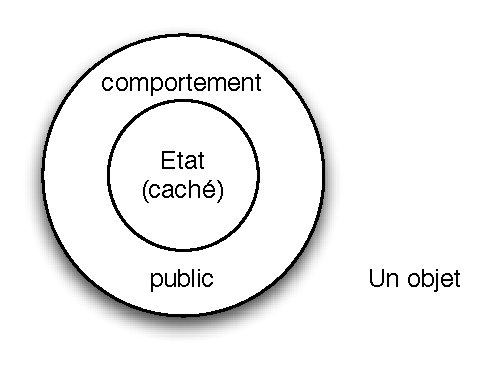
\includegraphics[scale=.5]{fig/encapsulation.pdf}
    \end{center}
  \end{figure}
\end{frame}

\subsubsection*{Encapsulation}

%%%%%%%%%%%%%%%%%%%%%%%%%%%%%%%%%%%%%%%%%%%%%
\begin{frame}{Principe d'encapsulation}
\begin{itemize}
	\item L'accès aux données (état) de l'objet ne peut être fait qu'au travers des méthodes
	\begin{itemize}
		\item les données sont \textbf{privées} (cachées)
		\item les méthodes \textbf{publiques} définissent l'\textbf{interface} de l'objet
	\end{itemize}
	\item Intérêt : la modification des structures de données n'affecte pas les programmes qui utiliseront l'objet
	\begin{itemize}
		\item masquage de l'implémentation : robustesse du code
		\item facilité d'évolution du logiciel
		\item pas de modification de l'interface
	\end{itemize}
\end{itemize}
\end{frame}

\subsubsection{Exemple}

% pour mémoire, ils ont déjà vu les string

\begin{frame}[fragile]
\frametitle{Déjà vus : les objets \texttt{string}}
\begin{itemize}
\item Pas de vrai type chaîne de caractère en C
\item ALGPR : Utilisation du type \texttt{string} de C++
\item En réalité le type \texttt{string} est beaucoup plus puissant que l'utilisation faite l'an dernier
\end{itemize}
\begin{exampleblock}{Utilisation}
\begin{lstlisting}
string maChaine("toto");

cout << maChaine << endl;

string maChaine2 = "titi";

cout << maChaine2 << endl;

string maChaine3 = maChaine+maChaine2;

cout << maChaine3 << endl;
\end{lstlisting}
\end{exampleblock}
\end{frame}
%%%%%%%%%%%%%%%%%%%%%%%%%%%%%%%%%%%%%%%%%%%%%
\begin{frame}{{\href{code/Pendule.cxx}{\scalebox{.25}{
\includegraphics{fig/codeicon}}}} Exemple : un objet pendule}
  \begin{figure}[htbp]
    \begin{center}
      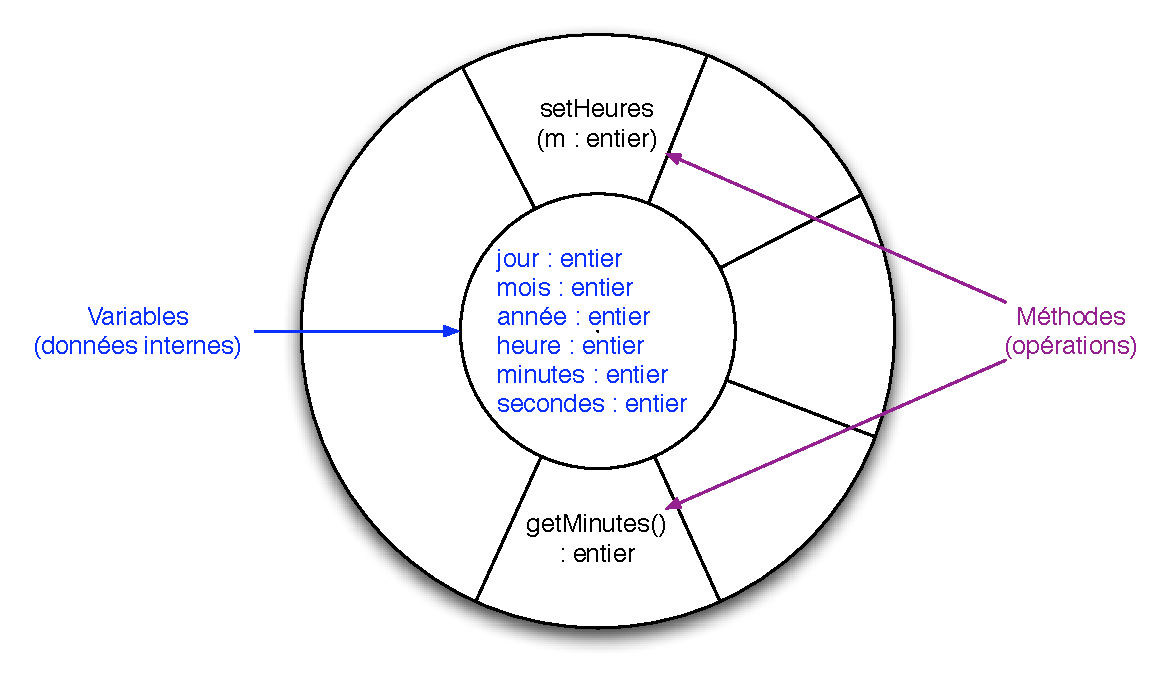
\includegraphics[scale=.45]{fig/encapsulation2.pdf}
    \end{center}
  \end{figure}
\end{frame}

\begin{frame}[fragile]
\frametitle{classe Pendule (1/2)}
\lstinputlisting[linerange=1-29]{code/pendule.cxx}
\end{frame}

\begin{frame}[fragile]
\frametitle{classe Pendule (2/2)}
\lstinputlisting[linerange=30-61]{code/pendule.cxx}
\end{frame}

\subsubsection*{Communication par messages}

%%%%%%%%%%%%%%%%%%%%%%%%%%%%%%%%%%%%%%%%%%%%%
\begin{frame}{Communication par messages}
\begin{block}{Communication}
Les objets \textbf{interagissent} et \textbf{communiquent} entre eux par l'envoi de \textbf{messages}
\end{block}
\begin{itemize}
\pause	\item Les méthodes publiques d'un objet correspondent aux messages que l'on peut lui envoyer
\pause	\item Les messages sont caractérisés par :
	\begin{itemize}
		\pause \item l'objet cible (récepteur) du message
		\pause \item le nom de la méthode à déclencher
		\pause \item les paramètres de cette méthode
	\end{itemize}
\end{itemize}
\end{frame}

%%%%%%%%%%%%%%%%%%%%%%%%%%%%%%%%%%%%%%%%%%%%%
\begin{frame}{\'Echange de messages}
\begin{center}
	Les objets s'envoient des messages entre eux
\end{center}
  \begin{figure}[htbp]
    \begin{center}
      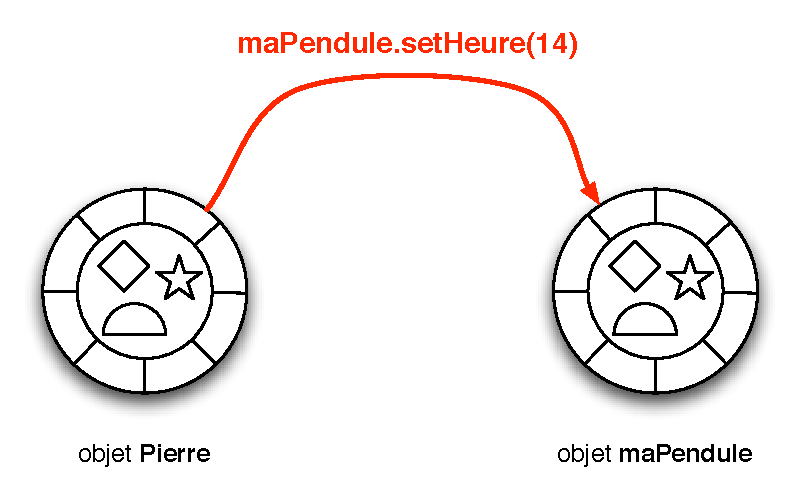
\includegraphics[scale=.55]{fig/messages.pdf}
    \end{center}
  \end{figure}
\end{frame}

\subsubsection*{Classes et instances}

%%%%%%%%%%%%%%%%%%%%%%%%%%%%%%%%%%%%%%%%%%%%%
\begin{frame}{Classes et instances}
\begin{itemize}
	\item Les objets (instances) sont créés (instanciés) à partir de <<moules>> qu'on appelle des \textbf{classes}
	\item classe = schéma, moule, modèle d'objets décrivant :
	\begin{itemize}
	\item partie privée : structure de données interne (attributs), corps des méthodes (algorithmes)
	\item partie publique (interface) : noms et paramètres des méthodes
	\end{itemize}
	\item la classe est un générateur d'objet : par \textbf{instanciation}, on peut fabriquer des objets (instances) respectant ce schéma/moule/modèle
\end{itemize}
\end{frame}

\begin{frame}{Vue duale}
\begin{itemize}
	\item Une \textbf{classe} est un \textbf{modèle} de définition pour des objets
	\begin{itemize}
		\item ayant même structure (même ensemble d'attributs)
		\item ayant même comportement (mêmes opérations, méthodes)
		\item ayant une sémantique commune
	\end{itemize}
	\item Les \textbf{objets} sont des représentations \textbf{dynamiques} (instanciation)
	<<vivantes>> du modèle défini pour eux au travers de la classe
	\begin{itemize}
		\item Une classe permet d'\textbf{instancier} (créer) plusieurs objets
		\item Chaque objet est \textbf{instance} d'une (seule) classe
	\end{itemize}
\end{itemize}
\end{frame}


%%%%%%%%%%%%%%%%%%%%%%%%%%%%%%%%%%%%%%%%%%%%%
\begin{frame}{Classes et instances}
\begin{center}
	La classe Pendule est le moule commun des deux objets
\end{center}
  \begin{figure}[htbp]
    \begin{center}
      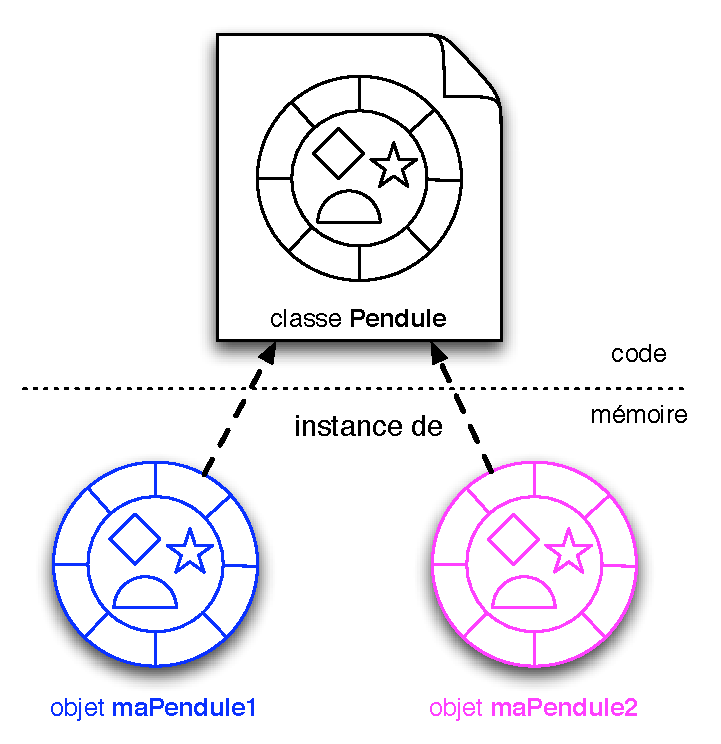
\includegraphics[scale=.37]{fig/instances.pdf}
    \end{center}
  \end{figure}
\end{frame}

\subsubsection*{Hiérarchie de classes}

%%%%%%%%%%%%%%%%%%%%%%%%%%%%%%%%%%%%%%%%%%%%%
\begin{frame}{Hiérarchie de classes}
\begin{itemize}
	\item les classes peuvent être des raffinements/spécialisations de classes existantes
	\item Elles forment alors une \textbf{hiérarchie de classes} où chaque classe :
	\begin{itemize}
		\item \textbf{hérite} des attributs et des méthodes de ses ancêtres (super-classe)
		\item ajoute de nouveaux attributs et/ou de nouvelles méthodes
		\item peut modifier ou redéfinir les méthodes héritées
	\end{itemize}
	\item Intérêt de l'héritage :
	\begin{itemize}
		\item réutilisation du code
		\item pas besoin de réinventer la roue à chaque fois
	\end{itemize}
\end{itemize}
\end{frame}

\begin{frame}{Hiérarchie de classes : exemple}
  \begin{figure}[htbp]
    \begin{center}
      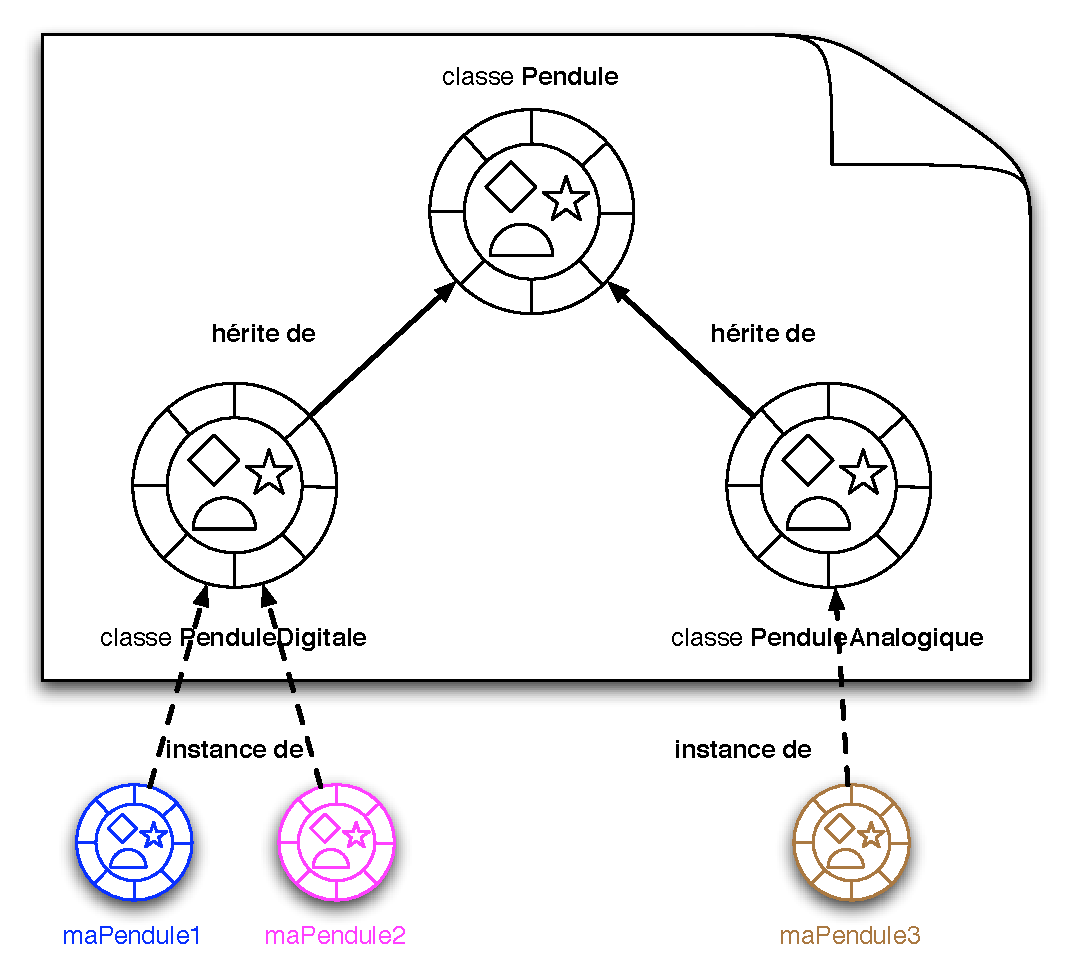
\includegraphics[scale=.32]{fig/heritage.pdf}
    \end{center}
  \end{figure}
\end{frame}

\subsection{Approche orientée-objet}

%%%%%%%%%%%%%%%%%%%%%%%%%%%%%%%%%%%%%%%%%%%%%
\begin{frame}{Approche orientée-objet}
\begin{itemize}
	\pause \item Rappel : approche procédurale
	\begin{itemize}
		\item Définir les structures de données
		\item Définir les traitements (analyse descendante)
		\item Le programme principal enchaîne les traitements
	\end{itemize}
	\pause \item Approche orientée-objet
	\begin{itemize}
		\item modéliser le monde de l'application avec des objets
	\end{itemize}
\end{itemize}
\end{frame}

\begin{frame}{Approche orientée-objet}
	\begin{itemize}
		\pause \item Identifier les classes
		\pause \item Pour chaque classe
		\begin{itemize}
			\item Définir son interface publique (quoi)
			\item Définir son implémentation (comment)
		\end{itemize}
		\pause \item Le programme principal
		\begin{itemize}
			\item création (instanciation) d'objets en mémoire
			\item lance l'exécution par envoi de messages aux objets créés
			\item ces messages peuvent provoquer d'autres envois de messages et/ou
			la création d'autres objets
		\end{itemize}
	\end{itemize}
\end{frame}

\subsection{Les classes en C++}

\begin{frame}{Déclaration de classe en C++}
\begin{definition}
\texttt{class} \textit{nom} \{ \\
...
\} ;
\end{definition}

\begin{itemize}
\item Attention : le point-virgule à la fin est obligatoire !
\item A l'intérieur de la classe :
\begin{itemize}
\item Attributs
\item Méthodes (ou déclaration de méthodes)
\item Indicateurs de protection
\end{itemize}
\end{itemize}
\end{frame}

\begin{frame}[fragile]
\frametitle{Déclaration des attributs}
\begin{definition}
\textit{type} \textit{nom}  ;
\end{definition}
\begin{itemize}
\item Le \textit{type} peut être un type de base ou un type objet
\item Si c'est un type objet, création d'une nouvelle instance
\end{itemize}
\begin{exampleblock}{Exemple}
\begin{lstlisting}
int jour;
Pendule maPendule;
string maChaine;
int *pJour;
\end{lstlisting}
\end{exampleblock}
\end{frame}

\begin{frame}[fragile]
\frametitle{Déclaration des méthodes}
\begin{itemize}
\item Déclaration et définition simultanées
\begin{definition}
\textit{typederetour} \textit{nom} ( \textit{listedeparamètrestypés} ) \{ \\
\texttt{// corps de la méthode} \\
\}
\end{definition}
\item Déclaration seule (classe dans un fichier .h)
\begin{definition}
\textit{typederetour} \textit{nom} ( \textit{listedeparamètrestypés} ) ;
\end{definition}
\item Définition (dans le fichier .cxx)
\begin{definition}
\textit{typederetour} \texttt{\textit{nomdeclasse}::\textit{nom}} ( \textit{listedeparamètrestypés} ) \{ \\
\texttt{// corps de la méthode} \\
\}
\end{definition}
\end{itemize}
\end{frame}

\begin{frame}[fragile]
\frametitle{classe exemplemeth1 : un seul fichier}
\lstinputlisting{code/exemplemeth1.cxx}
\end{frame}

\begin{frame}[fragile]
\frametitle{classe exemplemeth2 : deux fichiers}
\lstinputlisting{code/exemplemeth2.h}
\end{frame}

\begin{frame}[fragile]
\frametitle{classe exemplemeth2 : deux fichiers}
\lstinputlisting{code/exemplemeth2.cxx}
\end{frame}

\begin{frame}[fragile]
\frametitle{Exécution}
\begin{block}{Résultat d'exécution}
{\tiny \begin{verbatim}
[MacBook-Pro-de-Guillaume-2:optionRV/CPLUS/code] moreau% Debug/exemplemeth1
2
3
a = 2
b = 3
5
[MacBook-Pro-de-Guillaume-2:optionRV/CPLUS/code] moreau% Debug/exemplemeth2
2
3
a = 2
b = 3
5
\end{verbatim}}
\end{block}
\end{frame}

\begin{frame}{1 ou 2 fichiers ?}
\begin{itemize}
\item En réalité, la question est : déclaration seule ou déclaration+définition ?
\item Réponse technique : on peut mixer les deux
\item Réponse \textit{bonnes pratiques}
\begin{itemize}
\item Privilégier le découpage en plusieurs fichiers pour permettre le travail à plusieurs
\item Exception possible : les méthodes très très courtes et peu susceptibles d'être modifiées
\item Rappel : modifier un \texttt{.h} implique de recompiler tous les fichiers qui l'incluent (pas que directement)
\end{itemize}
\end{itemize}
\end{frame}

\begin{frame}[fragile]
\frametitle{Classe en deux parties : comment (bien) procéder ?}
\begin{enumerate}
\item Construire le \texttt{.h}, le fichier d'entête avec attributs et déclarations de méthodes
\item Encadrer le code par des macros
\begin{itemize}
\item S'assurer que le code ne sera inclus qu'une fois !
\end{itemize}
\begin{lstlisting}
#ifndef rvcpp_exemplemeth2_h
#define rvcpp_exemplemeth2_h
...
#endif
\end{lstlisting}
\item ou \texttt{\#pragma once} en début de chaque fichier .h
\item Inclure le \texttt{.h} dans le \texttt{.cxx}
\begin{lstlisting}
#include "exemplemeth2.h"
\end{lstlisting}
\item Ecrire les méthodes
\begin{itemize}
\item Attention au nom d'une méthode à l'extérieur de la classe !
\end{itemize}
\begin{lstlisting}
void exemplemeth2::methode1(int a, int b)
\end{lstlisting}
\end{enumerate}
\end{frame}

\begin{frame}{Classes en deux parties : problème classique}
\begin{itemize}
\item Cas simple : une classe a besoin d'une autre
\begin{enumerate}
\item Faire attention à l'ordre des include
\item utiliser la \textit{pré-déclaration} (forward declaration)
\end{enumerate}
\item Cas plus complexe
\begin{itemize}
\item Deux classes \textit{A} et \textit{B}, \textit{A} contenant un pointeur vers \textit{B} et \textit{B} un pointeur vers \textit{A}
\item La méthode précédente ne fonctionne plus
\item Seule la pré-déclaration peut fournir une solution
\end{itemize}
\end{itemize}
\end{frame}

\begin{frame}[fragile]
\frametitle{Cas problématique}
\begin{exampleblock}{Première classe}
\begin{lstlisting}
#ifndef rvcpp__classA_h
#define rvcpp__classA_h

class TwoClassA {
private:
    TwoClassB * ptrB;
public:
    void doSomething();
};

#endif
\end{lstlisting}
\end{exampleblock}
\begin{block}{Seconde classe}
\begin{lstlisting}
#ifndef rvcpp__classB_h
#define rvcpp__classB_h

class TwoclassB {
private:
    TwoclassA *ptrA;
};

#endif
\end{lstlisting}
\end{block}
\end{frame}

\begin{frame}[fragile]
\frametitle{Comment inclure ces classes ?}
\begin{itemize}
\item Si on inclut \textit{A} avant \textit{B}, erreur de compilation (et vice-versa)
\item Une solution
\begin{itemize}
\item Utiliser la pré-déclaration de \textit{B} juste avant celle de \textit{A}
\begin{lstlisting}
class TwoClassB;
\end{lstlisting}
\end{itemize}
\end{itemize}
\begin{exampleblock}{Déclaration de \textit{A}}
\begin{lstlisting}
#ifndef rvcpp__classA_h
#define rvcpp__classA_h

// forward declaration: can use TwoClassA pointers and references only
class TwoClassB;

class TwoClassA {
private:
    TwoClassB * ptrB;
public:
    void doSomething();
};

#endif
\end{lstlisting}
\end{exampleblock}
\end{frame}

\begin{frame}[fragile]
\frametitle{Utilisation de la classe A}
\begin{exampleblock}{TwoClassA.cxx}
\begin{lstlisting}
#include "2classA.h"
// with only A declared, it is not possible to use B in a complete way

void TwoClassA::doSomething() {
    // do something
}

int main() {
    // do nothing
}
\end{lstlisting}
\end{exampleblock}
\end{frame}

\begin{frame}{L'ordre des inclusions}
\begin{itemize}
\item Quelques bons principes
\begin{itemize}
\item Ne \textbf{jamais} inclure des .cxx
\item Ne pas renoncer à la modularité
\item N'inclure que ce qui est nécessaire (temps de compilation)
\end{itemize}
\item Quelques questions à se poser
\begin{itemize}
\item Inclure du plus général (libs standards) au plus particulier (ses propres fichiers) ? ou l'inverse ?
\begin{itemize}
\item première approche : Large-Scale C++ Software Design, J. Lakos. Addison-Wesley
\item seconde approche : Google C++ Style Guide : \url{http://google-styleguide.googlecode.com/svn/trunk/cppguide.xml}

\end{itemize}
\item Construire un fichier \texttt{includethemall.h} qui fait toutes les bonnes inclusions dans le bon ordre une fois pour toutes ?
\begin{itemize}
	\item C'est la méthode Visual Studio (stdafx.h et entêtes pré-compilées)
\end{itemize}
\end{itemize}
\end{itemize}
\end{frame}

% protection et exemple
\begin{frame}{Parties publiques et privées d'une classe : vue depuis C++}
\begin{itemize}
\item On a vu que les attributs d'un objet avaient vocation à être privés, tandis que certaines méthodes ont vocation à être publiques (l'interface de l'objet ou la liste des messages qu'il peut recevoir)
\item Définition des droits d'accès dans une classe
\begin{itemize}
\item \texttt{public:} ce qui est déclaré après cette ligne est accessible depuis partout
\item \texttt{private:} ce qui est déclaré après cette ligne n'est accessible que depuis l'intérieur de l'objet
\end{itemize}
\end{itemize}
\end{frame}
\begin{frame}{Exemple en Gestion bancaire : le compte client}
\begin{itemize}
	\item Que contient un compte (version simplifiée) ?

\begin{itemize}
	\item un numéro (c'est un entier)
	\item un solde (c'est un réel)
	\item une éventuelle interdiction bancaire (booléen)
\end{itemize}

\item Que peut-on faire avec un compte bancaire ?
\begin{itemize}
	\item Connaître son solde
	\item Déposer et retirer de l'argent
	\item Savoir si un compte est interdit bancaire
\end{itemize}

\end{itemize}
\end{frame}

\begin{frame}{Exemple en Gestion bancaire: le compte client}
\begin{itemize}
	\item Un enregistrement (\texttt{struct} en C) et des fonctions répondent-ils aux questions posées ?
	\item Pas complètement car:

\begin{itemize}
	\item il est interdit de modifier directement le solde
	\item on ne doit pas modifier le numéro d'un compte client
	\item seules certaines personnes sont habilitées à faire des opérations sur un compte
\end{itemize}

\item d'où la protection des données proposées par les mécanismes objets
\end{itemize}
\end{frame}

\begin{frame}{Exemple: La classe {\tt CompteClient} dans une banque (1/2)}
\vspace*{-4mm}
  \begin{figure}[htbp]
    \begin{center}
      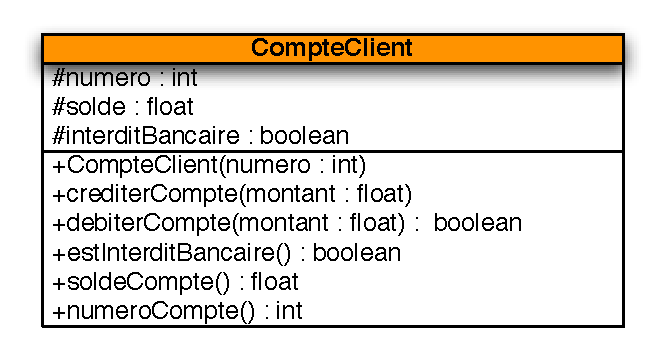
\includegraphics[scale=0.5]{fig/CompteClient.pdf}
    \end{center}
  \end{figure}
\vspace*{-6mm}
\begin{itemize}
	\item \emph{Encapsulation}: on a séparé les données des fonctions qui les manipulent, tout en conservant une seule entité, l'objet
	\item \emph{Protection}: on a protégé le {\tt solde}, dont la valeur ne peut être lue que par la méthode {\tt soldeCompte()}, et non modifiée\\ {\small sauf en ajoutant une méthode \textit{affecterCompte(x:float):void}.
}
\end{itemize}
\vspace*{-4mm}
\end{frame}

\begin{frame}{Exemple: La classe {\tt CompteClient} dans une banque (2/2)}
  \begin{figure}[htbp]
    \begin{center}
      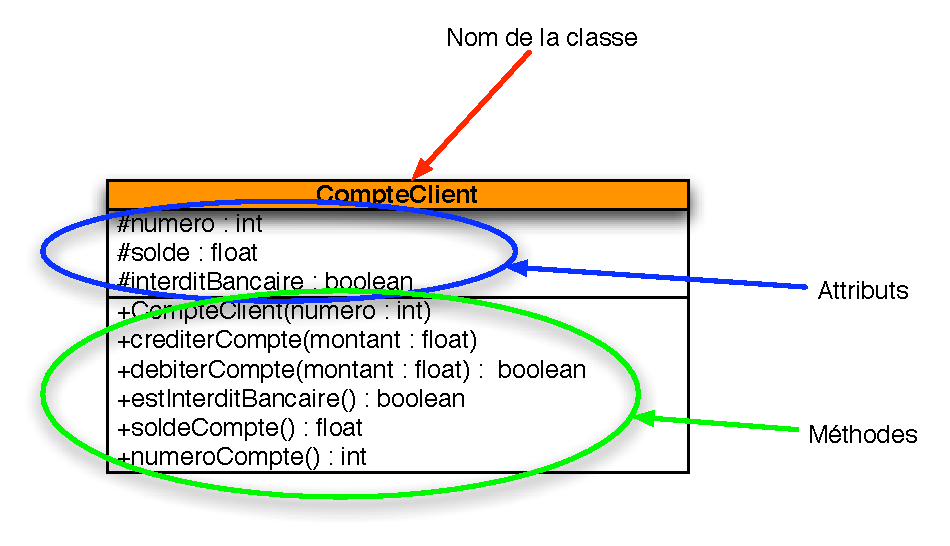
\includegraphics[scale=.4]{fig/CompteClientExplique.pdf}
    \end{center}
  \end{figure}

\end{frame}

% SSSSSSSSSSSSSSSSSSSSSSSSSSSSSSSSSSSSSSSSSSSSSS
\begin{frame}{Classes, instances...}
  \begin{figure}[htbp]
    \begin{center}
      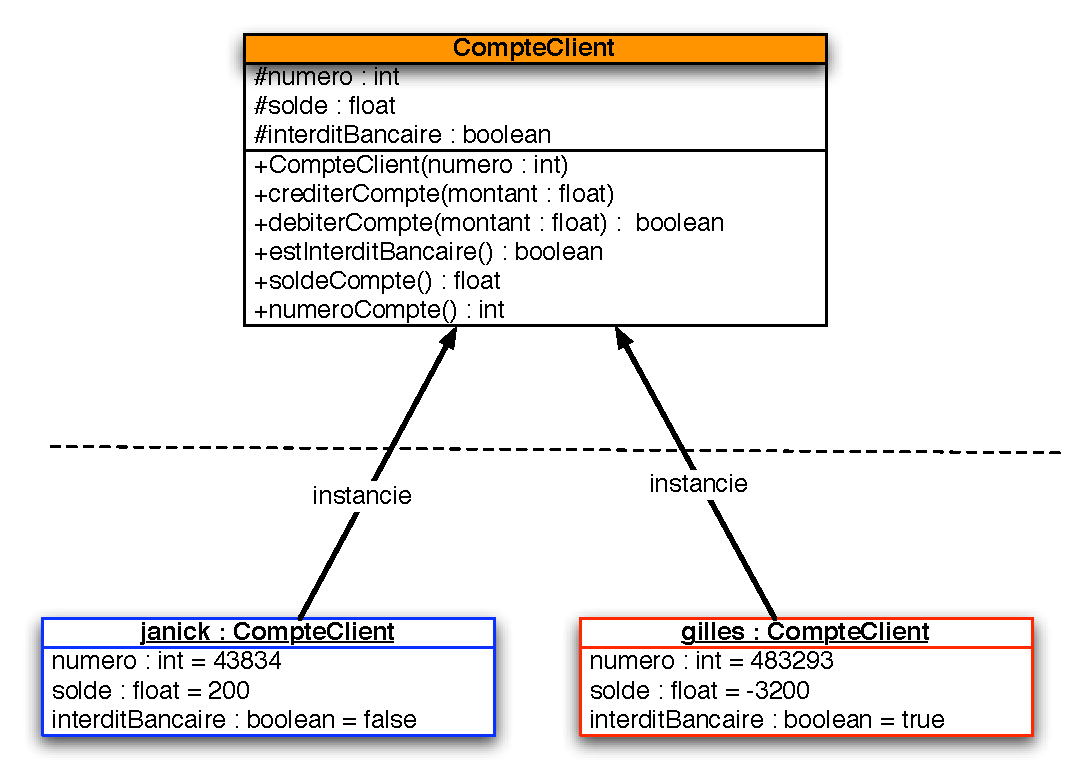
\includegraphics[scale=0.4]{fig/CompteClientInstance.pdf}
    \end{center}
  \end{figure}
\end{frame}

% constructeur & destructeur
%% cela pose d'autres questions : création et destruction d'un compte
\begin{frame}{Création d'un compte client}
\begin{itemize}
	\item Constat : on ne peut pas modifier le numéro d'un compte !
	\item la création d'un compte est une opération particulière qui doit :

\begin{itemize}
	\item définir de façon définitive le numéro du compte
	\item initialiser le solde du compte (à 0 généralement)
	\item mettre la variable \emph{interditBancaire} à faux
\end{itemize}
\item Les langages objet fournissent une méthode particulière : le \emph{constructeur}
\item Certains (dont C++) fournissent aussi un \emph{destructeur}
\end{itemize}
\end{frame}

\begin{frame}{Constructeurs et desctructeurs}
\begin{itemize}
\item Constructeur
\begin{itemize}
	\item Un constructeur est une fonction membre spéciale dont le nom est forcément celui de la classe
	\item Un constructeur n'a pas de type
	\item Une classe comporte généralement plusieurs constructeurs (en utilisant la surcharge, cf.  p.\ref{sec:surcharge})
	\item En fonction du nombre et du type des arguments passés, le constructeur approprié sera choisi
\end{itemize}
\item Destructeur
\begin{itemize}
\item Un destructeur est une fonction membre spéciale dont le nom est forcément un tilde ($\textasciitilde$) suivi du nom de la classe
\item Un destructeur n'a pas de type de retour ni d'argument
\end{itemize}
\end{itemize}
\end{frame}

\begin{frame}[fragile]
\frametitle{compte.h}
\begin{lstlisting}
#ifndef rvcpp_compte_h
#define rvcpp_compte_h

class compte {
private:
    float solde;
    bool ib;
    int numero;

public:
    float getSolde();
    int getNumero();

    void crediter(float montant);
    bool debiter(float montant);

    // constructeurs
    compte(int numero);

    // destructeur
    ~compte();
};

#endif
\end{lstlisting}
\end{frame}

\begin{frame}[fragile]
\frametitle{compte.cxx}
\begin{lstlisting}
#include "compte.h"

int compte::getNumero() {
    return numero;
}

float compte::getSolde() {
    return solde;
}

void compte::crediter(float montant) {
    solde += montant;
}

bool compte::debiter(float montant) {
    if (!ib && solde>=montant) {
        solde -= montant;
        return true;
    }
    return false;
}

compte::compte(int _numero) {
    numero = _numero;
    solde = 0.0;
    ib = false;
}

compte::~compte() {
    //nothing to do
}
\end{lstlisting}
\end{frame}

\begin{frame}[fragile]
\frametitle{Utilisation}
\begin{lstlisting}
#include <iostream>
using namespace std;

#include "compte.h"

int main() {
    compte janick(65136);
    janick.crediter(2000.0);
    cout << "solde du compte janick : " << janick.getSolde() << endl;
    if (janick.debiter(1000.0)) {
        cout << "debit autorise" << endl;
    }
    else {
        cout << "operation interdite" << endl;
    }
    cout << "solde du compte janick : " << janick.getSolde() << endl;
    compte *thomas = new compte(45558);
    thomas->crediter(500);
    cout << "solde du compte thomas : " << thomas->getSolde() << endl;
    delete thomas;
}
\end{lstlisting}
\pause\begin{block}{Résultat}
\tiny\begin{verbatim}
solde du compte janick : 2000
debit autorise
solde du compte janick : 1000
solde du compte thomas : 500
\end{verbatim}
\end{block}
\end{frame}

\begin{frame}{Rappels : encapsulation}
\begin{itemize}
\item Principe d'\textit{encapsulation} : tous les attributs d'une classe
doivent toujours être privés
\item Cela signifie que que seules les méthodes internes y ont accès (et donc qu'elles font les modifications comme il faut)
\item En clair : on a accès aux commandes de la voiture, pas directement à ce qu'il y a sous le capot
\item Ce n'est pas qu'un concept, c'est mis en \oe uvre et forcé par le langage
\begin{center}
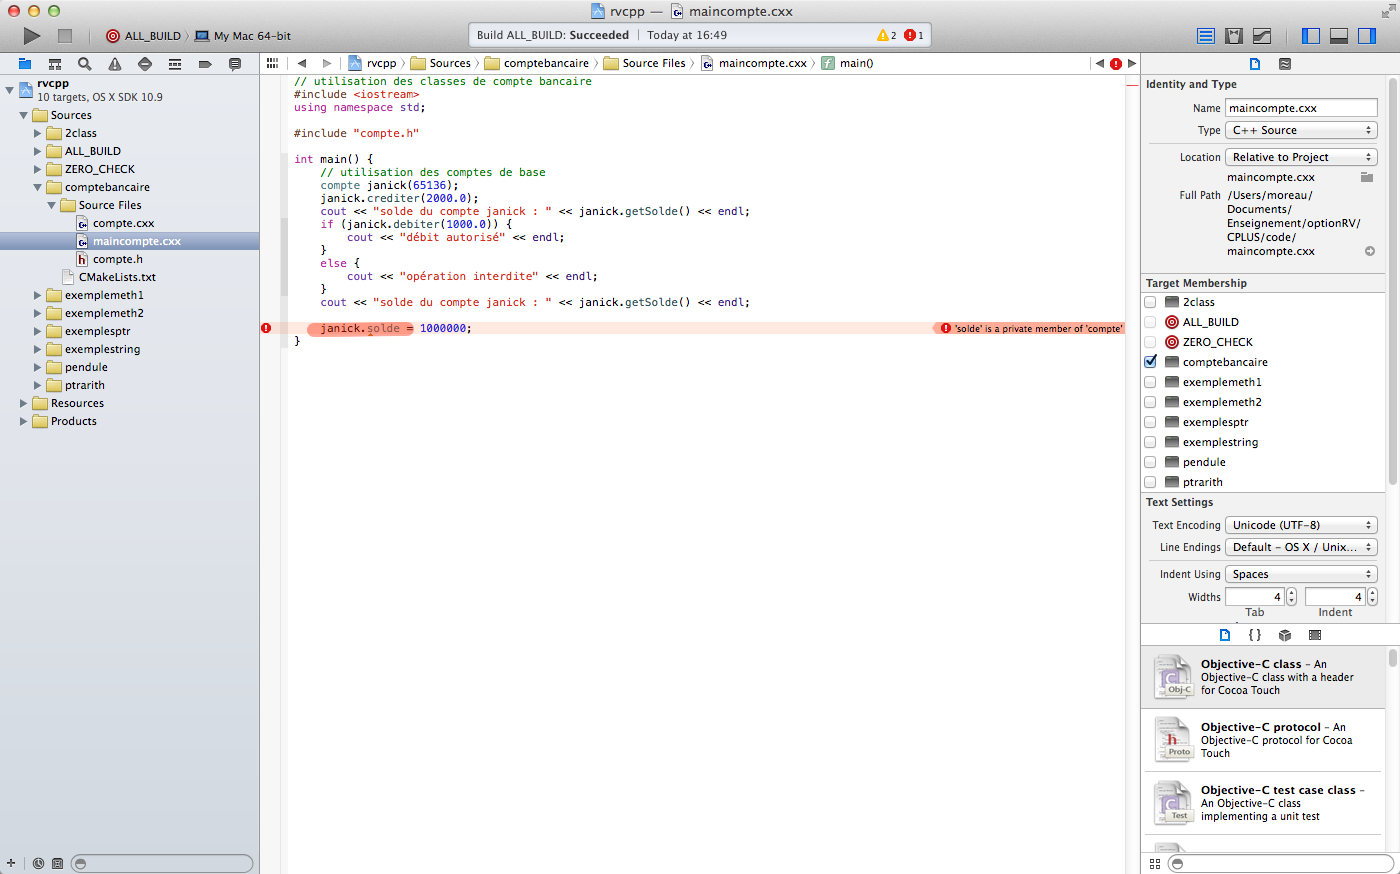
\includegraphics[width=\textwidth]{fig/encapsulation.png}
\end{center}
\end{itemize}
\end{frame}

\begin{frame}{Remarques}
\begin{itemize}
\item Nous reviendrons plus tard sur :
\begin{itemize}
\item Les protections
\item Les constructeurs et les destructeurs
\item La surcharge
\end{itemize}
\end{itemize}
\end{frame}

\begin{frame}[fragile]\frametitle{Interlude technique : les méthodes constantes}
\begin{itemize}
\item Une méthode constante est une méthode qui garantit ne pas altérer l'état d'un objet
\item On parle également de méthode en lecture seule
\item Déclaration :
\begin{itemize}
\item Le prototype de la méthode est suivi du mot-clé \texttt{const}
\item La déclaration de la méthode (dans le .cxx) est suivi de \texttt{const}, juste avant l'accolade de début
\end{itemize}
\item Utilité :
\begin{itemize}
\item Savoir ce que fait réellement une méthode (utilisation sans risque)
\item Optimisations du compilateur
\end{itemize}
\item Exemple : méthode \texttt{getSolde()} d'un compte bancaire
\begin{lstlisting}
float getSolde() const;

float compte::getSolde() const {
    return solde;
}
\end{lstlisting}
\end{itemize}
\end{frame}


% % Classes, mémoire et pointeurs

\begin{frame}[fragile]\frametitle{Gestion de la mémoire en C++ - les classes}

\begin{itemize}
\itemsep1pt\parskip0pt\parsep0pt
\item
  Que se passe-t-il lorsqu'une classe contient un élément d'un autre
  classe ?
\begin{lstlisting}
 class A {
 	B instB;
 };
\end{lstlisting}
\item
  En pratique l'instanciation de A créée automatiquement une instance de
  B dans la zone mémoire réservée pour l'instance de A.
\end{itemize}
\begin{columns}
\begin{column}{.6\textwidth}
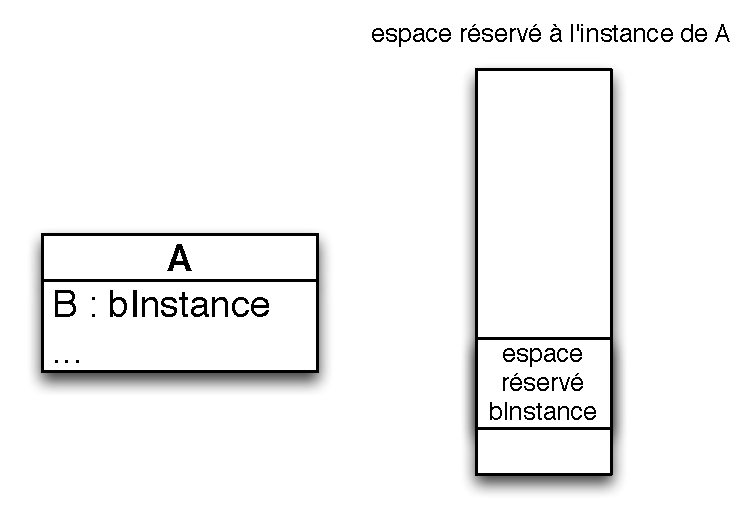
\includegraphics[width=6cm]{fig/inclusion-classe.pdf}
\end{column}
\begin{column}{.39\textwidth}
\begin{itemize}
\itemsep1pt\parskip0pt\parsep0pt
\item
  la destruction de A entraine la destruction de B
\end{itemize}
\end{column}
\end{columns}
\end{frame}


\begin{frame}[fragile]\frametitle{Gestion de la mémoire en C++ - les classes}

\begin{itemize}
\itemsep1pt\parskip0pt\parsep0pt
\item Utilisation d'un pointeur
\begin{lstlisting}
 class A {
 	B* instB;
 };
\end{lstlisting}
\item
  Les deux instances sont liées mais leur durée de vie est indépendante
\end{itemize}
\begin{columns}
\begin{column}{.6\textwidth}
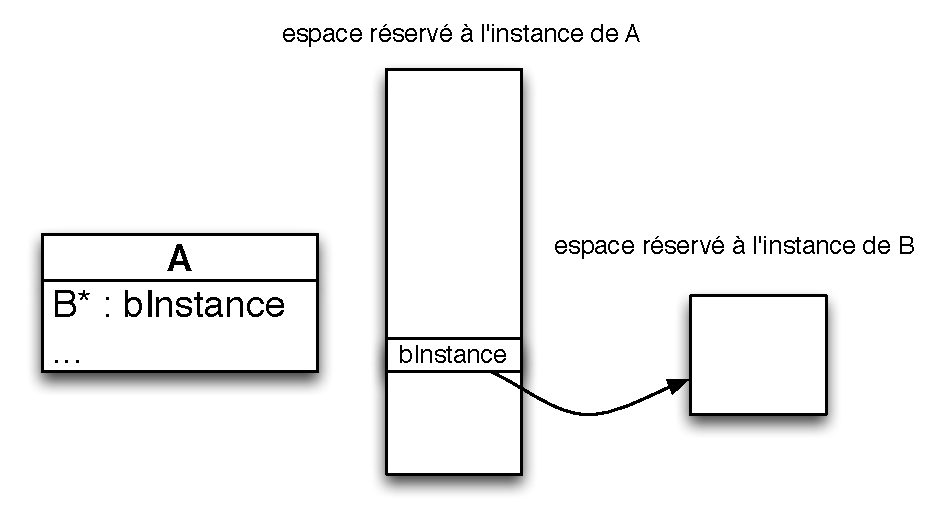
\includegraphics[width=6cm]{fig/inclusion-classeB.pdf}
\end{column}
\begin{column}{.39\textwidth}
\textbf{Exemple} de création/destruction de \textit{instB}

\begin{lstlisting}
A::A() {
	instB = new B();
}

A::~A() {
	delete instB;
}
\end{lstlisting}
\end{column}
\end{columns}
\end{frame}

\begin{frame}{Questions ?}

\begin{itemize}
\itemsep1pt\parskip0pt\parsep0pt
\item
  Pourquoi avoir écrit \textbf{exemple} au transparent précédent ?
\item
  Cycle de vie d'un objet vs un autre

  \begin{itemize}
  \itemsep1pt\parskip0pt\parsep0pt
  \item
    une question de génie de logiciel : B a-t-il une raison de survivre
    à A ?

    \begin{itemize}
    \itemsep1pt\parskip0pt\parsep0pt
    \item
      non : bouton appartenant à une fenêtre
    \item
      oui : un objet qui change de propriétaire (analogie jeu vidéo : un
      objet ramassé puis relâché)
    \end{itemize}
  \end{itemize}
\item
  Ok, mais C++ ne sait pas se débarrasser d'un objet tout seul

  \begin{itemize}
  \itemsep1pt\parskip0pt\parsep0pt
  \item
    Surtout si on utilise des pointeurs et des références
  \item
    On \textbf{doit} avoir une stratégie de gestion de la mémoire

    \begin{itemize}
    \itemsep1pt\parskip0pt\parsep0pt
    \item
      éviter l'utilisation de mémoire sans raison
    \item
      éviter d'utiliser un objet préalablement libéré
    \end{itemize}
  \item
    Cas typique : dans un contexte de gestion dynamique de la mémoire,
    on a une fonction qui retourne un objet

    \begin{itemize}
    \itemsep1pt\parskip0pt\parsep0pt
    \item
      qui se charge de l'allocation mémoire ? l'appelant, l'appelé ?
    \item
      qui est responsable de la libération de la mémoire ?
    \item
      attention aux créations d'objets temporaires
    \end{itemize}
  \end{itemize}
\end{itemize}

\end{frame}

\subsection{La surcharge}
\label{sec:surcharge}

\begin{frame}{Surcharge et redéfinition en C++}

\begin{itemize}
\itemsep1pt\parskip0pt\parsep0pt
\item
  principe : des fonctions qui portent le même nom
\item
  \textbf{surcharge} : plusieurs fonctions qui portent le même nom mais
  qui n'ont pas les mêmes paramètres (en nombre et/ou en type)

  \begin{itemize}
  \itemsep1pt\parskip0pt\parsep0pt
  \item
    le compilateur décide de la fonction à appeler en fonction du type
    des paramètres
  \item
    exemple : des fonctions \textit{max()} à respectivement 2, 3 ou 4 paramètres, des fonctions \textit{max()} s'appliquant à des types différents
  \item
    Cas particulier : surcharge des opérateurs
  \end{itemize}
\item
  \textbf{redéfinition} : plusieurs fonctions qui portent le nom et qui
  ont les mêmes paramètres

  \begin{itemize}
  \itemsep1pt\parskip0pt\parsep0pt
  \item
    utilisé plus tard pour l'héritage
  \end{itemize}
\end{itemize}

\end{frame}

\begin{frame}[fragile]\frametitle{Surcharge de fonctions}

\begin{itemize}
\itemsep1pt\parskip0pt\parsep0pt
\item
  Exemple : des fonctions qui calculent le maximum de plusieurs entiers
\item
  Ecriture ``C'' : une fonction \emph{max2(a,b)} , une fonction
  \emph{max3(a,b,c)}\ldots{}
\item
  Ecriture ``C++'' : toujours le même nombre de fonctions, mais elles
  portent toutes le même nom
\end{itemize}
\begin{lstlisting}
int max(int a,int b) {
    if (a>b) {
        return a;
    }
    else {
        return b;
    }
}

int max(int a,int b, int c) {
    return max(a,max(b,c));
}

int max(int a,int b, int c,int d) {
    return max(max(a,b),max(c,d));
}

int main() {
    cout << "max(2,4) = " << max(2,4) << endl;
    cout << "max(2,4,3) = " << max(2,4,3) << endl;
    cout << "max(6,4,5,7) = " << max(6,4,5,7) << endl;
}
\end{lstlisting}
\end{frame}

\begin{frame}{Cas particulier : surcharge des opérateurs}
\begin{itemize}
\item Les opérateurs sont des fonctions !
\begin{itemize}
\item Exemple : l'opérateur (binaire) d'addition est une fonction surchargée à deux paramètres de type \textit{t} et qui retourne un type \textit{t}
\item Elle pourrait s'écrire \texttt{int add(int a,int b)}
\item Inversement, une fonction de comparaison entre deux objets de type \textit{C} s'écrit \texttt{bool egalO(C const\& a, C const\&b)}
\item Autre possibilité, sous forme de méthode de la classe \textit{C} : \texttt{bool egal(const O\&a)}
\item On aimerait pouvoir l'écrire avec l'opérateur \texttt{==}
\end{itemize}
\end{itemize}
\end{frame}

\begin{frame}[fragile]\frametitle{Exemple : comparaison de deux nombres complexes}
\begin{itemize}
\item Déclaration des opérateurs (syntaxe forcée par la suite)
\begin{lstlisting}
class complexe1 {
private:
    double re;
    double im;

public:
...
    bool egal(complexe1 const& c1) const;
};

// operateurs externes
bool egal(complexe1 const&a,complexe1 const&b);
\end{lstlisting}
\item Définition
\begin{lstlisting}
bool complexe1::egal(complexe1 const& c1) const {
    if (re == c1.re && im == c1.im) {
        return true;
    }
    else {
        return false;
    }
}

bool egal(complexe1 const&a,complexe1 const&b) {
    return a.egal(b);
}
\end{lstlisting}
\end{itemize}
\end{frame}

\begin{frame}[fragile]\frametitle{Utilisation des fonctions}
\begin{itemize}
\item Code de test
\begin{lstlisting}
int main() {
    complexe1 c1,c2(2,3),c3(c2);
    cout << "c1 == c2 (interne) " << c1.egal(c2) << endl;
    cout << "c1 == c2 (externe) " << egal(c1,c2) << endl;
    cout << "c3 == c2 (interne) " << c3.egal(c2) << endl;
    cout << "c3 == c2 (externe) " << egal(c3,c2) << endl;

}
\end{lstlisting}
\begin{block}{Résultat}
{\tiny
\begin{verbatim}
c1 == c2 (interne) 0
c1 == c2 (externe) 0
c3 == c2 (interne) 1
c3 == c2 (externe) 1
\end{verbatim}
}
\end{block}
\item Comment écrire \texttt{c1 == c2} ?
\begin{itemize}
\item Utilisation d'un nouveau mot-clé : \texttt{operator}
\item La fonction associée à un opérateur \texttt{==} est \texttt{operator==()}
\end{itemize}
\end{itemize}
\end{frame}

\begin{frame}[fragile]\frametitle{Surcharge de l'opérateur \texttt{==}}
\begin{itemize}
\item Déclaration
\begin{lstlisting}
bool operator==(complexe1 const&a,complexe1 const&b);
\end{lstlisting}
\item Définition
\begin{lstlisting}
bool operator==(complexe1 const&a,complexe1 const&b) {
    return a.egal(b);
}
\end{lstlisting}
\item Utilisation
\begin{lstlisting}
    cout << "c1 == c2 (==) " << (c1 == c2) << endl;
    cout << "c3 == c2 (==) " << (c3 == c2) << endl;
\end{lstlisting}
\begin{block}{Résultat}
{\tiny
\begin{verbatim}
c1 == c2 (==) 0
c3 == c2 (==) 1
\end{verbatim}
}
\end{block}
\item A vous de faire de même avec l'opérateur \texttt{!=}
\end{itemize}
\end{frame}

\begin{frame}[fragile]\frametitle{Surcharge de l'opérateur \texttt{!=}}
\begin{itemize}
\item Déclaration
\begin{lstlisting}
bool operator!=(complexe1 const&a,complexe1 const&b);
\end{lstlisting}
\item Définition
\begin{lstlisting}
bool operator!=(complexe1 const&a,complexe1 const&b) {
    return !a.egal(b);
}
\end{lstlisting}
\item Utilisation
\begin{lstlisting}
    cout << "c1 != c2 " << (c1 != c2) << endl;
    cout << "c3 != c2 " << (c3 != c2) << endl;
\end{lstlisting}
\begin{block}{Résultat}
{\tiny
\begin{verbatim}
c1 != c2 1
c3 != c2 0
\end{verbatim}
}
\end{block}
\item Remarques
\begin{itemize}
\item Pourquoi avoir réutilisé le code existant ?
\item Fonction externe et encapsulation...
\end{itemize}
\end{itemize}
\end{frame}

\begin{frame}[fragile]\frametitle{Le cas de l'addition}
\begin{itemize}
\item Idée \textit{naturelle}
\begin{lstlisting}
complexe1 operator+(complexe1 const&c1,complexe1 const&c2);
\end{lstlisting}
\item Implémentation
\begin{itemize}
\item encapsulation = pas d'accès direct aux variables membres, lourdeur syntaxique
\item passer par une fonction \textit{amie} : rupture du principe d'encapsulation
\item passer par une méthode
\begin{itemize}
\item Soit par délégation
\item Soit par analogie avec l'opérateur unaire : \texttt{a += 5}
\item Une approche véritablement objet
\end{itemize}
\end{itemize}
\end{itemize}
\end{frame}

\begin{frame}[fragile]\frametitle{Surcharge de l'opérateur \texttt{+=}}
\begin{itemize}
\item Déclaration
\begin{lstlisting}
    void operator+=(complexe1 const&c1);
\end{lstlisting}
\item Définition
\begin{lstlisting}
void complexe1::operator+=(complexe1 const&c1) {
    re += c1.re;
    im += c1.im;
}
\end{lstlisting}
\item Utilisation
\begin{lstlisting}
    c2 += c3;
\end{lstlisting}
\begin{block}{Résultat}
{\tiny
\begin{verbatim}
2+3i + 2+3i = 4+6i
\end{verbatim}
}
\end{block}
\item Remarques
\begin{itemize}
\item Pour bien faire, l'opérateur devrait retourner un \texttt{complexe1\&}
\item Utilisation de \texttt{this}
\end{itemize}
\end{itemize}
\end{frame}

\begin{frame}[fragile]\frametitle{Surcharge de l'opérateur \texttt{+}}
\begin{itemize}
\item Déclaration
\begin{lstlisting}
complexe1 operator+(complexe1 const& c1,complexe1 const& c2);
\end{lstlisting}
\item Définition
\begin{lstlisting}
complexe1 operator+(complexe1 const& c1,complexe1 const &c2) {
    complexe1 c3(c1);
    c3 += c2;
    return c3;
}
\end{lstlisting}
\item Utilisation
\begin{lstlisting}
    c = a+b;
    t = t1+t2+t3;
\end{lstlisting}
\begin{block}{Résultat}
{\tiny
\begin{verbatim}
3+4i + 3+2i = 6+6i
23+3i + 3+5i + 2+1i = 28+9i
\end{verbatim}
}
\end{block}
\item A vous de jouer : ajout d'un complexe et d'un réel !
\end{itemize}
\end{frame}

\begin{frame}{Autres opérateurs surchargeables}

\begin{itemize}
\itemsep1pt\parskip0pt\parsep0pt
\item
  opérateurs mathématiques

  \begin{itemize}
  \itemsep1pt\parskip0pt\parsep0pt
  \item
    opérateurs binaires : +,-,*,/,\%
  \item
    opérateurs unaires : +=,-=,*=,/=,\%=
  \end{itemize}
\item
  opérateurs logiques

  \begin{itemize}
  \itemsep1pt\parskip0pt\parsep0pt
  \item
    bits à bits : \^{}, \textbar{}, \&, \textasciitilde{},
    \textless{}\textless{}, \textgreater{}\textgreater{} (et leur
    version unaire)
  \item
    relationnels : ==, !=, \textless{}, \textgreater{}, \textless{}=,
    \textgreater{}=
  \item
    logiques : !, \&\&, \textbar{}\textbar{}
  \end{itemize}
\item
  mais aussi

  \begin{itemize}
  \itemsep1pt\parskip0pt\parsep0pt
  \item
    opérateur d'affectation =
  \item
    opérateur d'accès tableau {[}{]}
  \item
    opérateur d'appel de fonction ()
  \item
    opérateur de gestion des adresses : \&, * et -\textgreater{}
  \end{itemize}
  \item Certains sont plus dangereux que d'autres...
\end{itemize}

\end{frame}

\begin{frame}{Autres opérateurs surchargeables (suite)}

\begin{itemize}
\itemsep1pt\parskip0pt\parsep0pt
\item
  Les opérateurs de gestion de mémoire (new, new{[}{]}, delete,
  delete{[}{]})
\item
  l'opérateur de séparation d'une liste , (utilité ??)
\item
  les opérateurs de conversion
\item
  Certains opérateurs ne \textbf{peuvent (quand même) pas} être
  surchargés

  \begin{itemize}
  \itemsep1pt\parskip0pt\parsep0pt
  \item
    l'opérateur ternaire ? :
  \item
    sélection d'un membre ., .*
  \item
    opérateur de résolution de portée ::
  \item
    \texttt{sizeof}
  \item
    \texttt{typeid}
  \end{itemize}
\item
  De façon générale, la surcharge des opérateurs est à utiliser

  \begin{itemize}
  \itemsep1pt\parskip0pt\parsep0pt
  \item
    avec parcimonie (on ne travaille pas tout seul)
  \item
    pour l'extension des opérations communes à de nouveaux types
  \item
    avec la même sémantique qu'avant la surcharge

    \begin{itemize}
    \itemsep1pt\parskip0pt\parsep0pt
    \item
      typiquement ne pas transformer un + en - !
    \end{itemize}
  \end{itemize}
\end{itemize}

\end{frame}

\begin{frame}[fragile]
\frametitle{Cas particulier intéressant : surcharge de l'opérateur
\texttt{\textless{}\textless{}}}

\begin{itemize}
\itemsep1pt\parskip0pt\parsep0pt
\item
  Pourquoi faire ?

  \begin{itemize}
  \itemsep1pt\parskip0pt\parsep0pt
  \item
    afficher des infos relatives à un objet qu'on a défini

    \begin{itemize}
    \itemsep1pt\parskip0pt\parsep0pt
    \item
      via un simple \texttt{cout} par exemple
    \end{itemize}
  \item
    sauver (et plus tard recharger) à partir d'un fichier
  \end{itemize}
\item
  Comment ?

  \begin{itemize}
  \itemsep1pt\parskip0pt\parsep0pt
  \item
    Plus tard : gestion des flux en C++
  \item
    Maintenant : surcharge simple et utilisation avec \texttt{cout}
  \item
    \texttt{\textless{}\textless{}} est bien un opérateur : ostream\&
    \texttt{operator\textless{}\textless{}(ostream\&,\emph{type} const\&)}
  \end{itemize}
\item
  Redéfinition pour le type complexe
\end{itemize}
\begin{lstlisting}
ostream& operator<<(ostream&s,complexe1 const&c) {
    s << c.getRe() << "+" << c.getIm() << "i";
    return s;
}
\end{lstlisting}
\end{frame}


\subsection{L'héritage en C++}


%%%%%%%%%%%%%%%%%%%%%%%%%%%%%%%%%%%%%%%%%%%%%%
\begin{frame}{Rappels : les classes}
\begin{itemize}
	\item Une classe représente une <<famille>> d'objets partageant les mêmes propriétés et méthodes
	\item Une classe sert à définir les propriétés des objets d'un type donné
	\begin{itemize}
		\item décrit l'ensemble des données et des opérations sur ces données
		\item elle sert de modèle pour la création d'objets (instances de la classe)
	\end{itemize}
\end{itemize}
\end{frame}

%%%%%%%%%%%%%%%%%%%%%%%%%%%%%%%%%%%%%%%%%%%%%%
\begin{frame}{Réutilisation : introduction}
\begin{itemize}
	\item Comment utiliser une classe comme une brique de base pour concevoir d'autres objets ?
	\item En conception objet, on définit des associations (relations) entre objets pour définir la réutilisation entre classes
	\item UML (Unified Modeling Language) définit toute une terminologie des associations possibles entre classes
	\begin{itemize}
		\item un des objectifs d'un cours de <<Génie Logiciel>> (option info par exemple)
		\item un objet fait appel à un autre $\longrightarrow$ délégation
		\item un objet peut être créé à partir d'un autre objet $\longrightarrow$ héritage
	\end{itemize}
\end{itemize}
\end{frame}

\subsection{Délégation}
\subsubsection*{Exemple}

%%%%%%%%%%%%%%%%%%%%%%%%%%%%%%%%%%%%%%%%%%%%%%
\begin{frame}[fragile]
\frametitle{Délégation}
\begin{itemize}
	\item Un objet \texttt{o1} membre de la classe \emph{C1} utilise les services d'un objet \texttt{o2} instance de la classe \emph{C2} (\texttt{o1} délègue une partie de son activité à \texttt{o2})
	\item La classe \emph{C1} utilise les services de la classe \emph{C2}
\begin{figure}[htbp]
    \begin{center}
      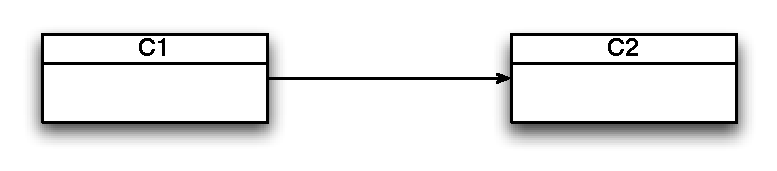
\includegraphics[scale=.5]{fig/delegation.pdf}
    \end{center}
  \end{figure}
  \item La classe cliente (\emph{C1}) utilise les services de la classe serveuse
\end{itemize}
\begin{block}{Schéma type}
\begin{lstlisting}[language=C++]
public class C1 {
private:
   C2 o2; // ou C2 *o2;
\end{lstlisting}
\end{block}
\end{frame}

%%%%%%%%%%%%%%%%%%%%%%%%%%%%%%%%%%%%%%%%%%%%%%
\begin{frame}[fragile]
\frametitle{Délégation : exemple}
\begin{itemize}
  \item Exemple de la classe \emph{Cercle}
  \begin{itemize}
  	\item rayon : un nombre réel
	\item centre : deux réels ou bien un \emph{Point}
  \end{itemize}
\end{itemize}
\begin{lstlisting}[language=C++]
public class Cercle {
private:
  Point centre; // ou Point *centre
  private double rayon;

public:
  Cercle(Point _centre, double _rayon) {
    centre = _centre;
    rayon = _rayon;
  }
};
\end{lstlisting}
\end{frame}

%%%%%%%%%%%%%%%%%%%%%%%%%%%%%%%%%%%%%%%%%%%%%%
\begin{frame}[fragile]
\frametitle{Délégation : exemple}
\begin{itemize}
	\item l'association entre les classes \emph{Cercle} et \emph{Point} exprime le fait qu'un cercle \textbf{possède} (a un) centre
	\item Le point représentant le centre a une existence autonome (cycle de vie indépendant
	\item Il peut être utilisé en dehors du cercle dont il est le centre !
	\begin{itemize}
		\item si on translate le cercle, on translate le point et tous les objets qui utilisent ce point
		\item Solution (en place) : effectuer une copie du point dans le constructeur
	\end{itemize}
\begin{lstlisting}[language=C++]
// cas Point centre
  centre = _centre; // dans les deux cas
// cas Point *centre
  centre = new Point(_centre);
\end{lstlisting}
%% note : les cycles de vie du cercle et du point sont maintenant liés : si le cercle est déplacé ou déruit
%% le point l'est aussi
\end{itemize}
\end{frame}

\subsubsection*{Agrégation / Composition}

%%%%%%%%%%%%%%%%%%%%%%%%%%%%%%%%%%%%%%%%%%%%%%
\begin{frame}{Agrégation / Composition}
\begin{itemize}
	\item L'exemple précédent traduit deux nuances (sémantiques) de l'association \textbf{a un} entre la classe \emph{Cercle} et la classe \emph{Point}
	\item UML distingue deux types de sémantique en définissant deux types de relations
\end{itemize}
\begin{figure}[htbp]
    \begin{center}
      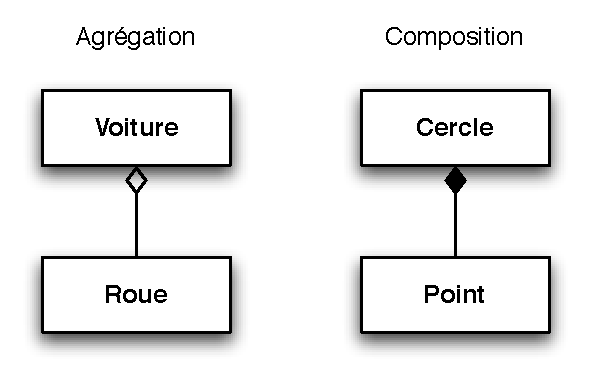
\includegraphics[scale=.45]{fig/agregcompo.pdf}
    \end{center}
  \end{figure}
\end{frame}

%%%%%%%%%%%%%%%%%%%%%%%%%%%%%%%%%%%%%%%%%%%%%%
\begin{frame}{Agrégation / Composition}
\begin{itemize}
	\item \textbf{Agrégation} : l'élément agrégé \emph{Roue} a un existence autonome en dehors de l'agrégat
	\item \textbf{Agrégation forte / composition} : à un même moment, une instance de composant \emph{Point} ne peut être liée qu'à un seul agrégat \emph{Cercle} et le composant a un cycle de vie dépendant de l'agrégat
	\begin{itemize}
	\item Pas vrai dans tous les cas, mais voulu et forcé ici !
	\end{itemize}
\end{itemize}
\end{frame}

\subsubsection*{Syntaxe}

%%%%%%%%%%%%%%%%%%%%%%%%%%%%%%%%%%%%%%%%%%%%%%
\begin{frame}{Héritage : exemple introductif}
\begin{itemize}
	\item Le problème :
	\begin{itemize}
		\item une application a besoin de services dont une partie seulement est proposée par une classe déjà définie
		\item ne pas réécrire le code
	\end{itemize}
\end{itemize}
\begin{figure}[htbp]
    \begin{center}
      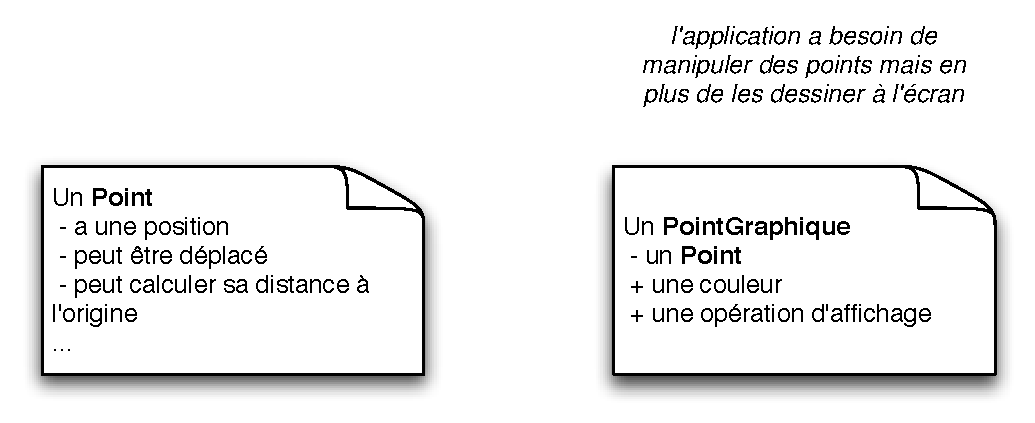
\includegraphics[scale=.42]{fig/pointgraphique.pdf}
    \end{center}
  \end{figure}
\end{frame}

%%%%%%%%%%%%%%%%%%%%%%%%%%%%%%%%%%%%%%%%%%%%%%
\begin{frame}{Pourquoi l'héritage plutôt que agrégation/composition ?}
\begin{itemize}
	\item par simplicité...
	\item ici, on réutilise les méthodes de {Point} dans {PointGraphique}
	\item éviter de rerouter tous les appels à \textit{deplacer()} de {PointGraphique} vers {Point}
	\item exemple opposé : création d'une pile à partir d'une liste
	\begin{itemize}
		\item on ne veut pas donner accès à toutes les méthodes de la liste
	\end{itemize}
\end{itemize}
\end{frame}

%%%%%%%%%%%%%%%%%%%%%%%%%%%%%%%%%%%%%%%%%%%%%%
\begin{frame}[fragile]
\frametitle{Héritage : syntaxe C++}
\begin{itemize}
	\item La classe \emph{PointGraphique} hérite de (elle étend) la classe \emph{Point}
	\begin{itemize}
		\item elle possède les variables et méthodes définies dans la classe \emph{Point} ($x$ et $y$)
		\item elle ajoute des attributs de couleur \texttt{r,g,b}
		\item elle définit une nouvelle méthode \texttt{dessine()}
	\end{itemize}
\end{itemize}
\begin{exampleblock}{Déclaration}
\begin{lstlisting}[language=C++]
class PointGraphique : public Point {
private:
    int r,g,b;

public:
    PointGraphique();
    PointGraphique(double _x,double _y,int _r,int _g, int _b);
    PointGraphique(double _x,double _y);

    void dessine();
};
\end{lstlisting}
\end{exampleblock}
\end{frame}

\begin{frame}[fragile]
\frametitle{Héritage : Ecriture des méthodes}
\begin{itemize}
	\item Seul le constructeur diffère !
	\item Il peut (doit) faire appel au constructeur de la classe \textit{Point}
	\item Syntaxe \texttt{\textit{Pointgraphique::PointGraphique( ) : Point( )}}
\end{itemize}
\begin{exampleblock}{Définition des méthodes}
\begin{lstlisting}[language=C++]
#include "point.h"
#include "pointgraphique.h"

PointGraphique::PointGraphique() : Point() {
    r = g = b = 255; // couleur par defaut = blanc
}

PointGraphique::PointGraphique(double _x,double _y,int _r,int _g, int _b)
 : Point(_x,_y), r(_r), g(_g), b(_b) {
    // plus rien a faire
}

PointGraphique::PointGraphique(double _x,double _y) : Point(_x,_y) {
    r = g = b = 255; // couleur par defaut = blanc
}
\end{lstlisting}
\end{exampleblock}
\end{frame}

%%%%%%%%%%%%%%%%%%%%%%%%%%%%%%%%%%%%%%%%%%%%%%%
\begin{frame}[fragile]
\frametitle{Utilisation des instances d'une classe héritée}
\begin{itemize}
	\item Un objet instance de \emph{PointGraphique} possède les attributs définis dans \emph{PointGraphique} ainsi que ceux définis dans \emph{Point}
	\item Un  objet instance de \emph{PointGraphique} répond aux messages définis par les méthodes décrites dans \emph{PointGraphique} et aussi à ceux définis dans les méthodes de \emph{Point}
\end{itemize}
\begin{exampleblock}{Utilisation}
\begin{lstlisting}[language=C++]
int main() {
    PointGraphique pg;

    pg.setX(5.5);
    pg.setY(2.3);
    pg.translater(2.0, 0.0);
    pg.setCouleur(128, 128, 0);

}
\end{lstlisting}
\end{exampleblock}
\end{frame}

%%%%%%%%%%%%%%%%%%%%%%%%%%%%%%%%%%%%%%%%%%%%%%%
\begin{frame}[fragile]
\frametitle{Résolution statique des messages}
\begin{figure}[htbp]
    \begin{center}
      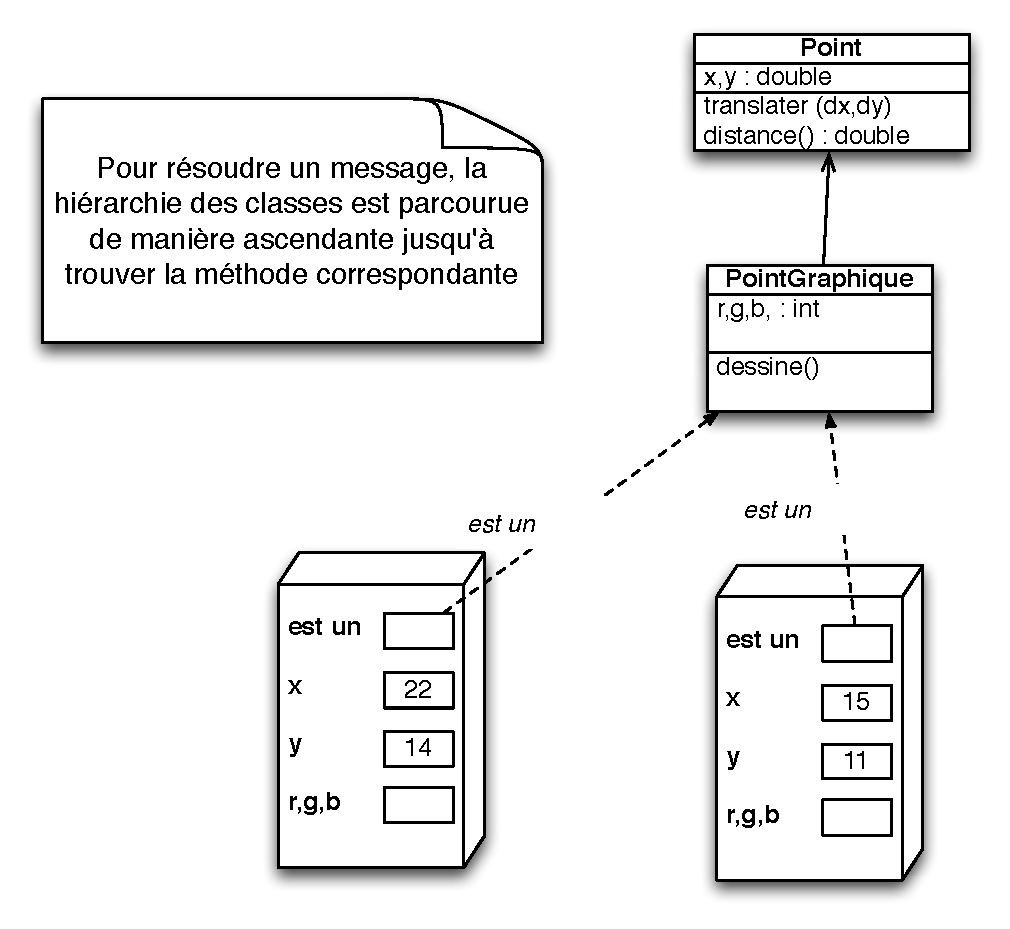
\includegraphics[scale=.42]{fig/resolution.pdf}
    \end{center}
  \end{figure}
\end{frame}

\subsubsection*{Terminologie}

%%%%%%%%%%%%%%%%%%%%%%%%%%%%%%%%%%%%%%%%%%%%%%
\begin{frame}{Terminologie de l'héritage}
\begin{itemize}
	\item L'\textbf{héritage} permet de reprendre les caractéristiques d'une classe $M$ existante pour les étendre et définir ainsi une nouvelle classe $F$ qui hérite de $M$
	\item les objets de $F$ possèdent toutes les caractéristiques de $M$ avec en plus celles définies dans $F$
	\begin{itemize}
		\item $M$ est la classe mère et $F$ la classe fille
		\item $F$ hérite de $M$
		\item $F$ est une sous-classe de $M$
		\item $M$ est la super-classe de $F$
	\end{itemize}
\end{itemize}
\end{frame}

%%%%%%%%%%%%%%%%%%%%%%%%%%%%%%%%%%%%%%%%%%%%%%
\begin{frame}{Généralisation / spécialisation}
\begin{figure}[htbp]
    \begin{center}
      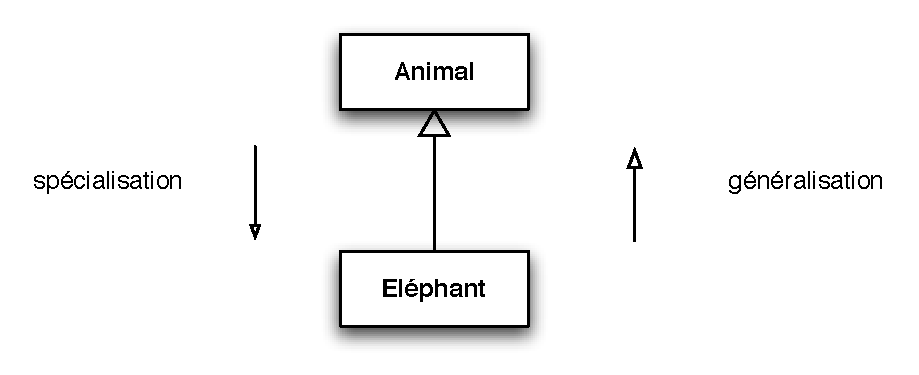
\includegraphics[scale=.45]{fig/genspe.pdf}
    \end{center}
  \end{figure}
\begin{itemize}
	\item la \textbf{généralisation} exprime la relation <<est-un>> entre une classe et sa super-classe
	\item la \textbf{spécialisation} exprime la relation de <<particularisation>> entre une classe et sa sous-classe
\end{itemize}
\end{frame}

%%%%%%%%%%%%%%%%%%%%%%%%%%%%%%%%%%%%%%%%%%%%%%%
\begin{frame}{Généralisation / spécialisation}
\begin{itemize}
	\item Utilisation de la spécialisation : \textbf{réutilisation} par modification incrémentielle des descriptions existantes
	\item Utilisation de la généralisation : \textbf{abstraction} par factorisation des propriétés communes aux sous-classes
	\item il n'y a pas de limitation dans le nombre de niveaux de la hiérarchie d'héritage
	\item les méthodes et les attributs sont automatiquement héritées au travers de tous les niveaux
\end{itemize}
\end{frame}

%\subsection{Redéfinition des méthodes}

%%%%%%%%%%%%%%%%%%%%%%%%%%%%%%%%%%%%%%%%%%%%%%
\begin{frame}{Redéfinition des méthodes}
\begin{itemize}
	\item une sous-classe peut \textbf{redéfinir} des méthodes dont elle hérite et fournir ainsi des implémentations spécialisées pour celles-ci
	\item lorsque la classe définit une méthode dont le nom, le type de retour et les arguments sont identiques à ceux d'une méthode dont on hérite
	\begin{itemize}
	\item On dit aussi qu'une méthode \textbf{masque} celle de la classe mère
	\end{itemize}
	\item Lorsqu'une méthode redéfinie par une classe est invoquée pour un objet de cette classe, c'est la nouvelle définition qui est invoquée
\end{itemize}
\end{frame}

%%%%%%%%%%%%%%%%%%%%%%%%%%%%%%%%%%%%%%%%%%%%%%%
\begin{frame}[fragile]
\frametitle{{\href{code/exheritageA.cxx}{\scalebox{.25}{
\includegraphics{fig/codeicon}}}} Redéfinition des méthodes : exemple (1/2)}
\begin{itemize}
\item Déclaration
\begin{lstlisting}[language=C++]
class exheritageA {
public:
    void hello();
    void affiche();

};

class exheritageB : public exheritageA {
public:
    void affiche();
};
\end{lstlisting}
\item Définition
\begin{lstlisting}
void exheritageA::hello() {
    cout << "hello" << endl;
}

void exheritageA::affiche() {
    cout << "je suis un objet de la classe exheritageA" << endl;
}

void exheritageB::affiche() {
    cout << "je suis un objet de la classe exheritageB" << endl;
}
\end{lstlisting}
\end{itemize}
\end{frame}
%
%%%%%%%%%%%%%%%%%%%%%%%%%%%%%%%%%%%%%%%%%%%%%%%
\begin{frame}[fragile,containsverbatim]
\frametitle{{\href{code/exheritageB.java}{\scalebox{.25}{
\includegraphics{fig/codeicon}}}}  Redéfinition des méthodes : exemple (2/2)}
\begin{lstlisting}[language=C++]
int main() {
    exheritageA a;
    exheritageB b;

    a.hello();
    b.hello();

    a.affiche();
    b.affiche();
}
\end{lstlisting}
\begin{itemize}
	\item produit l'affichage suivant
\end{itemize}
\pause \begin{block}{Résultat}
{\tiny \begin{verbatim}
hello
hello
je suis un objet de la classe exheritageA
je suis un objet de la classe exheritageB
\end{verbatim}}
\end{block}
\end{frame}
%
%
%%%%%%%%%%%%%%%%%%%%%%%%%%%%%%%%%%%%%%%%%%%%%%%
\begin{frame}{Redéfinition des méthodes}
\begin{itemize}
	\item Ne pas confondre redéfinition et surcharge !
\end{itemize}
\begin{figure}[htbp]
    \begin{center}
      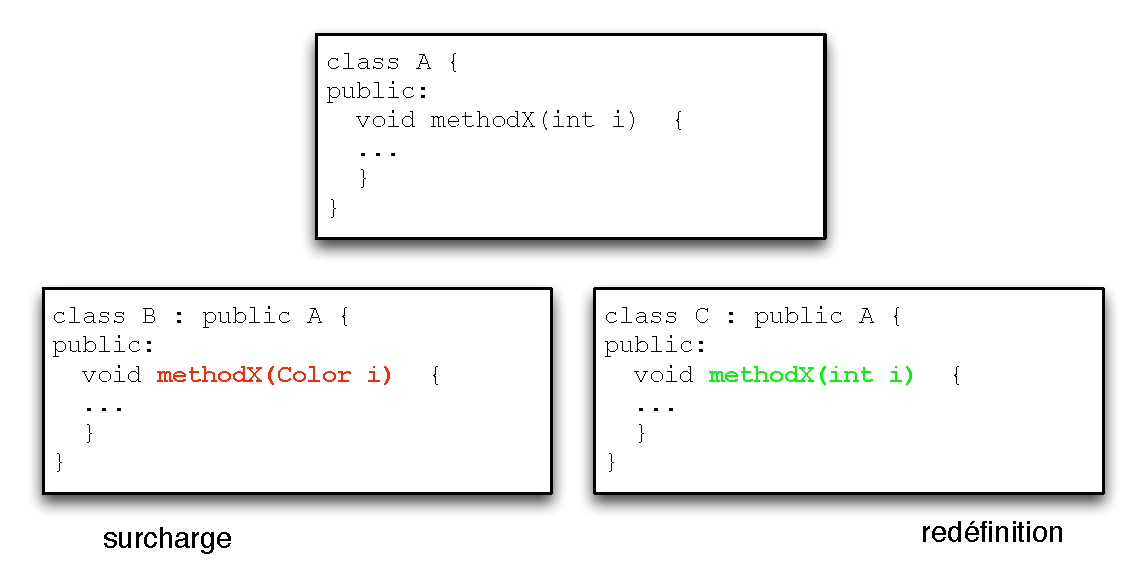
\includegraphics[scale=.45]{fig/rideload.pdf}
    \end{center}
  \end{figure}
\end{frame}
%
%%%%%%%%%%%%%%%%%%%%%%%%%%%%%%%%%%%%%%%%%%%%%%%
\begin{frame}[fragile]
\frametitle{{\href{code/heritageC.cxx}{\scalebox{.25}{
\includegraphics{fig/codeicon}}}}  Redéfinition avec réutilisation}
\begin{itemize}
	\item On peut réutiliser le code de la classe mère avec l'opérateur de résolution de portée \texttt{::}
	\item Exemple : Définition d'une classe \textit{exheritageC} similaire à \textit{exheritageB}
\end{itemize}
\begin{lstlisting}[language=C++]
void exheritageC::affiche() {
    exheritageA::affiche();
    cout << "je suis un objet de la classe exheritageC" << endl;
}

// extrait du main()
int main() {
...
    exheritageC c;
    c.affiche();
}
\end{lstlisting}
\pause \begin{block}{Résultat}
{\tiny \begin{verbatim}
je suis un objet de la classe exheritageA
je suis un objet de la classe exheritageC
\end{verbatim}}
\end{block}
\end{frame}

\subsubsection{Retour sur les protections}

\begin{frame}{Protection}

\begin{itemize}
\itemsep1pt\parskip0pt\parsep0pt
\item
  Situation actuelle

  \begin{itemize}
  \itemsep1pt\parskip0pt\parsep0pt
  \item
    \textbf{public} accessible depuis partout (sous réserve de disposer
    d'une instance de la classe)
  \item
    \textbf{private} accessible uniquement depuis l'intérieur (i.e.~les
    méthodes de la classe)
  \item
    problème : une classe dérivée ne peut accéder aux membres privés de
    sa classe mère
  \end{itemize}
\item
  Solution

  \begin{itemize}
  \itemsep1pt\parskip0pt\parsep0pt
  \item
    \textbf{protected} : accessible depuis l'intérieur de la classe et
    de toutes les classes dérivées
  \end{itemize}
\item
  Ce n'est pas tout

  \begin{itemize}
  \itemsep1pt\parskip0pt\parsep0pt
  \item
    notion de fonctions \textbf{friend}
  \item
    héritage via le mot-clé \textbf{public}\ldots{} il existe d'autres
    formes d'héritage
  \item
    classes internes
  \end{itemize}
\end{itemize}

\end{frame}

\subsubsection{Exemple}

\begin{frame}{Exemple : compte bancaire avec autorisation de découvert}
\begin{itemize}
\item Compte bancaire "standard" : notion forcément incomplète
\begin{itemize}
\item en pas uniquement en raison de nos simplifications
\end{itemize}
\item On peut avoir différents types de comptes bancaires
\item Exemple : certains comptes ont une autorisation de découvert, c'est-à-dire qu'on peut avoir un \textit{solde légèrement négatif}, dans une limite fixée par la banque
\item Nouvel attribut
\begin{itemize}
\item le montant du découvert autorisé
\end{itemize}
\item Méthodes
\begin{itemize}
\item modification de la méthode \textit{debiter()}
\item ajout d'un setter pour le montant du découvert autorisé
\item le reste est identique
\end{itemize}
\end{itemize}
\end{frame}

\begin{frame}[fragile]\frametitle{Exemple : le code (1/2)}
\begin{codeblock}{Déclaration de la classe}
\begin{lstlisting}
class comptead : public compte {
protected:
    float montant_ad;

public:
    bool debiter(float montant);
    void infos() const;
    void setMontantAD(float m);
    comptead(int numero);
};
\end{lstlisting}
\end{codeblock}
\end{frame}


\begin{frame}[fragile]\frametitle{Exemple : le code (2/2)}
\begin{codeblock}{Définition des méthodes}
\begin{lstlisting}
void comptead::setMontantAD(float m) {
    montant_ad = m;
}


bool comptead::debiter(float montant) {
    if (!ib && solde+montant_ad>=montant) {
        solde -= montant;
        return true;
    }
    return false;
}

comptead::comptead(int n) : compte(n) {
    montant_ad = 0.0;
}

void comptead::infos() const {
    compte::infos();
    cout << "montant de l'autorisation de decouvert : " << montant_ad << endl;
}
\end{lstlisting}
\end{codeblock}

\end{frame}
%\subsubsection{Héritage multiple}



\subsection{Le polymorphisme}

% % polymorphisme

\begin{frame}{Rappels : les classes}
\begin{itemize}
	\item La réutilisation est un aspect important de l'héritage, mais pas forcément le plus important !
	\item Le deuxième point fondamental est la relation qui lie une classe à sa super-classe :
	\begin{itemize}
		\item une classe $B$ qui hérite de la classe $A$ peut être vue comme un \textbf{sous-type} (sous-ensemble) du type défini par la classe $A$
	\end{itemize}
\end{itemize}
%% insérer ici un exemple : un étudiant sportif est une sorte d'étudiant
\end{frame}

\subsection{Surclassement}

 %%%%%%%%%%%%%%%%%%%%%%%%%%%%%%%%%%%%%%%%%%%%%%
\begin{frame}[fragile]\frametitle{Surclassement}
\begin{itemize}
	\item Tout objet instance de la classe $B$ peut aussi être vu comme une instance de la classe $A$
	\item Cette relation est directement supportée par le langage C++
	\begin{itemize}
		\item à une référence de type $A$, il est possible d'affecter une valeur qui est une référence vers un objet de type $B$ (surclassement ou upcasting)
		\item plus généralement, à une référence d'un type donné, il est possible d'affecter une valeur qui correspond à une référence dont le type effectif est n'importe quelle sous-classe du type de la référence
	\end{itemize}
	\item Exemple : en supposant définie une classe \textit{Etudiant} dérivant d'une classe \textit{Personne}, on peut écrire
	\begin{lstlisting}
	Personne *p = new Etudiant();
	\end{lstlisting}
	\item Pourquoi utiliser des pointeurs ici ?
\end{itemize}
\end{frame}

\begin{frame}[fragile]
\frametitle{Le problème}
\begin{itemize}
\item Déclaration d'une fonction d'affichage
\begin{lstlisting}
void afficher(exheritageA a);
\end{lstlisting}
\item Définition de la fonction
\begin{lstlisting}
void afficher(exheritageA a) {
    a.affiche();
}
\end{lstlisting}
\item Utilisation
\begin{lstlisting}
    afficher(a);
    afficher(b);
    afficher(c);
\end{lstlisting}
\pause\begin{block}{Résultat}
{\tiny
\begin{verbatim}
je suis un objet de la classe exheritageA
je suis un objet de la classe exheritageA
je suis un objet de la classe exheritageA
\end{verbatim}
}
\end{block}
\pause
\item Explication : passage par valeur $\Longrightarrow$ copie de l'objet
\end{itemize}
\end{frame}

\begin{frame}[fragile]
\frametitle{Le problème (suite)}
\begin{itemize}
\item Passons par un pointeur !
\item Déclaration de la nouvelle fonction
\begin{lstlisting}
void afficherPtr(exheritageA *a);
\end{lstlisting}
\item Définition de la fonction
\begin{lstlisting}
void afficherPtr(exheritageA *a) {
    a->affiche();
}
\end{lstlisting}
\item Utilisation
\begin{lstlisting}
    afficherPtr(&a);
    afficherPtr(&b);
    afficherPtr(&c);
\end{lstlisting}
\pause\begin{block}{Résultat}
{\tiny
\begin{verbatim}
je suis un objet de la classe exheritageA
je suis un objet de la classe exheritageA
je suis un objet de la classe exheritageA
\end{verbatim}
}
\end{block}
\pause
\item Insuffisant (en C++) : notion de fonction \textit{virtuelle} nécessaire
\end{itemize}
\end{frame}

\begin{frame}{Fonction virtuelle}

\begin{itemize}
\itemsep1pt\parskip0pt\parsep0pt
\item
  Syntaxe très simple

  \begin{itemize}
  \itemsep1pt\parskip0pt\parsep0pt
  \item
    il suffit d'ajouter le préfixe \emph{virtual} dans la
    \textbf{déclaration} de la classe mère
  \item
    pas obligatoire dans les classes filles et les méthodes redéfinies

    \begin{itemize}
    \itemsep1pt\parskip0pt\parsep0pt
    \item
      mais cela ne fait pas de mal à la compréhension du code
    \end{itemize}
  \item
    NB : pour ceux qui connaissent java, toutes les fonctions sont
    virtuelles en java
  \end{itemize}
\item
  Signification

  \begin{itemize}
  \itemsep1pt\parskip0pt\parsep0pt
  \item
    La résolution \emph{statique} des liens est remplacée par une
    résolution \emph{dynamique}
  \item
    Si on utilise des fonctions virtuelles \textbf{et} des
    pointeurs/références vers un objet, alors la méthode appelée sera
    celle du type réel de l'objet
  \end{itemize}
\item
  Ca sera plus clair sur un exemple !

  \begin{itemize}
  \itemsep1pt\parskip0pt\parsep0pt
  \item
    Reprise de l'exemple précédent en rendant affiche() virtuelle
  \end{itemize}
\end{itemize}

\end{frame}

\begin{frame}[fragile]
\frametitle{Exemple simpliste}
\begin{itemize}
\item Seule modification : la déclaration de \textit{affiche()} dans \textit{exheritageA}
\begin{lstlisting}
    virtual void affiche();
\end{lstlisting}
\item Utilisation inchangée
\begin{lstlisting}
    afficher(a);
    afficher(b);
    afficher(c);
    
    afficherPtr(&a);
    afficherPtr(&b);
    afficherPtr(&c);
\end{lstlisting}
\pause
{\tiny
\begin{verbatim}
je suis un objet de la classe exheritageA
je suis un objet de la classe exheritageA
je suis un objet de la classe exheritageA
je suis un objet de la classe exheritageA
je suis un objet de la classe exheritageB
je suis un objet de la classe exheritageA
je suis un objet de la classe exheritageC
\end{verbatim}
}
\end{itemize}
\end{frame}

\begin{frame}{Surclassement bis}
\begin{itemize}
	\item Lorsqu'un objet est surclassé, il est vu comme un objet du type de la référence utilisée pour le désigner
	\item Ses fonctionnalités sont alors limitées à celle du type de la référence
	\item Résolution des messages :
	\begin{itemize}
		\item Que se passe-t-il si on appelle une méthode (virtuelle) surchargée ?
		\item c'est bien la méthode du type <<réel>> de la référence qui est appelée, telle qu'elle est définie au niveau de la classe
	\end{itemize}
\end{itemize}
\end{frame}

\begin{frame}[fragile,containsverbatim]
\frametitle{Exemple : limitation de fonctionnalités}
\begin{itemize}
\item on ajoute à \emph{exheritageC}
\begin{lstlisting}
public void methodeSupplementaire() {
  // ne fait rien
}
\end{lstlisting}
\item dans le \texttt{main()} :
\end{itemize}
\begin{lstlisting}
    exheritageA *ptrC = &c;
    ptrC->affiche();
    ptrC->methodeSupplementaire();
\end{lstlisting}
\begin{block}{Exécution}
{\tiny \begin{verbatim}
exheritage.cxx:59:11: error: no member named 'methodeSupplementaire' in 'exheritageA'
    ptrC->methodeSupplementaire();
    ~~~~  ^
1 error generated.
\end{verbatim}}
\end{block}
\end{frame}

\begin{frame}{Liaison dynamique (uniquement méthodes \textit{virtuelles})}
\begin{itemize}
	\item Les messages sont résolus à l'exécution
	\begin{itemize}
		\item La méthode exécutée est déterminée à l'exécution (run-time) et non pas à la compilation
		\item à cet instant (et seulement à cet instant), le type exact de l'objet qui reçoit le message est connu
		\item ce mécanisme est connu sous le nom de \textbf{liaison dynamique} ou dynamic binding ou encore late-binding voire run-time binding
	\end{itemize}
	\item A la compilation, seules les vérifications statiques sont effectuées (signature)
\end{itemize}
\end{frame}

\begin{frame}[fragile]\frametitle{Vérification statique insuffisante}
\begin{itemize}
	\item à la compilation il n'est \alrt{pas possible} de déterminer le type exact de l'objet qui reçoit le message
	\item la vérification statique garantit simplement dès la compilation que les messages pourront être résolus
\end{itemize}
\begin{codeblock}{La preuve !}
\begin{lstlisting}
    exheritageA *ex[100];
    for (int i=0 ; i<100 ; i++) {
        int z = rand() % 100;
        if (z > 50) {
            ex[i] = new exheritageB();
            
        }
        else {
            ex[i] = new exheritageC();
        }
        ex[i]->affiche();
    }
\end{lstlisting}
\end{codeblock}
\end{frame}

\begin{frame}{Cas particulier : constructeurs et destructeurs}
\begin{itemize}
\item Les constructeurs ne peuvent pas être virtuels : 
\begin{itemize}
\item à la construction, on sait quel objet on va construire !
\item il est également interdit de faire appel à une méthode virtuelle dans un constructeur
\end{itemize}
\item Le destructeur peut être rendu virtuel
\begin{itemize}
\item voire : le destructeur \alrt{devrait} être virtuel (lorsqu'on utilise le polymorphisme)
\item sinon appel à \texttt{delete} sur un pointeur surclassé génère un appel au mauvais destructeur !
\end{itemize}
\end{itemize}
\end{frame}

\subsubsection{Exemple : comptes rémunérés}

\begin{frame}{Exemple : comptes rémunérés}
\begin{itemize}
\item Il existe des comptes bancaires auxquels les banques apportent une rémunération
\begin{itemize}
\item Par exemple, les livrets bancaires bénéficient d'une rémunération annuelle\footnote{calculée tous les 15j, mais non considéré ici}
\item Mais il existe aussi des comptes courants rémunérés qui bénéficient d'intérêts pour lorsque le solde d'un compte dépasse un certain seuil
\end{itemize}
\item Point commun : ils ont tous une fonction de calcul de rémunération du compte
\item Souhait de l'agence : Pour chaque compte, appeler la fonction de rémunération du compte
\end{itemize}
\end{frame}

\begin{frame}{Architecture de la solution}
\begin{itemize}
\item Une classe mère commune à tous les comptes rémunérés (qui dérive elle-même de \textit{compte})
\begin{itemize}
\item Elle comporte une méthode de calcul des intérêts qui ne fait rien
\end{itemize}
\item Une classe \textit{livret} qui hérite de la classe précédente et qui implémente sa propre version du calcul d'intérêts
\item Une classe \textit{compte courant rémunéré} qui fait de même
\item Une agence bancaire contient une liste de comptes rémunérés (de tous types)
\begin{itemize}
\item polymorphisme : pour chaque compte rémunéré, on peut appeler la méthode de calcul appropriée
\item C++ : nécessité d'utiliser des pointeurs dans la liste et des méthodes virtuelles
\end{itemize}
\item pour aller plus loin : \hyperlink{secabstract}{\beamergotobutton{classes abstraites}}, \hyperlink{sectypeid}{\beamergotobutton{introspection}}, \hyperlink{secstl}{\beamergotobutton{librairie standard}}
\end{itemize}
% @TODO1908 : corriger les liens vers les sections
\end{frame}

\begin{frame}[fragile]
\frametitle{Exemple : déclaration des classes}
\begin{codeblock}{Classe \textit{compteremun}}
\begin{lstlisting}
class compteremun : public compte {
public:
    virtual void calc_interets();
    compteremun(int n);
};
\end{lstlisting}
\end{codeblock}

\begin{codeblock}{Classes \textit{livret} et \textit{ccourantremun}}
\begin{lstlisting}
class livret : public compteremun {
protected:
    float tauxannuel;
public:
    virtual void calc_interets();   
    livret(int n,float t);
};

class ccourantremun : public compteremun {
protected:
    float tauxquotidien;
    float seuil;
public:
    virtual void calc_interets();   
    ccourantremun(int n,float t,float s);
};
\end{lstlisting}
\end{codeblock}

\end{frame}

\begin{frame}[fragile]\frametitle{Exemple : définition des méthodes}
\begin{lstlisting}
void compteremun::calc_interets() {
    // do noting
}

compteremun::compteremun(int n) : compte(n) {
    // do nothing
}

void livret::calc_interets() {
    solde += solde*(1.0+tauxannuel);
}

livret::livret(int n,float t) : compteremun(n) {
    tauxannuel = t;
}

ccourantremun::ccourantremun(int n,float t,float s) : compteremun(n) {
    tauxquotidien = t;
    seuil = s;
}

void ccourantremun::calc_interets() {
    if (solde > seuil) {
        solde += (solde-seuil)*(1.0+tauxquotidien);
    }
}
\end{lstlisting}
\end{frame}

\begin{frame}[fragile]\frametitle{Exemple : calcul des intérêts}
\begin{codeblock}{Liste de comptes}
\begin{lstlisting}
    list<compteremun*> agence;
    agence.push_back(new livret(1,0.03));
    agence.push_back(new ccourantremun(1,0.001,1500.0));
\end{lstlisting}
\end{codeblock}

\begin{codeblock}{Calcul des intérêts}
\begin{lstlisting}
    for (compteremun* & c : agence) {
        c->calc_interets();
    }
\end{lstlisting}
\end{codeblock}

\begin{itemize}
\item \alert{Problème} : la méthode \verb!compteremun::calc_interets()! qui ne fait rien, on aimerait
\begin{itemize}
\item Forcer la redéfinition d'une méthode dans la classe fille et interdire l'instanciation de \textit{compteremun}
\end{itemize}
\item \structure{Solution} : les classes et méthodes abstraites
\end{itemize}
\end{frame}


\subsection{Classes et méthodes abstraites}

\begin{frame}[fragile]\frametitle{Fonctions virtuelles pures}
\label{secabstract}
\begin{itemize}
\item Dans l'exemple précédent, on veut se dispenser de code pour la méthode \verb!compteremun::calc_interets()!, forcer sa redéfinition dans les classes filles (sous-entendu : chaque classe fille doit \textbf{nécessairement} avoir une méthode \verb|calc_interets()|)
\begin{itemize}
\item Dans les langages à objet, on parle de méthode abstraite
\end{itemize}
\item En C++, cela s'appelle une fonction virtuelle pure
\item On ajoute juste \verb|=0| derrière la déclaration de la fonction (et on supprime les définitions qui ne font rien)
\item Exemple : \verb|virtual void calc_interets()=0;|
\end{itemize}
\end{frame}

\begin{frame}{Classes abstraites}
\begin{itemize}
\item Une classe qui possède une méthode virtuelle pure ne peut pas avoir d'instance
\begin{itemize}
\item Quel sens aurait un appel sur la méthode virtuelle pure ?
\end{itemize}
\item On appelle une telle classe une \structure{classe abstraite}
\item En résumé
\begin{enumerate}
\item Une méthode virtuelle \textit{peut} être redéfinie dans une classe fille
\item Une méthode virtuelle pure \textit{doit} être définie dans une classe fille
\item Une classe qui contient au moins une méthode virtuelle pure est une classe abstraite\footnote{il n'y a pas de mot clé associé en C++}
\end{enumerate}
\end{itemize}
\end{frame}

\begin{frame}{Utilisation des classes abstraites}
\begin{itemize}
\item Les classes abstraites servent à définir des concepts incomplets qui devront être complétés dans les classes dérivées
\item Elles permettent la factorisation du code, notamment pour la gestion des collections hétérogènes
\end{itemize}
\end{frame}

\begin{frame}{Mini TP}
\begin{enumerate}
\item On cherche à construire des classes correspondant à des formes géométriques définies a minima par un point d'ancrage qui doivent toutes êtres capables d'êtres translatées, de calculer leur aire et leur périmètre. Proposer une architecture à base de classe abstraite et au moins deux classes dérivées (cercle et carré par exemple) et les écrire en C++.
\item Écrire une classe \textit{ListeDeForme} capable de prendre en compte une liste hétérogènes de formes géométriques.
\item Écrire une méthode ListeDeForme::AireTotale() qui calcule la somme des aires des formes contenues dans une liste
\end{enumerate}
\end{frame}

\begin{frame}{Architecture de la solution}
\begin{center}
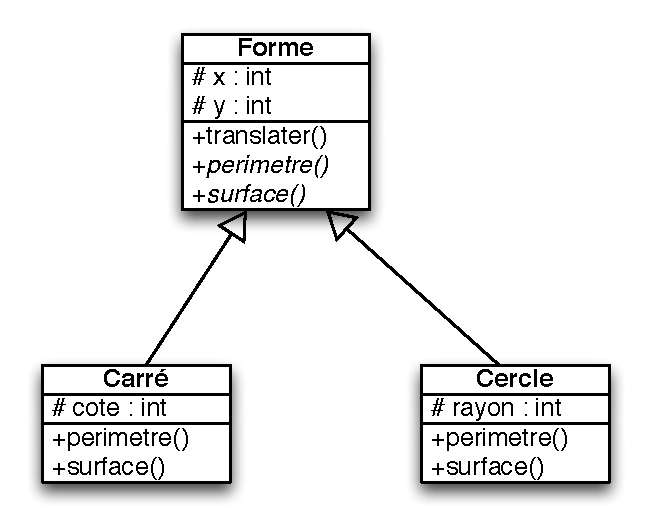
\includegraphics[height=5cm]{fig/forme1.pdf}
\end{center}
\end{frame}


%\section{Généricité}

\section{Les exceptions}
\label{sec:exceptions}

% partie sur les exceptions

\subsection{Introduction}

\begin{frame}{Introduction}
\begin{itemize}
\item Un programme peut contenir des erreurs de syntaxe (voire de grammaire), celles-ci sont détectées par le compilateur, mais aussi des erreurs logiques qui se voient (ou pas) à l'exécution. 
\item De plus, l'utilisateur peut lui aussi commettre des erreurs, i.e. avoir un comportement imprévu
\end{itemize}
\begin{center}
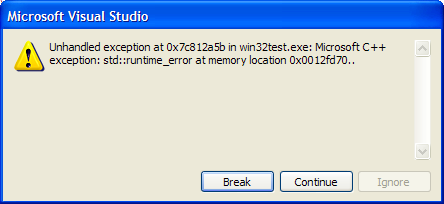
\includegraphics[height=3cm]{fig/exception2.png} 
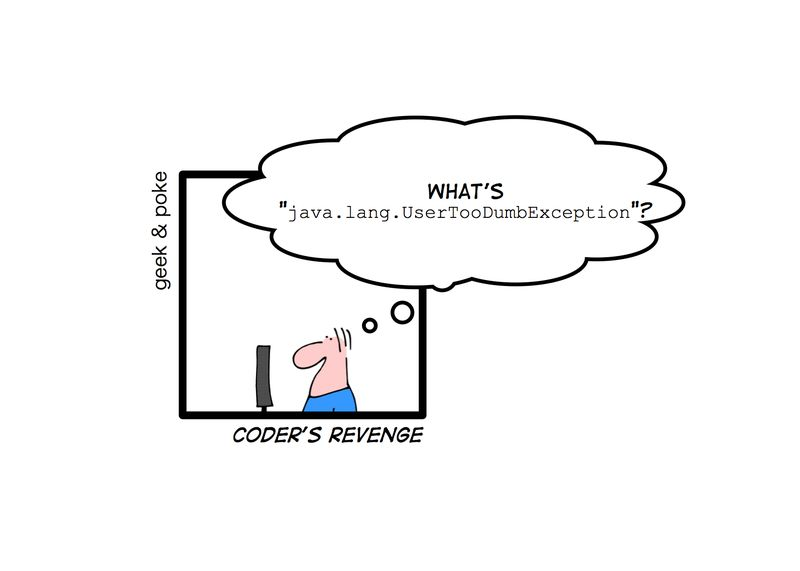
\includegraphics[height=3cm]{fig/usertoodumb.jpg}
\end{center}
\end{frame}

\begin{frame}{Que peut-on faire ?}
\begin{itemize}
\item Erreurs de compilation : facile !
\item Des tests !
\begin{itemize}
\item Voir le cours de MEDEV pour les tests unitaires, tests d'intégration, plans de tests
\item Mais aussi : la preuve de programme ou de propriétés, etc. 
\end{itemize}
\item Vérifier que tout se passe bien pendant l'exécution du programme
\begin{itemize}
\item Vérifier que les actions de l'utilisateur sont valides
\item Vérifier que certaines valeurs de variables sont appropriées (assertions)
\item Ne pas juste planter un programme quand quelque chose ne va pas
\end{itemize}
\item Pour autant, on ne va pas y passer notre vie...
\end{itemize}
\end{frame}

\subsection{Les assertions}

\begin{frame}[fragile]\frametitle{Les assertions : arrêter un programme à temps}
\begin{itemize}
\item \structure{pré-conditions} : on sait que certaines fonctions s'exécutent dans certaines conditions 
\item Sans aller jusqu'à la \href{http://fr.wikipedia.org/wiki/Programmation_par_contrat}{programmation par contrat}, on peut valider certaines pré-conditions importantes
\item C'est l'étape qui suit ... l'écriture des pré-conditions dans la documentation !
\item Mieux vaut les utiliser en mode debug que production
\end{itemize}
\begin{codeblock}{Exemple}
\begin{lstlisting}
#include <cassert>
using namespace std;

bool compte::debiter(float montant) {
    assert((montant >= 0));
    if (!ib && solde>=montant) {
        solde -= montant;
        return true;
    }
    return false;
}
\end{lstlisting}
\end{codeblock}
\end{frame}

\begin{frame}[fragile]\frametitle{Résultat}
\begin{itemize}
%\item Si l'assertion est vérifiée, rien ne se passe
\item Si l'assertion n'est pas vérifiée, message d'erreur et arrêt du programme
\begin{block}{Résultat avec un débit de -1000}
{\tiny 
\begin{verbatim}
Assertion failed: ((montant >= 0)), function debiter, file /Users/moreau/Documents/Enseignement/optionRV/CPLUS/code/compte.cxx, line 26.
Abort
\end{verbatim}}
\end{block}
\item Il vaut mieux utiliser des assertions claires...
\item \alert{Attention} : l'assertion est une technique de détection des erreurs de programmation et non pas de gestion des erreurs d'exécution !
\begin{itemize}
\item En clair, elles sont réservées au développeur 
\item Les assertions ne sont pas vérifiées dans un programme compilé en mode Release
\item Conséquence : éviter les expressions du type \verb|assert(index++ < MAXVAL)|
\item On peut les supprimer en compilant avec \verb|-DNDEBUG|
\end{itemize}
\end{itemize}
\end{frame}


\subsection{Utilisation des exceptions en C++}

\begin{frame}[fragile]
\frametitle{Exemple introductif}
\begin{itemize}
\item C++ ne nous facilite pas énormément la vie par défaut pour la gestion des erreurs 
\end{itemize}
\begin{codeblock}{Exemple}
\begin{lstlisting}
int division(int a, int b) {
    return a/b;
}

int main() {
    int tab[SZ];
    char * a = "lorsque l'enfant parait, son doux regard qui brille...";
    for (int i=0 ; i<=SZ+1 ; i++) {
        tab[i] = i*i;
    }
    
    for (int i=0 ; i<=SZ+1 ; i++) {
        std::cout << "tab[" << i << "] = " << tab[i] << std::endl;
    }
    
    std::cout << a << std::endl;
    
    std::cout << division(24,4) << std::endl;
    std::cout << division(24,0) << std::endl;
    
}
\end{lstlisting}
\end{codeblock}
\end{frame}

\begin{frame}[fragile]
\frametitle{Résultat}
\begin{block}{Exécution (pas forcément répétable)}
{\tiny 
\begin{verbatim}
tab[0] = 0
tab[1] = 1
tab[2] = 4
tab[3] = 9
tab[4] = 16
tab[5] = 25
tab[6] = 36
tab[7] = 49
tab[8] = 64
tab[9] = 81
tab[10] = 100
tab[11] = 121
lorsque l'enfant parait, son doux regard qui brille...
6
Floating exception
\end{verbatim}
}
\end{block}
\begin{itemize}
\item Les dépassements de tableau peuvent avoir une incidence ... ou pas
\item La division par zéro fait planter le programme
\end{itemize}
\end{frame}

\begin{frame}[fragile]
\frametitle{Quelques possibilités pour gérer les erreurs (1/2)}
\begin{itemize}
\item Renvoyer une valeur prédéfinie à la place du résultat
\begin{lstlisting}
#define ERROR_DIV_BY_0 -125

int division(int a, int b) {
    if (b !=0 ) {
        return a/b;
    }
    else {
        return ERROR_DIV_BY_0;
    }
}
\end{lstlisting}
\begin{itemize}
\item il faudrait être sûr que la valeur de \verb|ERROR_DIV_BY_0| n'est pas un résultat possible
\item l'utilisateur de la division va-t-il vraiment s'en soucier ?
\end{itemize}
\item Afficher un message d'erreur
\begin{lstlisting}
        std::cerr << "tentative de division par 0" << std::endl;
\end{lstlisting}
\begin{itemize}
\item message pour l'utilisateur final ? dans un programme avec GUI ?
\item Valeur de retour de la fonction dans ce cas ?
\end{itemize}
\end{itemize}
\end{frame}

\begin{frame}[fragile]
\frametitle{Quelques possibilités pour gérer les erreurs (2/2)}
\begin{itemize}
\item Gestion des erreurs "à la C" : retour de la fonction booléen et passage de la vraie valeur par adresse
\begin{lstlisting}
bool division_faconC(int a,int b,int &r) {
    if (b != 0) {
        r = a/b;
        return true;
    }
    else {
        return false;
    }
}
\end{lstlisting}
\begin{itemize}
\item Lourd mais efficace
\item Franchement pas intuitif
\end{itemize}
\end{itemize}
\end{frame}

\begin{frame}{Principe des exceptions}
\begin{itemize}
\item On va délimiter les zones \textit{à risque} d'un programme, c'est-à-dire les zones où il peut se produire quelque chose d'anormal
\item Si une erreur survient dans ces zones, on \struc{lève une exception} à l'aide d'un objet qui contient des informations sur l'erreur
\item Quelque part dans le code (à l'endroit où c'est le plus approprié), on gère l'erreur en \struc{attrapant l'exception} 
\item Si aucun code n'attrape l'exception, le programme s'arrête
\end{itemize}
\end{frame}

\begin{frame}[fragile]\frametitle{Les exceptions en C++}
\begin{itemize}
\item Les exceptions en C++ font appel à trois mots-clés
\begin{itemize}
\item \verb|try{ ... }| délimite le morceau de code susceptible de lever des exceptions
\item \verb|throw| \textit{expression} permet de lever une exception
\begin{itemize}
\item \verb|throw| doit de préférence se trouver dans un bloc \verb|try { ... }|
\end{itemize}
\item \verb|catch(...) { ... }| permet d'attraper une exception
\begin{itemize}
\item Les blocs \verb|catch(...) { ... }| suivent obligatoirement un bloc \verb|try { ... }|
\item On peut associer plusieurs \verb|catch| à un seul \verb|try|, il en faut au moins un par type d'\textit{expression} lancée par le \verb|throw|
\end{itemize}
\end{itemize}
\end{itemize}
\end{frame}

\begin{frame}[fragile]
\frametitle{Exemple : gestion de la division par zéro (1/2)}
\begin{enumerate}
\item Inclusion d'un bloc \verb|try|
\item Ajout d'un \verb|throw| pour lever une exception
\item Ajout d'un bloc \verb|catch|
\end{enumerate}
\begin{lstlisting}
int division(int a, int b) {
    try {
        if (b !=0 ) {
            return a/b;
        }
        else {
            throw std::string("Division par zero !");
        }
    }
    catch (std::string const& err_msg) {
        std::cerr << "Exception: " << err_msg << std::endl;
    }
}
\end{lstlisting}
\begin{itemize}
\item On est retourné au simple affichage du message d'erreur...
\begin{itemize}
\item Parce qu'on ne gère pas l'erreur à l'endroit approprié
\end{itemize}
\end{itemize}
\end{frame}

\begin{frame}[fragile]
\frametitle{Exemple : gestion de la division par zéro (2/2)}
\begin{itemize}
\item Nouvelle version 
\begin{itemize}
\item Plus de \verb|try| dans la fonction division mais dans son utilisation
\end{itemize}
\begin{lstlisting}
int division(int a, int b) {
        if (b !=0 ) {
            return a/b;
        }
        else {
            throw std::string("Division par zero !");
        }
}
\end{lstlisting}
\item Le code après le \verb|throw| n'est pas exécuté, donc pas de problème de valeur de retour
\item Utilisation
\begin{lstlisting}
    try {
        std::cout << division(24,4) << std::endl;
        std::cout << division(24,0) << std::endl;
    }
    catch(const std::string& err_msg) {
        std::cerr << "Exception : " << err_msg << std::endl;
    }
\end{lstlisting}
\end{itemize}
\end{frame}

\begin{frame}{Plus formellement...}
\begin{itemize}
	\item Une exception est un signal
	\begin{itemize}
		\item qui indique que quelque chose d'exceptionnel (par exemple une erreur) s'est produit
		\item qui interrompt le flot d'exécution normal du programme
	\end{itemize}
	\item lancer (\textbf{\texttt{throw}}) une exception revient à signaler quelque chose
	\item attraper (\textbf{\texttt{catch}}) une exception permet d'exécuter les actions nécessaires au traitement de la situation particulière
\end{itemize}
\end{frame} 


%%%%%%%%%%%%%%%%%%%%%%%%%%%%%%%%%%%%%%%%%%%%%%%%
\begin{frame}{Les exceptions : mécanisme}
\begin{itemize}
	\item lorsqu'une situation exceptionnelle est rencontrée une exception est lancée
	\item si cette exception n'est pas attrapée dans le bloc de code dans lequel elle se trouve, elle est propagée au bloc de code supérieur et ainsi de suite...
	\item même principe pour les fonctions/méthodes...
	\item si une exception n'est jamais attrapée :
	\begin{itemize}
		\item propagation jusqu'au main()
		\item affichage d'un message d'erreur
		\item arrêt de l'exécution du programme
	\end{itemize}
\end{itemize}
\end{frame} 

\begin{frame}{Pourquoi des objets Exception ?}
\begin{itemize}
	\item \alert{Transparent issu du cours de Java !}
	\item La représentation des objets sous forme d'objets permet de mieux structurer la description et le traitement des erreurs
\end{itemize}
{\small \begin{quote}
"Because all exceptions that are thrown within a Java program 
are first-class objects, grouping or categorization of exceptions 
is a natural outcome of the class hierarchy.  Java exceptions 
must be instances of Throwable or anyThrowable descendant. 
As for other Java classes, you can create subclasses of the 
Throwable class and subclasses of yoursubclasses. 
Each "leaf" class (a class with no subclasses) represents 
a specific type of exception and each "node" class (a class with 
one or more subclasses) represents a group of 
related exceptions. "
\end{quote}}
\end{frame} 

\begin{frame}[fragile]\frametitle{Les objets \texttt{exception}}
\begin{itemize}
\item En C++, on peut lancer des exceptions de n'importe quel type
\item Pour mieux comprendre ce qui s'est passé, il serait intéressant d'avoir
\begin{itemize}
\item une description de l'erreur
\item l'endroit où elle se situe (fichier, ligne, pile d'appels)
\item d'éventuelles informations complémentaires selon l'erreur
\end{itemize}
\item La bibliothèque standard de C++ fournit une classe \verb|exception|
\begin{itemize}
\item Utilisation avec \verb|#include <exception>|
\item Les méthodes sont virtuelles, polymorphisme plus que recommandé
\end{itemize}
\item Pourquoi construire des classes dérivées de \verb|exception| ?
\begin{itemize}
\item Gérer ses propres erreurs
\item Hiérarchiser les types d'erreurs
\item Profiter de cette hiérarchie dans les bloc \verb|catch|
\end{itemize}
\end{itemize}
\end{frame}

\begin{frame}[fragile]\frametitle{Quelques classes dérivées d'\texttt{exception} (1/2)}
Exceptions susceptibles d'être levées par la bibliothèque standard
\begin{tabular}{|l|l|}
\hline Classe & Description \\ 
\hline \verb|bad_alloc| & Problème d'allocation mémoire \\ 
\hline \verb|bad_cast| & Erreur lors d'un \verb|dynamic_cast| \\
\hline \verb|bad_exception| & Pas de \verb|catch| correspondant à une exception levée \\
\hline \verb|bad_typeid| & erreur à l'utilisation de \verb|typeid| \\
\hline \verb|ios_base::failure| & problème avec un flot de données \\
\hline
\end{tabular} 
\end{frame}

\begin{frame}[fragile]\frametitle{Quelques classes dérivées d'\texttt{exception} (2/2)}
Quelques types d'exceptions pré-définies (dans \verb|stdexcept|) à réutiliser
\begin{tabular}{|l|l|}
\hline Classe & Description \\ 
\hline \verb|domain_error| & Erreur de domaine (maths) \\
\hline \verb|invalid_argument| & argument invalide (en valeur) passé à une fonction \\
\hline \verb|length_error| & taille invalide \\
\hline \verb|out_of_range| & erreur d'indice de tableau \\
\hline \verb|logic_error| & erreur logique (algo) \\
\hline
\end{tabular}
\begin{itemize}
\item Par exemple, dans l'exemple de la division, on aurait pu lever une \verb|domain_error|
\item \verb|out_of_range| pourrait être utilisé par \verb|vector<?>| pour signaler un indice hors limite
\begin{itemize}
\item En réalité, on aura plutôt un \verb|vector::_M_range_check|
\end{itemize} 
\end{itemize} 
\end{frame}

\section{La bibliothèque standard}

% la STL

\begin{frame}{Introduction}
\label{secstl}
\begin{itemize}
\item \hypertarget{pdf:stl}{Un} langage de programmation a besoin d'une bibliothèque d'interaction avec le système
\begin{itemize}
\item On ne peut pas se contenter de faire tourner des algorithmes en rond sans entrées/sorties
\item Et même pour écrire des algorithmes, on ne veut pas (mal) réinventer la roue à chaque fois
\end{itemize}
\item Les fonctions livrées avec C++ ont longtemps été le parent pauvre du langage (notamment par rapport à Java)
\item Pire, dans les anciennes versions C++ (i.e. avant la normalisation), on trouvait des bibliothèques (très) variables
\item On s'intéresse à la version normalisée C++11 de la \textit{SL}
\begin{itemize}
\item pas de doc officielle d'utilisation, juste une description fonctionnelle dans la norme...
\item Néanmoins, très bonne doc : \url{http://www.cplusplus.com/reference/}
\end{itemize}
\end{itemize}
\end{frame}

\begin{frame}[fragile]\frametitle{Contenu}
\begin{itemize}
\item 3 grandes parties dans la \textit{SL}
\begin{itemize}
\item Un héritage du C (nécessaire)
\item La STL (\textit{Standard Template Library}) et les flots
\item Le reste (dont les \verb|string|, les \verb|namespace|)...
\end{itemize}
\end{itemize}
\end{frame}

\subsection{L'héritage du C}

\begin{frame}[fragile]\frametitle{L'héritage du C}
\begin{itemize}
\item En C, on avait pris l'habitude de faire des \verb|#include <math.h>|
\item En C++, on les remplace progressivement par \verb|#include <cmath>|
\item On y ajoute parfois un \verb|using namespace std;|
\begin{itemize}
\item permet d'écrire \verb|sqrt(2)| au lieu de \verb|std::sqrt(2.0)|
\end{itemize}
\item Tout ce qui était utilisé en C est encore disponible sous cette nouvelle dénomination, mais pas forcément utile
\end{itemize}
\end{frame}

\subsection{La STL}

\begin{frame}{La STL}
\begin{itemize}
\item STL : Standard Template Library
\item On parle aussi de bibliothèques de conteneurs (parce les structures fournies ne sont seront pas liées à un type donné)
\item Correspond au \textit{Collection Framework} de java
\begin{itemize}
\item en beaucoup plus puissant
\item et peut s'avérer beaucoup plus compliqué également...
\end{itemize}
\item Commençons par un exemple : le vecteur
\begin{itemize}
\item Alternative pratique aux tableaux standards du C
\end{itemize}
\end{itemize}
\end{frame}

\begin{frame}[fragile]\frametitle{Le conteneur \texttt{vector}}
\begin{itemize}
\item Les listes sont une des abstractions les plus utiles en programmation
\begin{itemize}
\item Que faire avec ? créer, parcourir, rechercher, ajouter, supprimer...
\end{itemize}
\item Toujours les mêmes algorithmes quel que soit le type d'éléments de la liste
\item Structure et algorithmes universels : réutiliser ce qui a déjà été (bien) écrit (et testé)
\item C++ fournit la structure \verb|vector<type>| où \verb|type| est à remplacer par un type de données
\begin{itemize}
\item  \verb|vector<int>| pour un vecteur d'entiers
\item \verb|vector<forme>| pour un vecteur de formes
\item \verb|vector<forme*>| pour un vecteur de pointeurs sur des formes
\item \verb|vector<vector<float> >| pour une vecteur de vecteurs de réels
\end{itemize}
\end{itemize}
\end{frame}

\begin{frame}[fragile]\frametitle{Exemple d'utilisation de \texttt{vector}}
\begin{lstlisting}
#include <vector>
#include <iostream>
using namespace std;

int main() {
    vector<int> v1;
    v1.push_back(5);
    v1.push_back(8);
    for (int i(0) ; i<8 ; i++) {
        v1.push_back(i);
    }
    cout << "taille : " << v1.size() << endl;

    for (int i(0) ; i<v1.size() ; i++) {
        cout << v1[i] << endl;
    }

    // syntaxe alternative
    for (int& x : v1) {
        cout << x << endl;

    }
}
\end{lstlisting}
\end{frame}

\begin{frame}[fragile]\frametitle{Conteneurs pour les structures linéaires}
\begin{itemize}
\item Rappel : suivant la structure interne utilisée (liste chaînée ou tableau par exemple), une structure linéaire est plus ou moins efficace selon les opérations
\item C++ met à disposition 2 grands types de structures linéaires qui s'utilisent en grande partie de façon identique
\begin{itemize}
\item Les séquences
\begin{itemize}
\item \verb|vector| \urldoc{http://www.cplusplus.com/reference/vector/vector/} : tableau classique
\item \verb|deque| \urldoc{http://www.cplusplus.com/reference/deque/deque/} : liste doublement chaînée (\textit{double ended queue})
\item \verb|list| \urldoc{http://www.cplusplus.com/reference/list/list/} : conteneur générique pour l'utilisation des itérateurs
\item \verb|stack| \urldoc{http://www.cplusplus.com/reference/stack/} : pile
\item \verb|queue| \urldoc{http://www.cplusplus.com/reference/queue/} : file (structure FIFO)
\item \verb|priority_queue| \urldoc{http://www.cplusplus.com/reference/queue/priority_queue/} : file avec priorité (suppose des éléments comparables)
\end{itemize}
\item Les tableaux associatifs
\begin{itemize}
\item \texttt{set} \urldoc{http://www.cplusplus.com/reference/set/set/}
\item \texttt{multiset} \urldoc{http://www.cplusplus.com/reference/set/multiset/}
\item \texttt{map} \urldoc{http://www.cplusplus.com/reference/map/map/}
\item \texttt{multimap} \urldoc{http://www.cplusplus.com/reference/map/multimap/}
\end{itemize}
\end{itemize}
\end{itemize}
\end{frame}

\begin{frame}[fragile]\frametitle{Utilisation la plus commune possible}
\begin{itemize}
\item C++ essaie au maximum de faciliter l'utilisation des conteneurs
\begin{itemize}
\item inclusion : \verb|#include <conteneur>|
\item quelques méthodes communes
\begin{itemize}
\item \verb|empty()|
\item \verb|size()|
\item \verb|clear()|
\end{itemize}
\item Utilisation maximale de la surcharge des opérateurs (vu pour l'accès à des éléments d'un vecteur)
\end{itemize}
\end{itemize}
\end{frame}

\subsubsection{Les séquences}

\begin{frame}[fragile]\frametitle{Retour sur les vecteurs}
\begin{itemize}
\item Documentation : \url{http://www.cplusplus.com/reference/vector/vector/}
\item Accès aux éléments
\begin{itemize}
\item \verb|operator[]()| pour les accès type tableau
\item \verb|push_back()| pour ajouter à la fin
\item \verb|pop_back()| pour récupérer le dernier élément et l'enlever
\item \verb|front()| premier élément
\item \verb|back()| dernier élément
\end{itemize}
\item En réalité, ces méthodes sont communes à toutes les classes de séquence
\end{itemize}
\end{frame}

\subsubsection{Les tableaux associatifs}

\begin{frame}{Les tableaux associatifs}
\begin{itemize}
\item Dans un \texttt{vector}, les éléments sont accessibles via l'opérateur \texttt{[]} et leur indice qui est un nombre entier
\item On n'a pas toujours besoin d'un indice entier (exemple : dictionnaire)
\item Les tableaux associatifs généralisent la notion de tableau en permettant l'utilisation de n'importe quel type comme indice
\begin{itemize}
\item Déclaration : \texttt{map<}\textit{clé}\texttt{,}\textit{valeur}\texttt{>} \urldoc{http://www.cplusplus.com/reference/map/map/}
\item Le type de clé doit être ordonné
\end{itemize}
\item On parle d'association (\textit{map} en anglais) car à une clé  est associée une valeur \textbf{unique}
\item C'est une notion très courante dans les langages du web comme PhP
\item Les méthodes d'accès sont en ${\cal O}(\log n)$
\end{itemize}
\end{frame}

\begin{frame}[fragile]\frametitle{Utilisation des \texttt{map}}
\begin{itemize}
\item \verb|m.count(key)| : renvoie 1 si la clé est présente, 0 sinon
\item \verb|m.find(key)| : renvoie un itérateur vers la clé ou \verb|m.end()| sinon
\item \verb|m.at(key)| : renvoie la valeur associée  ou exception \verb|out_of_range|
\item \verb|m[key]| : renvoie la valeur associée ou une référence vers une nouvelle valeur
\end{itemize}
\begin{codeblock}{Exemple d'utilisation}
\begin{lstlisting}
    map<string,string> dict;
    dict["banane"] = "banana";
    dict["poire"] = "pear" ;
    dict["pomme"] = "apple";
    cout << (dict.count("cerise")>0 ? "trouve" : "pas trouve") << endl;
    cout << dict.size() << endl;
    cout << dict["framboise"] << endl;
    cout << dict.size() << endl;
\end{lstlisting}
\end{codeblock}
\begin{exampleblock}{Résultat}
{\tiny
\begin{verbatim}
pas trouve
3

4
\end{verbatim}
}
\end{exampleblock}
\end{frame}

\begin{frame}[fragile]\frametitle{Autres conteneurs associatifs}
\begin{itemize}
\item Ils s'utilisent de la même manière
\item Quelques propriétés particulières de chaque type
\begin{itemize}
\item Les \verb|set| \urldoc{http://www.cplusplus.com/reference/set/set/} sont utilisés pour représenter les ensembles, au sens mathématique (insertion et recherche, pas d'accès via []). Fusion valeur/clé en quelque sorte
\item Les \verb|multiset| \urldoc{http://www.cplusplus.com/reference/set/multiset/} sont des ensembles où une valeur peut apparaître plusieurs fois
\item Les \verb|multimap| \urldoc{http://www.cplusplus.com/reference/map/multimap/} sont des \verb|map| où une même clé peut apparaître plusieurs fois
\end{itemize}
\end{itemize}
\end{frame}

\subsubsection{Les itérateurs}

\begin{frame}[fragile]\frametitle{Les itérateurs}
\begin{itemize}
\item Souvenirs de C : le parcours d'une liste se fait en
\begin{itemize}
\item incrémentant un indice $i$ dans le cas d'un tableau
\item en faisant avancer un \textit{pointeur courant} dans le cas d'une liste chaînée
\begin{lstlisting}
ptr = ptr->next;
\end{lstlisting}
\end{itemize}
\item En première approximation, les itérateurs peuvent être vus comme des pointeurs sur les éléments des conteneurs
\item En réalité, ce sont des objets complexes !
\item Analogie avec le pointeur
\begin{itemize}
\item on le fait avancer avec \texttt{++} et reculer avec \texttt{--}
\item on accède à l'élément via l'opérateur de déréférencement \texttt{*}
\end{itemize}
\end{itemize}
\end{frame}

\begin{frame}[fragile]\frametitle{Utilisation}
\begin{itemize}
\item Déclaration : \textit{conteneur}\texttt{::iterator} \textit{nom}\texttt{;}
\begin{lstlisting}
vector<int> tab(5,5);
vector<int>::iterator it;
\end{lstlisting}
\item Itération et utilisation
\begin{lstlisting}
int total = 0;
for (it=tab.begin() ; it!=tab.end() ; it++) {
  total += *it;
}
\end{lstlisting}
\item où \verb|tab.begin()| renvoie un itérateur sur le début de la liste et \verb|tab.end()| un itérateur sur l'élément (invalide) qui suit juste le dernier élément
\item Sur certains types de conteneurs (\verb|vector| et \verb|deque|), l'arithmétique de pointeurs est autorisée (\textit{random access iterators})
\begin{lstlisting}
    *(tab.begin()+3) = 2; // modification du 4eme element
    cout << tab[3] << endl;
\end{lstlisting}
\end{itemize}
\end{frame}

\begin{frame}[fragile]\frametitle{Itérateurs et \texttt{list}}
\begin{itemize}
\item Les \verb|list| sont des structures de listes chaînées dont les éléments sont non contigus en mémoire
\item Les itérateurs constituent le seul moyen d'accès au contenu
\begin{lstlisting}
    list<string> todo;
    todo.push_back("repeindre la cuisine");
    todo.push_back("finir le poly de C++");
    todo.push_back("dormir");

    for (list<string>::iterator i=todo.begin() ; i!=todo.end() ; ++i) {
        cout << "TODO: " << *i << endl;
    }
\end{lstlisting}
\item Syntaxe alternative (et réductrice)
\begin{lstlisting}
    for (string& s : todo) {
        cout << "TODO: " << s << endl;

    }
\end{lstlisting}
\end{itemize}
\end{frame}

\begin{frame}[fragile]\frametitle{Itérateurs et \texttt{map}}
\begin{itemize}
\item C'est un peu plus compliqué puisque les \verb|map| sont des paires $(key,value)$
\item Ca se traduit en C++ par une classe \verb|pair<T,E>| (déclarées dans \verb|utility|) à deux attributs appelés \verb|first| et \verb|second|
\item les itérateurs des \verb|map<T,E>| se déréférencent vers des \verb|pair<K,E>|
\end{itemize}
\begin{codeblock}{Utilisation}
\begin{lstlisting}
    for(map<string,string>::iterator itmap=dict.begin() ; itmap!=dict.end() ; ++itmap) {
        cout << "dict[" << itmap->first << "] = " << itmap->second << endl;
    }
\end{lstlisting}
\end{codeblock}
\begin{block}{Résultat}
{\tiny
\begin{verbatim}
dict[banane] = banana
dict[framboise] =
dict[poire] = pear
dict[pomme] = apple
\end{verbatim}
}
\end{block}
\end{frame}

% foncteurs et algorithmes

\subsection{Foncteurs}

\begin{frame}{Foncteurs}

\begin{itemize}
\itemsep1pt\parskip0pt\parsep0pt
\item
  On aimerait pouvoir appliquer des algorithmes à des collections (au
  sens de la STL)

  \begin{itemize}
  \itemsep1pt\parskip0pt\parsep0pt
  \item
    on peut le faire en créant une fonction qui prend une collection en
    paramètre
  \item
    l'inverse pourrait être pratique : passer la fonction elle-même
    comme paramètre
  \end{itemize}
\item
  C'est le principe des \structure{foncteurs}

  \begin{itemize}
  \itemsep1pt\parskip0pt\parsep0pt
  \item
    On peut aussi utiliser aussi les pointeurs de fonction
  \item
    Un foncteur est une classe qui surcharge l'opérateur \texttt{()} qui effectue
    l'opération souhaitée
  \end{itemize}
  \item Note hors sujet : c'est le principe des \textit{shaders}...
\end{itemize}

\end{frame}

\begin{frame}[fragile]\frametitle{Exemple simpliste}
\begin{itemize}
\item Création du foncteur
\begin{codeblock}{Classe addition}
\begin{lstlisting}
class addition{
public:
    int operator()(int a, int b) {
        return a+b;
    }
};
\end{lstlisting}
\end{codeblock}
\begin{codeblock}{Utilisation}
\begin{lstlisting}
    addition foncteur;
    cout << "2+4 = " << foncteur(2,4) << endl;
\end{lstlisting}
\end{codeblock}
\begin{block}{Résultat}
{\tiny
\begin{verbatim}
2+4 = 6
\end{verbatim}}
\end{block}
\end{itemize}
\end{frame}

\begin{frame}[fragile]\frametitle{Exemple : valeur absolue}
\begin{itemize}
\item Création du foncteur
\begin{codeblock}{Classe addition}
\begin{lstlisting}
class valeurabsolue {
public:
    int operator()(int a) {
        if (a>=0) {
            return a;
        }
        else {
            return -a;
        }
    }
};
\end{lstlisting}
\end{codeblock}
\item On verra par la suite comment l'appliquer à une collection
\end{itemize}
\end{frame}

\begin{frame}[fragile]\frametitle{Plus complexe : remplir une collection avec des valeurs différentes}
\begin{itemize}
\item Les foncteurs sont des objets, ils peuvent avoir des attributs
\item Exemple : un foncteur renvoie une valeur incrémentée à chaque appel
\end{itemize}
\begin{codeblock}{Classe fill}
\begin{lstlisting}
class myfill {
private:
    int m;
public:
    myfill(int i) : m(i) {}
    int operator()() {
        ++m;
        return m;
    }
};
\end{lstlisting}
\end{codeblock}
\begin{codeblock}{Utilisation}
\begin{lstlisting}
    myfill f(22);
    for (vector<int>::iterator i=v1.begin() ; i!=v1.end() ; ++i) {
        *i = f();
    }
\end{lstlisting}
\end{codeblock}
\end{frame}

\begin{frame}{Les prédicats}

\begin{itemize}
\itemsep1pt\parskip0pt\parsep0pt
\item
  les prédicats sont des expressions booléennes (vient de la logique)
\item
  En C++, ce sont des foncteurs particuliers renvoyant un booléen
\item
  Ils sont utilisés pour tester une valeur particulière d'un objet

  \begin{itemize}
  \itemsep1pt\parskip0pt\parsep0pt
  \item
    nombre plus grand que 10
  \item
    cette chaîne contient-elle des voyelles ?
  \item
    Cet objet est-il encore valide ?
  \end{itemize}
\item
  Ils seront très utiles dans les algorithmes de la STL
\end{itemize}

\end{frame}

\begin{frame}[fragile]\frametitle{Les foncteurs prédéfinis}

\begin{itemize}
\itemsep1pt\parskip0pt\parsep0pt
\item
  La STL fournit un certain nombre de foncteurs
\item
  Ils sont déclarés dans \verb|functional| \urldoc{http://www.cplusplus.com/reference/functional/}
  \item Ils sont paramétrés par un type (i.e. on peut choisir le type auquel ils s'appliquent)
\item
  On y trouve notamment

  \begin{itemize}
  \itemsep1pt\parskip0pt\parsep0pt
  \item
    les opérateurs arithmétiques (\verb|plus<T>|)
  \item
    les opérateurs de comparaison (\verb|equal_to<T>|)
  \item
    les opérateurs logiques (\verb|logical_and<T>|)
  \item
    des adaptateurs et des convertisseurs
  \item
    d'autres choses encore...
  \end{itemize}
\end{itemize}

\end{frame}

\subsection{Les algorithmes : lier conteneurs et foncteurs}

\begin{frame}[fragile]\frametitle{Les algorithmes : lien entre conteneurs et foncteurs}

\begin{itemize}
\itemsep1pt\parskip0pt\parsep0pt
\item
  Par algorithme, on entend les fonctions définies dans \verb|algorithm| \urldoc{http://www.cplusplus.com/reference/algorithm/}
\item
  Ce sont des fonctions génériques qui prennent en argument des
  conteneurs (ou du moins des itérateurs) et des foncteurs

  \begin{itemize}
  \itemsep1pt\parskip0pt\parsep0pt
  \item
    elles appliquent les foncteurs à chaque élément du conteneur (entre
    les itérateurs de début et de fin)
  \end{itemize}
\item
  Objectif : profiter à la fois de la puissance de la STL et de la
  qualité des algorithmes fournis (exemple : tri)
\item Pas moins de 85 algorithmes sont proposés par la STL (et ce sont tous des \textit{templates})
\item Les algorithmes s'appliquent à tous les conteneurs
\begin{itemize}
\item Aux restrictions sur les types d'itérateurs près
\end{itemize}
\end{itemize}
\end{frame}

\begin{frame}[fragile]\frametitle{Remplissage d'un vecteur}
\begin{itemize}
\item Rappel : nous avons conçu un foncteur \verb|myfill|
\item Son application donnait lieu à une boucle, limitant son intérêt
\begin{codeblock}{Version sans algorithme}
\begin{lstlisting}
    myfill f(22);
    for (vector<int>::iterator i=v1.begin() ; i!=v1.end() ; ++i) {
        *i = f();
    }
\end{lstlisting}
\end{codeblock}
\item Nouvelle version avec l'utilisation de l'algorithme \verb|generate|
\begin{codeblock}{Version avec algorithme}
\begin{lstlisting}
    myfill f1(22);
    generate(v1.begin(),v1.end(),f1);
\end{lstlisting}
\end{codeblock}
\item Utilisation des itérateurs obligatoire (plus puissant)
\begin{itemize}
\item \textbf{Tous les algorithmes utiliseront des itérateurs plutôt que des conteneurs}
\end{itemize}
\end{itemize}
\end{frame}

\begin{frame}[fragile]\frametitle{Remplissage aléatoire et comptage}
\begin{itemize}
\item On veut écrire un code qui remplit un vecteur de façon aléatoire et qui compte le nombre de fois où apparait un nombre donné
%\item Foncteur de remplissage aléatoire
\pause\begin{codeblock}{classe \texttt{randomfill}}
\begin{lstlisting}
class randomfill {
private:
    int max;
public:
    randomfill(int m) : max(m) {}
    int operator()() {
        return rand()%max;
    }
};
\end{lstlisting}
\end{codeblock}
%\item Utilisation des algorithmes \verb|generate| et \verb|count|
\pause\begin{codeblock}{Code d'utilisation}
\begin{lstlisting}
    vector<int> v2(100);
    randomfill rf(15);
    generate(v2.begin(),v2.end(),rf);
    cout << "v2 contient " << count(v2.begin(),v2.end(),2) << " fois le nombre 2" << endl;
\end{lstlisting}
\end{codeblock}
%\begin{block}{Résultat}
%{\tiny
%\begin{verbatim}
%v2 contient 6 fois le nombre 2
%\end{verbatim}
%}
%\end{block}
\end{itemize}
\end{frame}

\begin{frame}[fragile]\frametitle{Utilisation des prédicats}
\begin{itemize}
\item Écrire un foncteur qui vérifie si une chaîne de caractère contient une voyelle. Compter combien de chaines d'un conteneur contiennent une voyelle avec  \verb|count_if| \urldoc{http://www.cplusplus.com/reference/algorithm/count_if/}
\end{itemize}
\pause\begin{codeblock}{Foncteur pour vérifier si un caractère est une voyelle}
\begin{lstlisting}
class isvowel {
public:
    bool operator()(char c) {
        if (c == 'a' || c == 'e' || c == 'y' || c == 'u' || c == 'i' || c == 'o') {
            return true; }
        else { return false; }
    }
};
\end{lstlisting}
\end{codeblock}
\pause\begin{codeblock}{Foncteur pour vérifier si une chaine contient une voyelle}
\begin{lstlisting}
class containsvowel {
public:
    bool operator()(string const &s) {
        return any_of(s.begin(), s.end(), isvowel());
    }
};
\end{lstlisting}
\end{codeblock}

\end{frame}

\begin{frame}[fragile]\frametitle{Utilisation des prédicats}
\begin{codeblock}{Test du foncteur \texttt{containsvowel}}
\begin{lstlisting}
    containsvowel cv;
    cout << (cv("ghjg") ? "voyelle" : "pas de voyelle") << endl;
    cout << (cv("fe(rgfgt") ? "voyelle" : "pas de voyelle") << endl;
\end{lstlisting}
\end{codeblock}
\pause
\begin{block}{Résultat}
{\tiny
\begin{verbatim}
pas de voyelle
voyelle
\end{verbatim}}
\end{block}
\pause\begin{codeblock}{Application à un conteneur}
\begin{lstlisting}
    list<string> ls;
    ls.push_back("kfkgike");
    ls.push_back("jfjgg");
    ls.push_back("i");
    ls.push_back("ayrud");
    cout << "nb chaine avec voyelle : " << count_if(ls.begin(),ls.end(),cv);
\end{lstlisting}
\end{codeblock}
\pause
\begin{block}{Résultat}
{\tiny
\begin{verbatim}
3
\end{verbatim}}
\end{block}
\end{frame}

\begin{frame}[fragile]\frametitle{Autres algorithmes d'utilisation courante (1/2)}
\begin{itemize}
\item Au delà des opérations déjà contenues dans les conteneurs, on trouve des prédicats pour les opérations courantes
\item Recherche
\begin{itemize}
\item \texttt{find} \urldoc{http://www.cplusplus.com/reference/algorithm/find/} pour faire une recherche (s'utilise comme \texttt{count}))
\item \verb|find_if| \urldoc{http://www.cplusplus.com/reference/algorithm/find_if/} qui permet d'utiliser un foncteur qui précise ce qu'on cherche
\end{itemize}
\item Minimum et maximum
\begin{itemize}
\item \verb|min_element| \urldoc{http://www.cplusplus.com/reference/algorithm/min_element/} permet de trouver le minimum d'un conteneur
\end{itemize}
\item Tri
\begin{itemize}
\item \verb|sort| \urldoc{http://www.cplusplus.com/reference/algorithm/sort/} pour un tri sur des conteneurs avec \textit{random access iterators}, utilise l'opérateur \verb|<| ou un comparateur dédié si utilisé avec 3 arguments
\item \verb|stable_sort| \urldoc{http://www.cplusplus.com/reference/algorithm/stable_sort/} pour un tri stable
\item \verb|is_sorted| \urldoc{http://www.cplusplus.com/reference/algorithm/is_sorted/} qui vérifie si un conteneur est trié
\end{itemize}
\end{itemize}
\end{frame}

% il faudrait mentionner les merger et le foreach
\begin{frame}[fragile]\frametitle{Autres algorithmes d'utilisation courante (2/2)}
\begin{itemize}
\item Application d'une fonction à un conteneur : \verb|for_each| \urldoc{http://www.cplusplus.com/reference/algorithm/for_each/}
\begin{itemize}
\item \verb|for_each| a l'avantage de s'utiliser avec un foncteur ou une simple fonction
\end{itemize}
\item \verb|transform| \urldoc{http://www.cplusplus.com/reference/algorithm/transform/} qui permet de travailler sur deux conteneurs à la fois (par exemple pour additionner des vecteurs terme à terme)
\begin{codeblock}{Exemple}
\begin{lstlisting}
    vector<int> a(50),b(50),c(50);
    generate(a.begin(), a.end(), randomfill(10));
    generate(b.begin(),b.end(), randomfill(10));
    transform(a.begin(),a.end(),b.begin(),c.begin(),plus<int>());
\end{lstlisting}
\end{codeblock}
\begin{itemize}
\item Remarque : on peut utiliser des objets sans les nommer : \verb|plus<int>()|
\end{itemize}
\end{itemize}
\end{frame}

\subsection{Les flux}

\begin{frame}{Introduction}
\begin{itemize}
\item Les flux (flots) sont utilisés par C++ pour les entrées/sorties, que ce soit sous forme de fichier, d'accès réseau ou d'interaction avec l'utilisateur (écran, clavier)
\item Depuis la première année, on manipule un outil bizarre : \texttt{cout} (et \texttt{cin})
\item Rien à voir (à première vue) : il existe différences catégories d'itérateurs (accès aléatoires, bidirectionnels...)
\item Un flux (flot de données) est une séquence sur laquelle on ne peut qu'avancer (i.e. sur laquelle un itérateur sera unidirectionnel)
\item De plus, il y aura certaines restrictions en lecture/écriture sur les itérateurs de flux
\end{itemize}
\end{frame}

\begin{frame}[fragile]{\texttt{cout} et itérateurs}
\begin{codeblock}{Etudions ce morceau de code}
\begin{lstlisting}
#include <iostream>
#include <iterator>
using namespace std;

int main() {
    ostream_iterator<double> it(cout);
    *it = 22.5;
    *it = 2.454;

}
\end{lstlisting}
\end{codeblock}
\begin{block}{Résultat}
{\tiny
\begin{verbatim}
22.52.454[mac-infmat05:optionRV/CPLUS/code] moreau%
\end{verbatim}
}
\end{block}
\begin{itemize}
\item des \texttt{include} sans surprise
\item notation curieuse pour les itérateurs (sans \verb|::|)
\item présence du type paramétrique \textit{a posteriori}
\end{itemize}
\end{frame}

\begin{frame}[fragile]{\texttt{cout} et itérateurs}
\begin{itemize}
\item Il manque un espace. Le 2ème argument précise le délimiteur
\begin{lstlisting}
    ostream_iterator<double> it(cout," ");
\end{lstlisting}
\item Si on utilise \verb|ofstream| au lieu de \verb|ostream|, on peut écrire dans un fichier
\item Plus intéressant, la lecture dans un fichier se fait avec \verb|ifstream|
\begin{itemize}
\item NB : on pourrait se passer des itérateurs (pour l'instant)
\end{itemize}
\begin{codeblock}{Lecture dans un fichier}
\begin{lstlisting}
    ifstream inf("data.txt");
    istream_iterator<double> itf(inf);
    istream_iterator<double> the_end;

    int cpt = 0;
    while (itf != the_end) {
        cout << "valeur numero " << cpt << " : " << *itf << endl;
        *itf++; cpt++;
    }
\end{lstlisting}
\end{codeblock}
\end{itemize}
\end{frame}

\begin{frame}[fragile]\frametitle{Le retour des algorithmes}
\begin{itemize}
\item Cas d'utilisation typique : lecture d'un fichier de valeurs réelles sur lequel on va effectuer des traitements statistiques
\item Utilisation de l'algorithme \verb|copy|
\begin{codeblock}{Lecture d'un vecteur sans boucle}
\begin{lstlisting}
    vector<double> v(10);
    ifstream inf2("data.txt");
    istream_iterator<double> itf2(inf2);
    copy(itf2,the_end,v.begin());
    copy(v.begin(),v.end(),ostream_iterator<double>(cout,"--"));
\end{lstlisting}
\end{codeblock}
\pause\begin{block}{Résultat}
{\tiny
\begin{verbatim}
12.4--24.45--23.455--33.22--45.556--0--0--0--0--0--
\end{verbatim}
}
\end{block}
\pause
\item Problème : le vecteur est pré-dimensionné
\item Solution : remplacer l'itérateur par un \verb|back_insert_iterator<vector<double> >|
\end{itemize}
\end{frame}

\begin{frame}[fragile]\frametitle{Flux et algorithmes}
\begin{codeblock}{Nouvelle version}
\begin{lstlisting}
    vector<double> v;
    ifstream inf2("data.txt");
    istream_iterator<double> itf2(inf2);
    back_insert_iterator<vector<double> > it2(v);
    copy(itf2,the_end,it2);
    copy(v.begin(),v.end(),ostream_iterator<double>(cout,"--"));
\end{lstlisting}
\end{codeblock}
\pause\begin{block}{Résultat}
{\tiny
\begin{verbatim}
12.4--24.45--23.455--33.22--45.556--
12.4--23.455--24.45--33.22--45.556--
\end{verbatim}
}
\end{block}
\begin{itemize}
\item On peut utiliser le mécanisme des algorithmes sur les itérateurs de flux \textbf{sans} charger tout un fichier en mémoire
\item Exercice : donner le max d'un fichier de réels en \textbf{deux} lignes de code !
\end{itemize}
\begin{codeblock}{Réponse}
\begin{lstlisting}
    ifstream if3("data.txt");
    cout << *max_element(istream_iterator<double>(if3),the_end) << endl;
\end{lstlisting}
\end{codeblock}
\end{frame}

\subsection{Cas particulier : flux et chaines de caractères}

\begin{frame}[fragile]
\frametitle{Flux et itérateurs de chaines de caractères}
\begin{itemize}
\item Jusque là, on s'est contenté de \verb|[]| et de \verb|+| pour manipuler les chaines
\item Flux chaines de caractères : \verb|ostringstream| et \verb|istringstream|
\begin{itemize}
\item On récupère la chaine construite avec la méthode \verb|str()|
\end{itemize}
\begin{codeblock}{Exemple}
\begin{lstlisting}
    ostringstream fl;
    fl << "une chaine " << 3.14 ;
\end{lstlisting}
\end{codeblock}
\item Les chaines contiennent également des itérateurs
%\begin{codeblock}{Foncteur de mise en majuscule}
%\begin{lstlisting}
%class toupperfct {
%public:
%    char operator()(char c) const {
%        return toupper(c);
%    }
%};
%\end{lstlisting}
%\end{codeblock}
\begin{codeblock}{Mise en majuscules d'une chaine de caractères}
\begin{lstlisting}
class toupperfct {
public:
    char operator()(char c) const {
        return toupper(c);
    }
};
int main() {
    string ch("Ceci est une chaine");
    transform(ch.begin(), ch.end(), ch.begin(), toupperfct());
    cout << ch << endl;
}
\end{lstlisting}
\end{codeblock}
\end{itemize}
\end{frame}


\section{C++ avancé}

% tout ce qui sort un peu du cadre

% tout ce qui concerne les templates

\subsection{Les templates}

\begin{frame}[t]{Les templates : motivation}
  \begin{itemize}
    \item Rappel : l'ordinateur est là pour simplifier les tâches répétitives
    \begin{itemize}
      \item Cela inclut la programmation elle-même !
    \end{itemize}
    \item Source d'inspiration : la classe \texttt{vector<?>}
    \begin{itemize}
      \item Elle fonctionne sur tout type de données
      \item Elle contient des \emph{vrais} types, pas des \texttt{void *}
      \item Limite les risques d'erreur de manipulation des vecteurs
    \end{itemize}
    \item On a croisé ces \texttt{<?>} un peu partout dans la bibliothèque standard
  \end{itemize}
\end{frame}
%--- Next Frame ---%


\begin{frame}[fragile]\frametitle{Un premier exemple simple}
  \begin{itemize}
    \item On a une fonction classique qui calcule le max de deux entiers
    \end{itemize}
\begin{lstlisting}
  int maximum(int a, int b) {
  if (a>b) {
    return a;
  }
  else {
    return b;
  }
}
  \end{lstlisting}
  \begin{itemize}
\item On aimerait pouvoir l'appliquer à tout type de données, sans avoir à réécrire la fonction
\item A supposer qu'on dispose d'un opérateur \texttt{<} sur le type en question
  \end{itemize}
\end{frame}

%--- Next Frame ---%

\begin{frame}[fragile]\frametitle{Fonctions template}
  \begin{itemize}
    \item Pour créer ces fonctions génériques, on va considérer qu'elles travaillent sur un type abstrait
    \item type abstrait ici = type pas défini au moment où on écrit le code de la fonction
    \item On l'appelle souvent \texttt{T}
    \item On préfixe alors la déclaration de fonction par \texttt{template <typename T>}
    \item On utilise T comme type générique dans la fonction
  \end{itemize}
  \begin{lstlisting}
    template<typename T> T maximumTemplate(const T& a,const T& b) {
      if (a>b) {
        return a;
      }
      else {
        return b;
      }
    }

  \end{lstlisting}
\end{frame}
% %--- Next Frame ---%


\begin{frame}[fragile]\frametitle{Remarques sur l'utilisation}
  \begin{itemize}
    \item Il est recommandé de spécifier le type sur lequel on veut instancier la fonction
    \begin{lstlisting}
      cout << maximumTemplate<double>(2.4,6.5) << endl;
      cout << maximumTemplate<int>(2,4) << endl;
    \end{lstlisting}
    \item Mais ce n'est pas obligatoire
    \begin{lstlisting}
      cout << maximumTemplate(2.4,6.5) << endl;
    \end{lstlisting}
      \item Attention aux ambiguités
      \begin{lstlisting}
        cout << maximumTemplate(2.4,6) << endl;
      \end{lstlisting}
  \end{itemize}
  {\tiny \begin{verbatim}
    maximum.cpp:30:34: warning: implicit conversion from 'double' to 'int' changes value from 2.5 to 2
      [-Wliteral-conversion]
    cout << maximumTemplate<int>(2.5,4) << endl;
            ~~~~~~~~~~~~~~~      ^~~
  \end{verbatim}}
\end{frame}
%--- Next Frame ---%

\begin{frame}[fragile]\frametitle{Précautions d'usage}
  \begin{itemize}
    \item L'utilisation des templates est encore difficile avec certains compilateurs
    \item Conséquences
    \begin{itemize}
      \item Dans la plupart des cas, il faut tout caser dans les .h
      \item Les messages d'erreurs des compilateurs peuvent être complexes à comprendre
    \end{itemize}
    \item Exemple : si vous utilisez un opérateur surchargé (ne serait-ce que \texttt{=}), tous les types \texttt{T} avec lesquels vous emploierez la fonction devront surcharger \texttt{=}
    \begin{itemize}
      \item constructeur par recopie indispensable
    \end{itemize}
    \item Rien ne garantit comment sera utilisée votre fonction template
    \begin{lstlisting}
      maximumTemplate(string("titi"),string("toto")
      maximumTemplate<Elephant>(...,...)
    \end{lstlisting}
  \end{itemize}
\end{frame}
%--- Next Frame ---%

\begin{frame}[fragile]{De la généricité ... mais pas trop !}
  \begin{itemize}
    \item On peut spécialiser les fonctions template (comportement particulier pour une classe spécifique) !
    \item Il suffit de préciser le type sur lequel elle s'applique
    \begin{lstlisting}
      template<> Elephant maximumTemplate(const Elephant&a,const Elephant&b) {
          if (a.getTaille() > b.getTaille()) {
              return a;
          }
          else {
              return b;
          }
    \end{lstlisting}
    \item utilisation
    \begin{lstlisting}
      maximumTemplate<Elephant>(e1,e2);
    \end{lstlisting}
    \item Attention à l'ordre de compilation : du plus générique au plus particulier
  \end{itemize}
\end{frame}
%--- Next Frame ---%

\begin{frame}[fragile]\frametitle{Classes template}
  \begin{itemize}
    \item Les types paramétriques ne sont pas réservés aux fonctions !
    \item Exemple : dans la classe \texttt{point}, on peut imaginer avoir besoin de points à coordonnées réelles ou entières
    \item Pas besoin de faire deux classes !
    \item On fait alors précéder la déclaration de la classe de \texttt{template<typename T>} où \texttt{T} est le type paramétrique
    \item Exemple
    \begin{lstlisting}
      template<typename T> class point {
      protected:
        T x;
        T y;

      public:
        point(T x,T y) {
          this->x = x;
          this->y = y;
        }

        // ...

        T getX() const {
          return this->x;
        }
      };
    \end{lstlisting}
  \end{itemize}
\end{frame}
%--- Next Frame ---%

 %\begin{frame}[fragile]\frametitle{Quelques compléments}
 %  \begin{itemize}
 %    \item Méthode de classe déclarée en dehors de la classe
%     \begin{itemize}
%       \item Déclaration standard dans la classe
%       \begin{lstlisting}
%           T norm2() const ;
%       \end{lstlisting}
%       \item Pour la définition, on ajoute le \texttt{template<typename T>} mais aussi le type de la classe
%       \begin{lstlisting}
%         template<typename T> T point<T>::norm2() const {
%           return x*x+y*y;
%         }
%       \end{lstlisting}
%     \end{itemize}
%  \item utilisation d'une classe template
 %  \end{itemize}
  % \end{frame}

\begin{frame}[fragile]\frametitle{Quelques compléments}
\begin{itemize}
	\item Méthode en dehors de la classe
	\begin{itemize}
		\item Déclaration seule dans la classe
\begin{lstlisting}
T norm2() const ;
\end{lstlisting}
		\item Code en dehors de la classe
		\begin{enumerate}
			\item ajout du \texttt{template<typename T>}
			\item ajout du type paramétrique après le nom de classe
		\end{enumerate}
		\begin{lstlisting}
		       template<typename T> T point<T>::norm2() const {
		                  return x*x+y*y;
		       }
		\end{lstlisting}
	\end{itemize}
	\item Utilisation
	\begin{lstlisting}
	  point<double> p1;
	  point<int> p2(2,2);
      cout << p2.norm2() << endl;
	\end{lstlisting}
\end{itemize}
\end{frame}


\subsection{Les conversions de type}

\begin{frame}[fragile]\frametitle{Conversion de type en C}
\begin{itemize}
\item En C, on utilise l'opérateur \texttt{(} \textit{type} \texttt{)} pour effectuer une conversion d'un type vers un autre
\begin{lstlisting}
int z = 12;
float a = (float) z;
ClasseQuelconque *q = new ClasseDerivee();
ClasseDerivee *r = (ClasseDerivee *) q; // downcasting
\end{lstlisting}
\item On a vu que cela pouvait être dangereux
\begin{lstlisting}
    int a[10];
    float *b;
    b = (float *)((void *) a);
\end{lstlisting}
\item C++ distingue 4(+1) types de conversion
\begin{itemize}
\item \textit{la conversion implicite}, i.e. \verb|short a = 2000; int b =a;|
\item La conversion \textbf{statique} de types
\item La \textbf{ré-interprétation} de données vers un autre type
\item la \textit{conversion} d'un objet \textbf{constant} vers un objet non constant
\item la conversion \textbf{dynamique} de types
\end{itemize}
\end{itemize}
\end{frame}

\begin{frame}{La conversion implicite}
\begin{itemize}
\item C'est ce qui se passe quand on ne précise rien
\item \structure{Promotion} : d'un type vers un type plus large, i.e. qui inclut le type d'origine
\begin{itemize}
\item de \texttt{short} vers \texttt{int}, de \texttt{float} vers \texttt{double}
\end{itemize}
\item Dans l'autre sens, cela \underline{induit une perte de précision}
\begin{itemize}
\item Cela devrait générer un avertissement de la part du compilateur (java génère même une erreur)
\item Cet avertissement peut être évité en faisant une conversion explicite
\end{itemize}
\item Règles générales
\begin{itemize}
\item  pointeur \textit{null} $\longrightarrow$ tout type de pointeur
\item  pointeur de tous types $\longrightarrow$ pointeur void*
\item \textit{upcast} : un pointeur sur une classe dérivée peut être converti vers un pointeur d'une classe dont il hérite
\end{itemize}
\end{itemize}
\end{frame}
\subsubsection{Opérateur \texttt{static\_cast}}

\begin{frame}[fragile]
\frametitle{\texttt{static\_cast}}
\begin{itemize}
\item Syntaxe : \textit{type} \textit{id} \verb|= static_cast<|\textit{type}\verb|>|\verb|(|\textit{exp}\verb|)|
\item Exemple
\begin{lstlisting}
    double d = 561.6516516;
    float f1 = static_cast<float>(d);

    double * ptr1 = new double;
    void * ptr2 = ptr1;
    double *ptr3 = static_cast<double*>(ptr2);
    double *ptr4 = ptr2;
\end{lstlisting}
\begin{block}{Erreur de compilation}
{\tiny
\begin{verbatim}
cast.cxx:10:13: error: cannot initialize a variable of type 'double *' with an lvalue of type 'void *'
    double *ptr4 = ptr2;
            ^      ~~~~
\end{verbatim}
}
\end{block}
\item \textcolor{red}{Attention} : \verb|static_cast| ne s'utilise que pour des types compatibles, qui n'impliquent pas de ré-interprétation des données
\begin{itemize}
\item Pas question de convertir un \verb|double *| vers un \verb|float *|
\item objets : s'applique au surclassement et au sousclassement (si possible)
\end{itemize}
\end{itemize}
\end{frame}

\subsubsection{Opérateur \texttt{reinterpret\_cast}}

\begin{frame}[fragile]
\frametitle{\texttt{reinterpret\_cast}}
\begin{itemize}
\item \verb|reinterpret_cast| fait la même chose que \verb|static_cast| mais y ajoutant une \struc{ré-interprétation} \textit{a posteriori} des données
\item Tous les types d'origine et de destination sont autorisés, mais ce n'est valable qu'à la compilation
\item En réalité \verb|reinterpret_cast| fait une copie binaire d'un type vers l'autre
\begin{itemize}
\item Aucune garantie, suppose la compatibilité binaire des deux classes
\item Absolument pas portable
\end{itemize}
\begin{codeblock}{Exemple "théorique"}
\begin{lstlisting}
class A { ... };
class B { ... };

A *a = new A;
B *b = reinterpret_cast<B*>(a);
\end{lstlisting}
\end{codeblock}
\end{itemize}
\end{frame}

\subsubsection{Opérateur \texttt{const\_cast}}

\begin{frame}[fragile]
\frametitle{\texttt{const\_cast}}
\begin{itemize}
\item \verb|const_cast| sert à modifier des valeurs déclarées \verb|const| !
\item Son utilisation est \alert{plus que dangeureuse} et doit donc être extrêmement réduite !
\begin{codeblock}{Exemple "convenable"}
\begin{lstlisting}
void print (char * str)
{
  cout << str << '\n';
}

int main () {
  const char * c = "sample text";
  print ( const_cast<char *> (c) );
  return 0;
}
\end{lstlisting}
\end{codeblock}
\pause \item Il serait néanmoins plus convenable de déclarer \verb|print() const|
\end{itemize}
\end{frame}

\subsubsection{Opérateur \texttt{dynamic\_cast}}

\begin{frame}[fragile]
\frametitle{\texttt{dynamic\_cast}}
\begin{itemize}
\item L'opérateur le plus utile avec \verb|static_cast| : il est utilisé pour les pointeurs (et les références) sur des objets
\item Son utilisation est interdite avec les autres types de données
\item Utilisation : sur et sous-classement des pointeurs vers des objets en vue de la mise en \oe uvre du polymorphisme
\item Intérêt pour le sousclassement : si RTTI est activé, le sousclassement ne sera effectué que si la conversion est valide
\begin{itemize}
\item en cas d'échec renvoie \verb|null| pour un pointeur
\item en cas d'échec lève une exception \verb|bad_cast| pour une référence
\end{itemize}
\end{itemize}
\end{frame}

\begin{frame}[fragile]
\frametitle{Exemple d'utilisation de \texttt{dynamic\_cast}}
\begin{columns}
\begin{column}{.48\textwidth}
\begin{codeblock}{classe \texttt{quelconque}}
\begin{lstlisting}
class quelconque {
public:
    virtual void bidon() { }
};
\end{lstlisting}
\end{codeblock}
\end{column}
\begin{column}{.48\textwidth}
\begin{codeblock}{classe \texttt{derivee}}
\begin{lstlisting}
class derivee : public quelconque {
public:
    void bidon() { }
};
\end{lstlisting}
\end{codeblock}
\end{column}
\end{columns}
\begin{codeblock}{Tests}
\begin{lstlisting}
    try {
        quelconque * pa = new derivee;
        quelconque * pb = new quelconque;
        derivee * pc;
        pc = dynamic_cast<derivee*>(pa);
        if (pc == NULL) {
            cout << "echec 1" << endl;
        }
        pc = dynamic_cast<derivee*>(pb);
        if (pc == NULL) {
            cout << "echec 2" << endl;
        }
        *pc = dynamic_cast<derivee&>(*pb);
    } catch(exception const &e) {
        cout << "exception: " << e.what() << endl;
    }
\end{lstlisting}
\end{codeblock}
\end{frame}

\subsection{l'introspection}
\label{sec:typeid}

\begin{frame}[fragile]\frametitle{Introspection en C++ : \texttt{typeid}}
\begin{itemize}
\item Certains langages permettent l'introspection ou la réflexivité : c'est la capacité à examiner ses structures de données internes, à examiner son propre état (voire à le modifier : introspection)
\item Elle est assez limitée en C++ (sous-entendu par rapport à java)
\item Utilisation du mot-clé \verb|typeid|
\begin{itemize}
\item \verb|typeid(|\textit{expression}\verb|)| renvoie un objet constant de type \verb|type_info|
\item Les valeurs de \verb|type_info| sont comparables via l'opérateur \verb|==|
\item On accède au nom d'une classe en utilisant la méthode \verb|type_info::name()|
\end{itemize}
\end{itemize}
\end{frame}

\begin{frame}[fragile]\frametitle{Exemple}
\begin{codeblock}{Code}
\begin{lstlisting}
    try {
        quelconque *a = new quelconque;
        quelconque *b = new derivee;

        cout << "a is: " << typeid(a).name() << endl;
        cout << "b is: " << typeid(b).name() << endl;
        cout << "*a is: " << typeid(*a).name() << endl;
        cout << "*b is: " << typeid(*b).name() << endl;
    } catch (exception& e) { cout << "Exception: " << e.what() << endl; }
\end{lstlisting}
\end{codeblock}
\begin{block}{Résultat (dépendant du compilateur utilisé)}
{\tiny
\begin{verbatim}
a is: P10quelconque
b is: P10quelconque
*a is: 10quelconque
*b is: 7derivee
\end{verbatim}
}
\end{block}
\end{frame}



\section{Bibliographie sommaire}

\begin{frame}{Bibliographie}
\begin{itemize}
\item B. Stroustrup (2013). The C++ programming Language, 4th edition. Addison Wesley.
\end{itemize}
\end{frame}

\begin{frame}{Cours en ligne}
\begin{itemize}
\item OpenClassrooms \url{http://fr.openclassrooms.com/informatique/cours/programmez-avec-le-langage-c}
\item cplusplus.com \url{http://www.cplusplus.com/doc/tutorial/}
\end{itemize}
\end{frame}
\end{document}
